\chapter{Test Beam calibration validation plots}\label{sec:AppTBCalibValid}

\section{Distributions for stopping muons}

\begin{figure}[!ht]
  \begin{subfigure}{\textwidth}
  \centering
    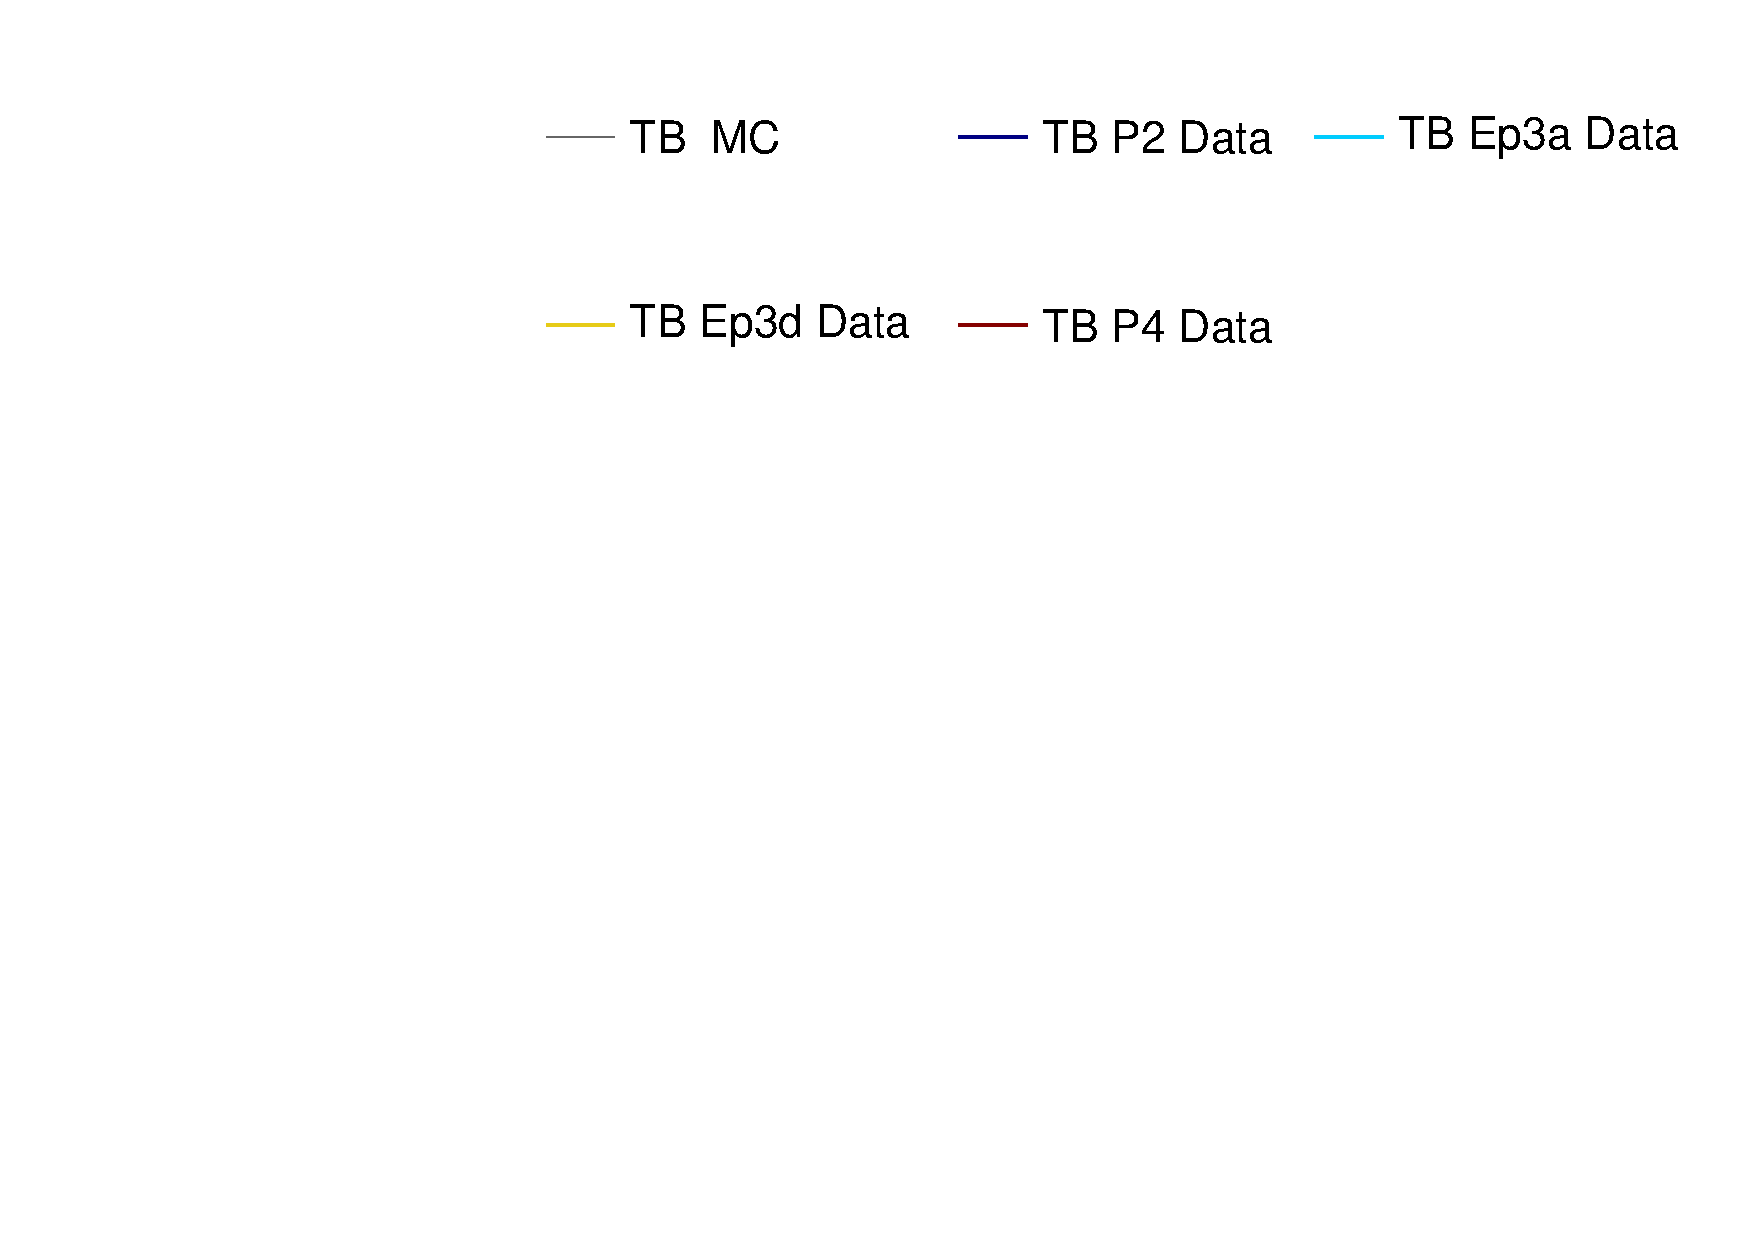
\includegraphics[height=0.2\linewidth]{Plots/Calibana/legend.pdf}
  \end{subfigure}
  \vspace*{2mm}
  
  \begin{subfigure}{0.495\textwidth}
    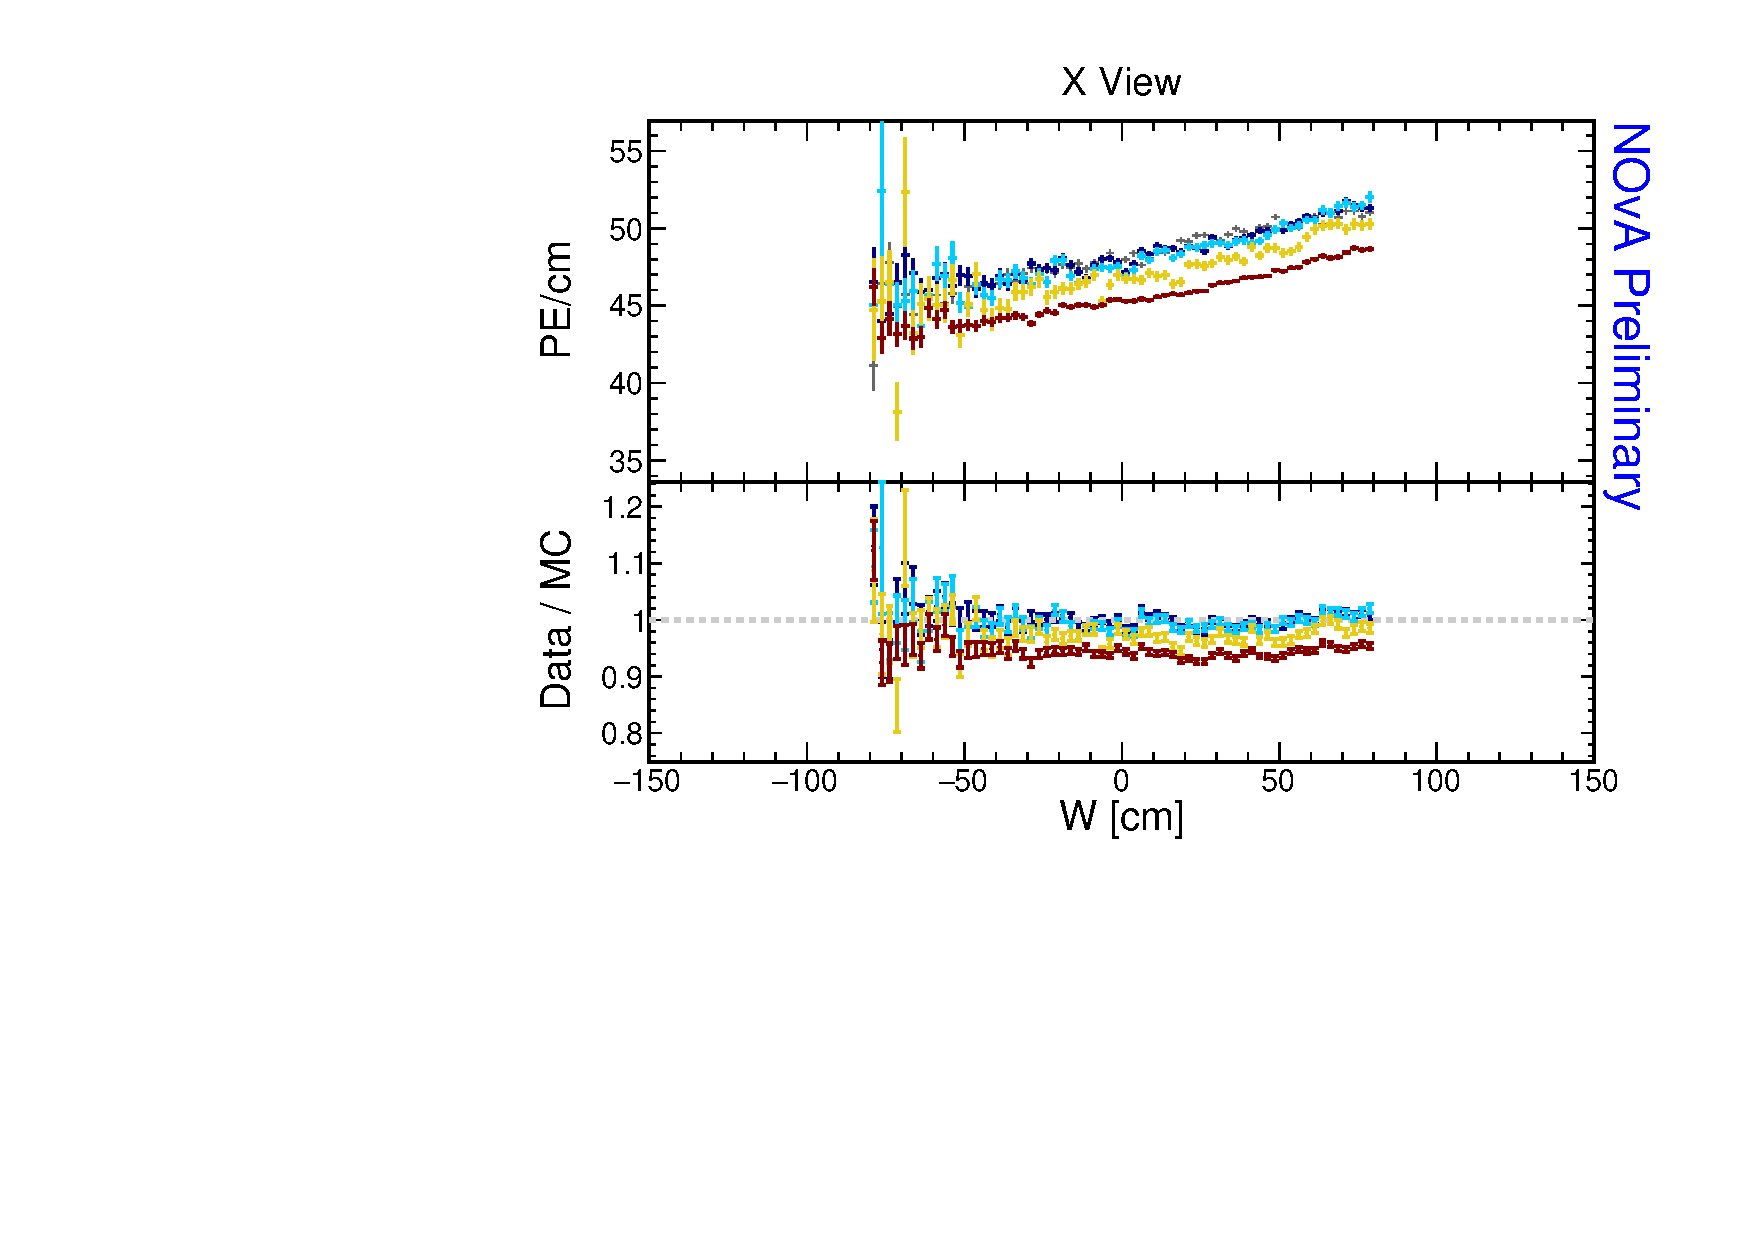
\includegraphics[width=\linewidth]{Plots/Calibana/pecm_w_x.pdf}
  \end{subfigure}
  \begin{subfigure}{0.495\textwidth}
    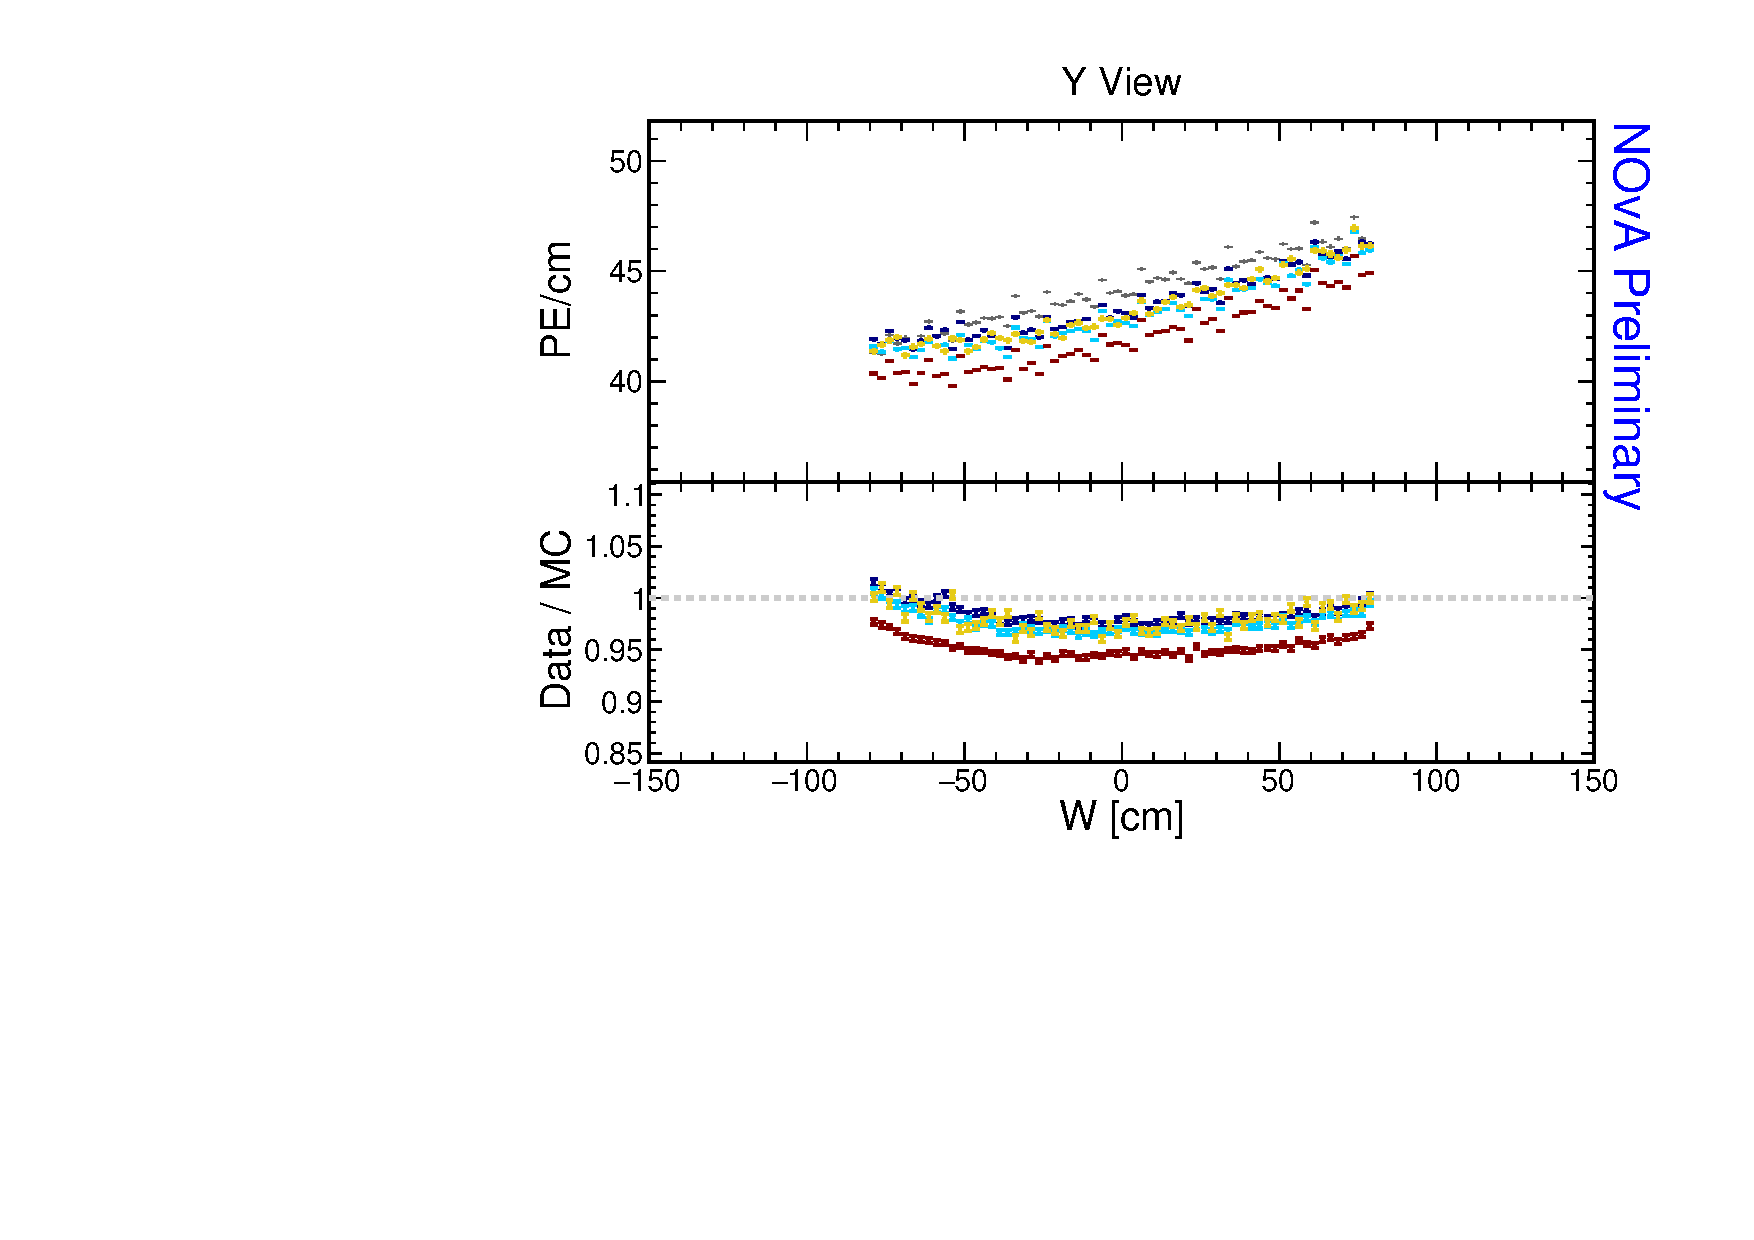
\includegraphics[width=\linewidth]{Plots/Calibana/pecm_w_y.pdf}
  \end{subfigure}
  \begin{subfigure}{0.495\textwidth}
    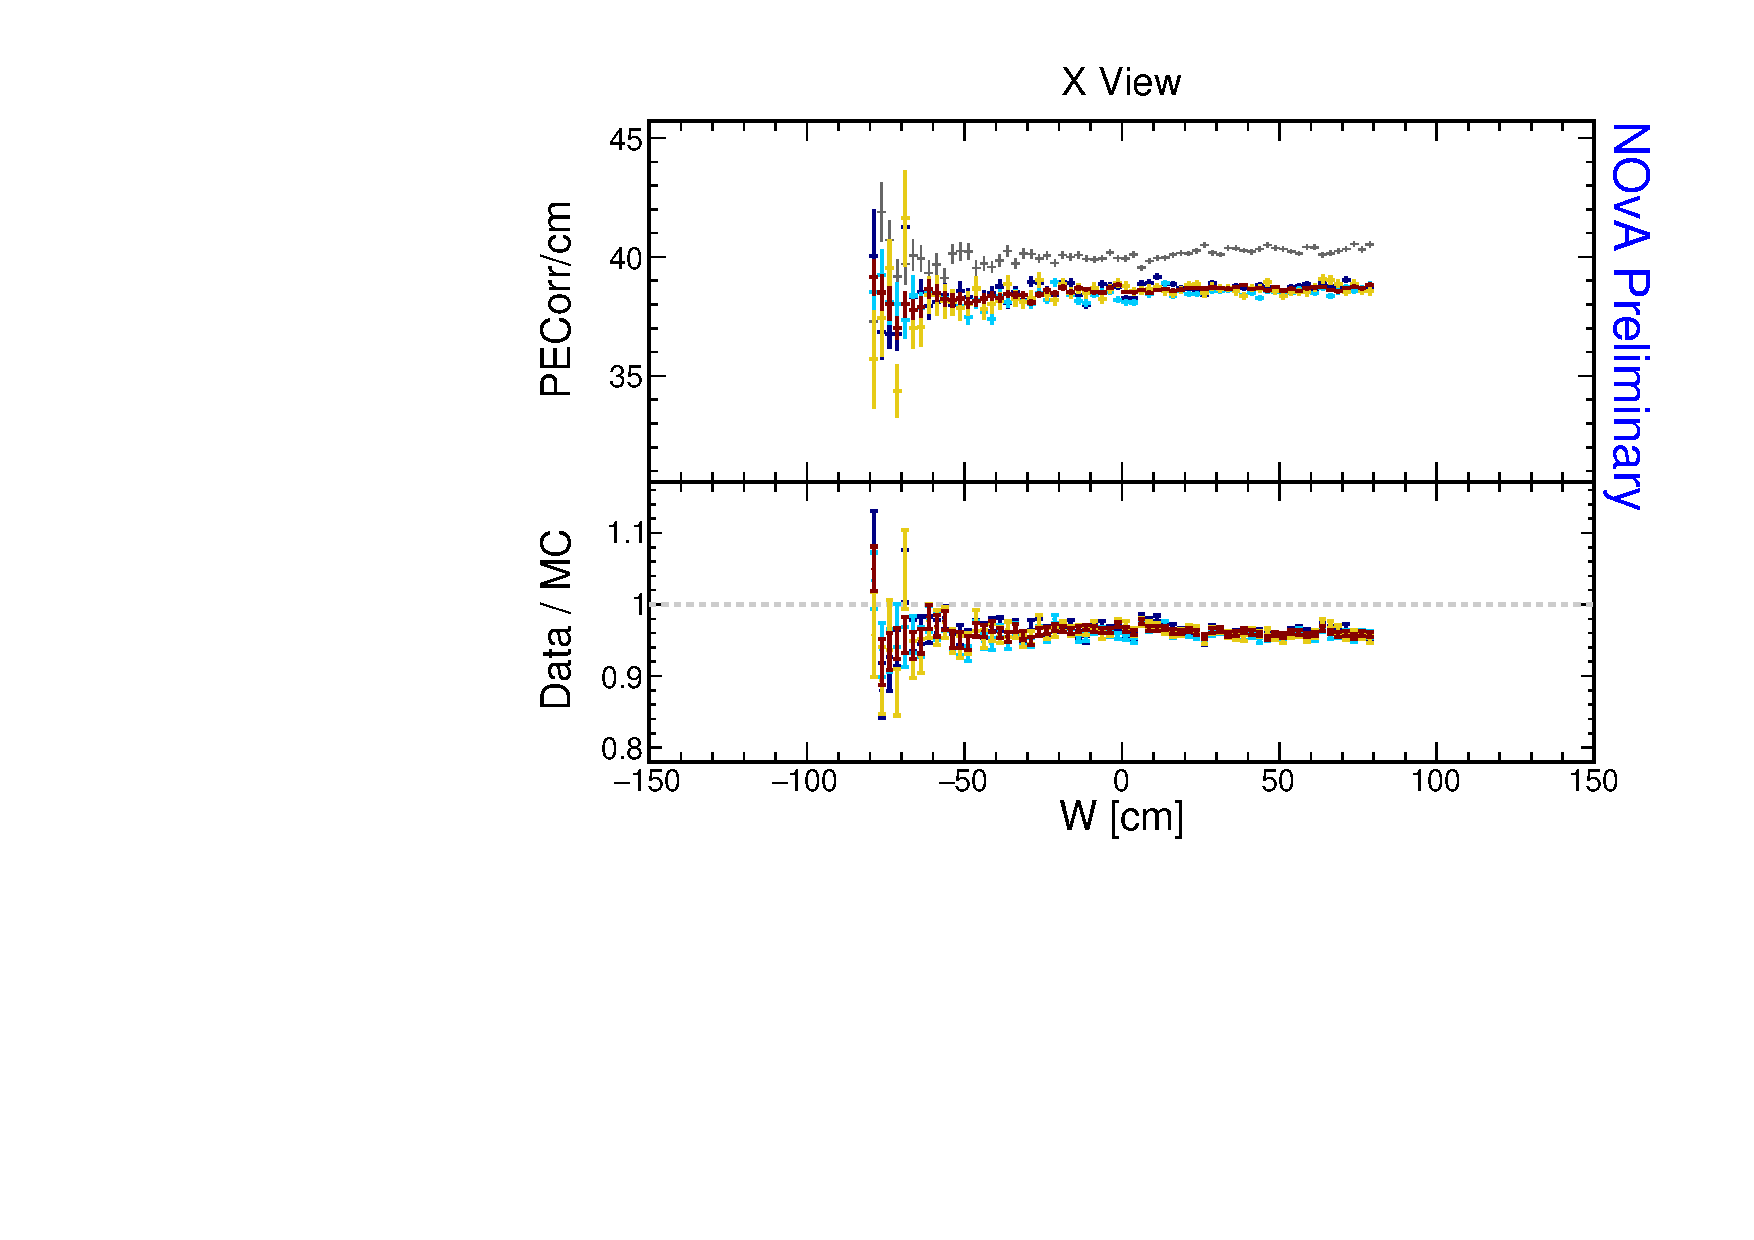
\includegraphics[width=\linewidth]{Plots/Calibana/pecorrcm_w_x.pdf}
  \end{subfigure}
  \begin{subfigure}{0.495\textwidth}
    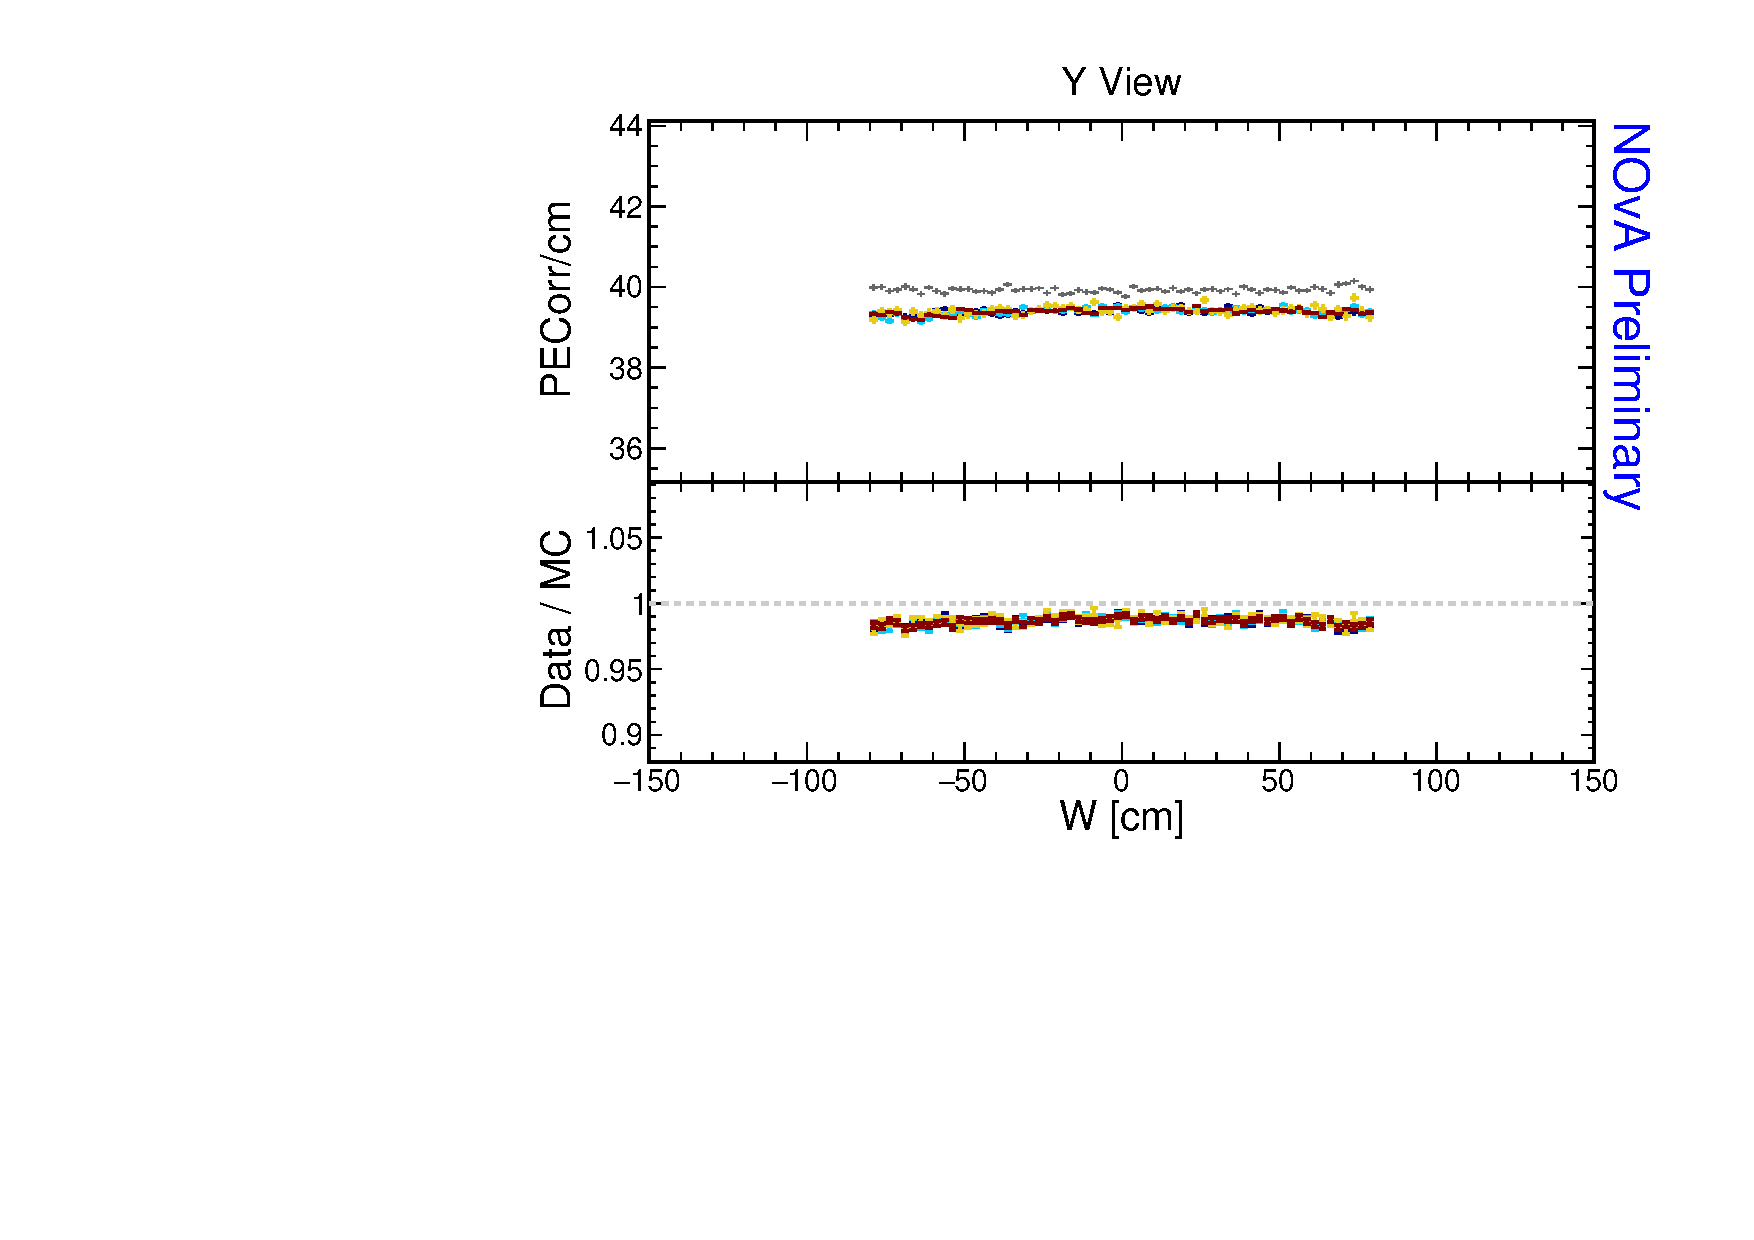
\includegraphics[width=\linewidth]{Plots/Calibana/pecorrcm_w_y.pdf}
  \end{subfigure}
    \begin{subfigure}{0.495\textwidth}
    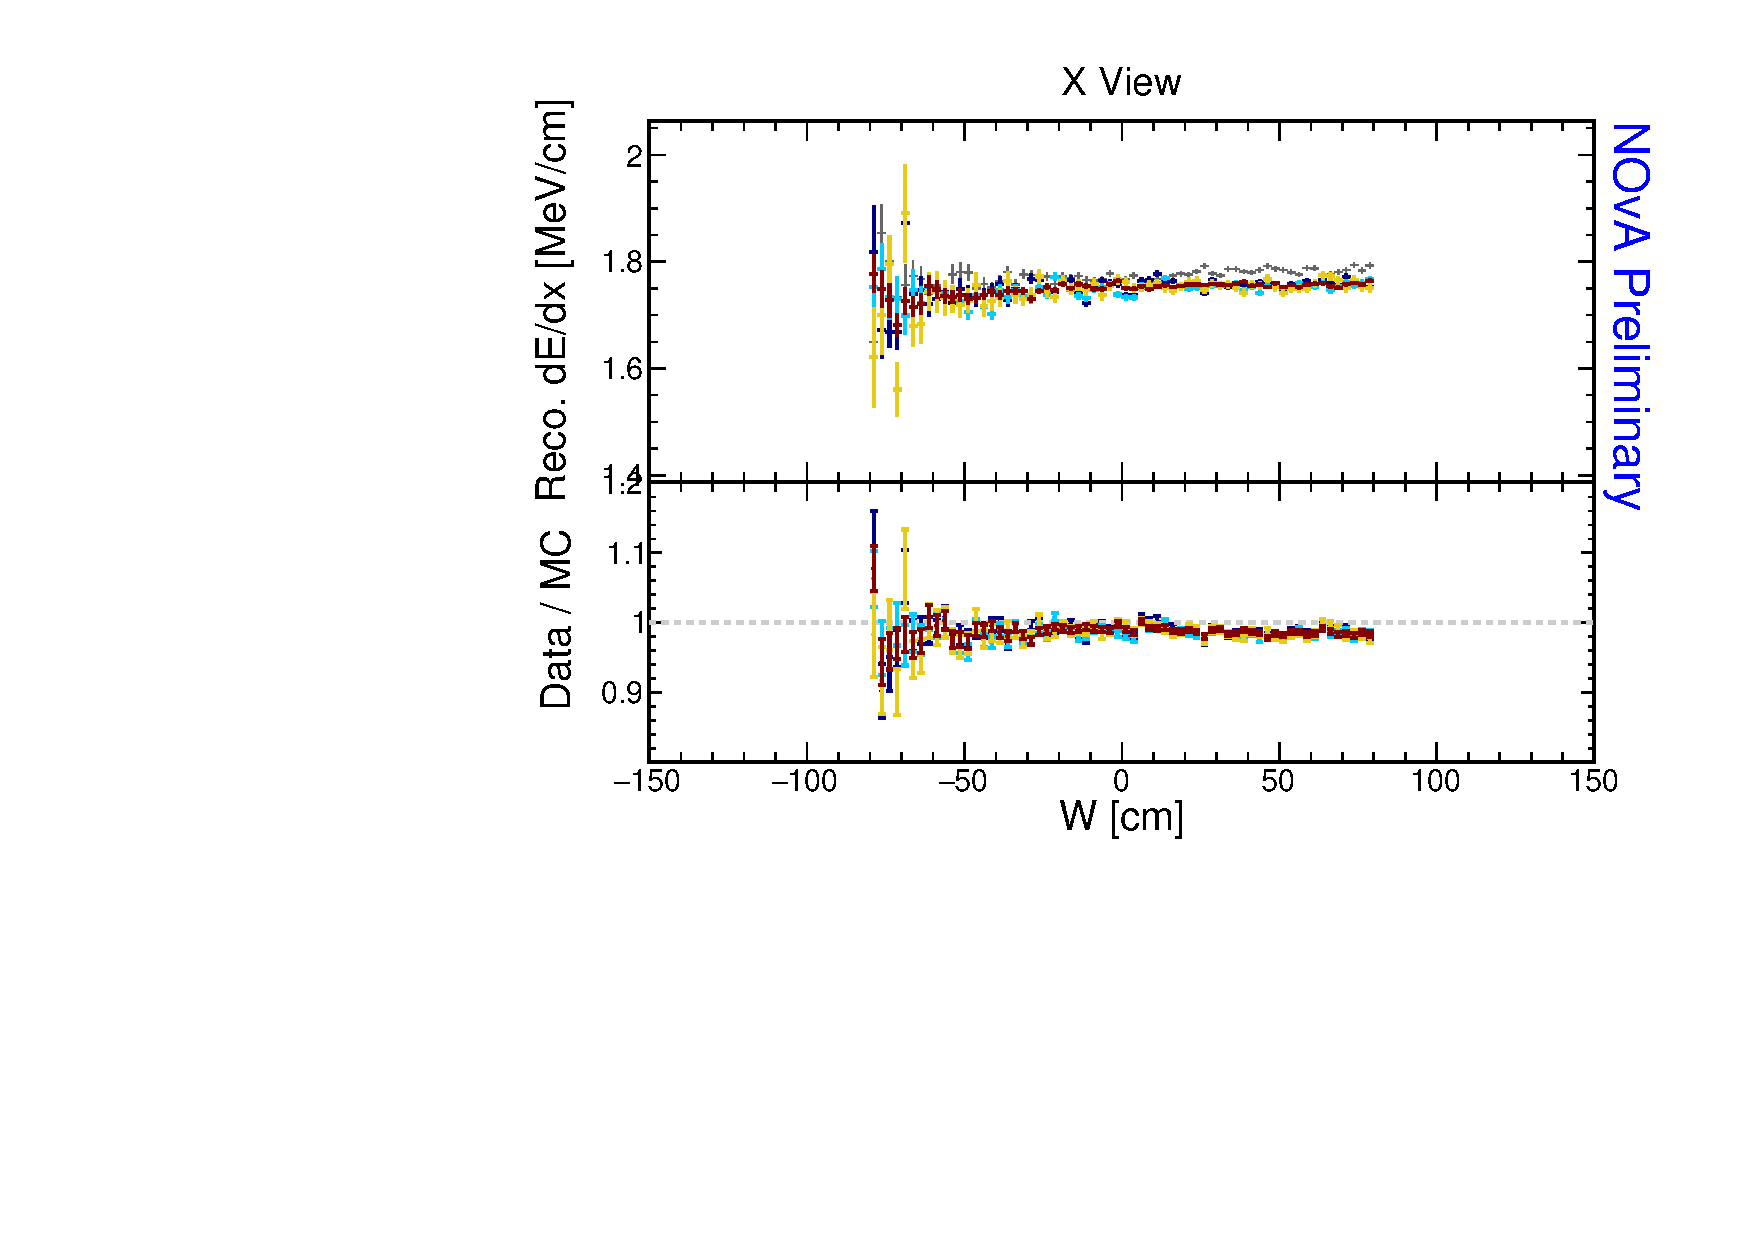
\includegraphics[width=\linewidth]{Plots/Calibana/recomevcm_w_x.pdf}
  \end{subfigure}
  \begin{subfigure}{0.495\textwidth}
    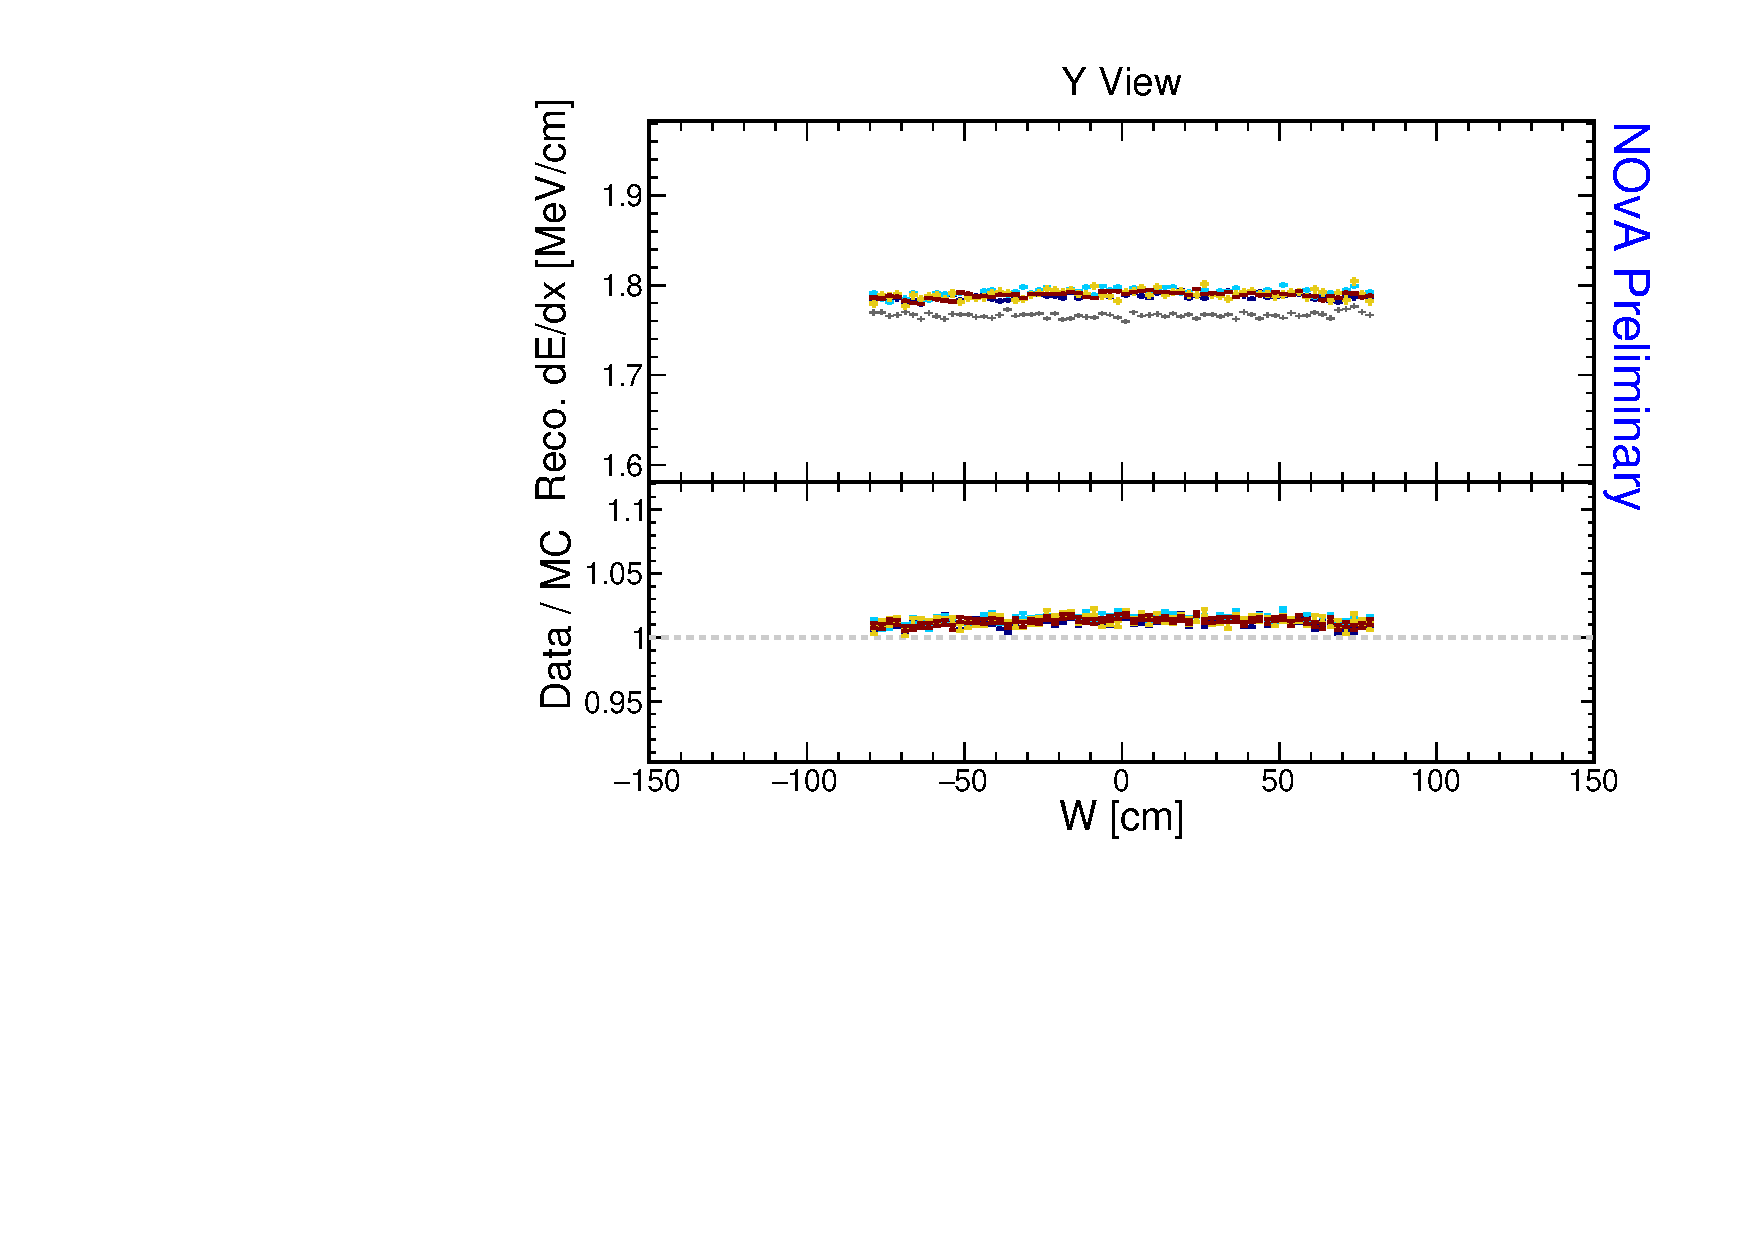
\includegraphics[width=\linewidth]{Plots/Calibana/recomevcm_w_y.pdf}
  \end{subfigure}
  \caption[Energy deposition of stopping muons along cells]{Distributions of stopping muons within a 1-2 m track window from the end of their tracks across the position within a cell for simulation (gray) and all the Test Beam data samples. The top row shows the energy deposition before any correction, middle row after relative calibration corrections and bottom row after full calibration corrections. The left column shows the X view (vertical planes) and right column the Y view (horizontal planes).}
  %\label{fig:AbsCalibW1}
\end{figure}

\begin{figure}[!ht]
  \begin{subfigure}{\textwidth}
  \centering
    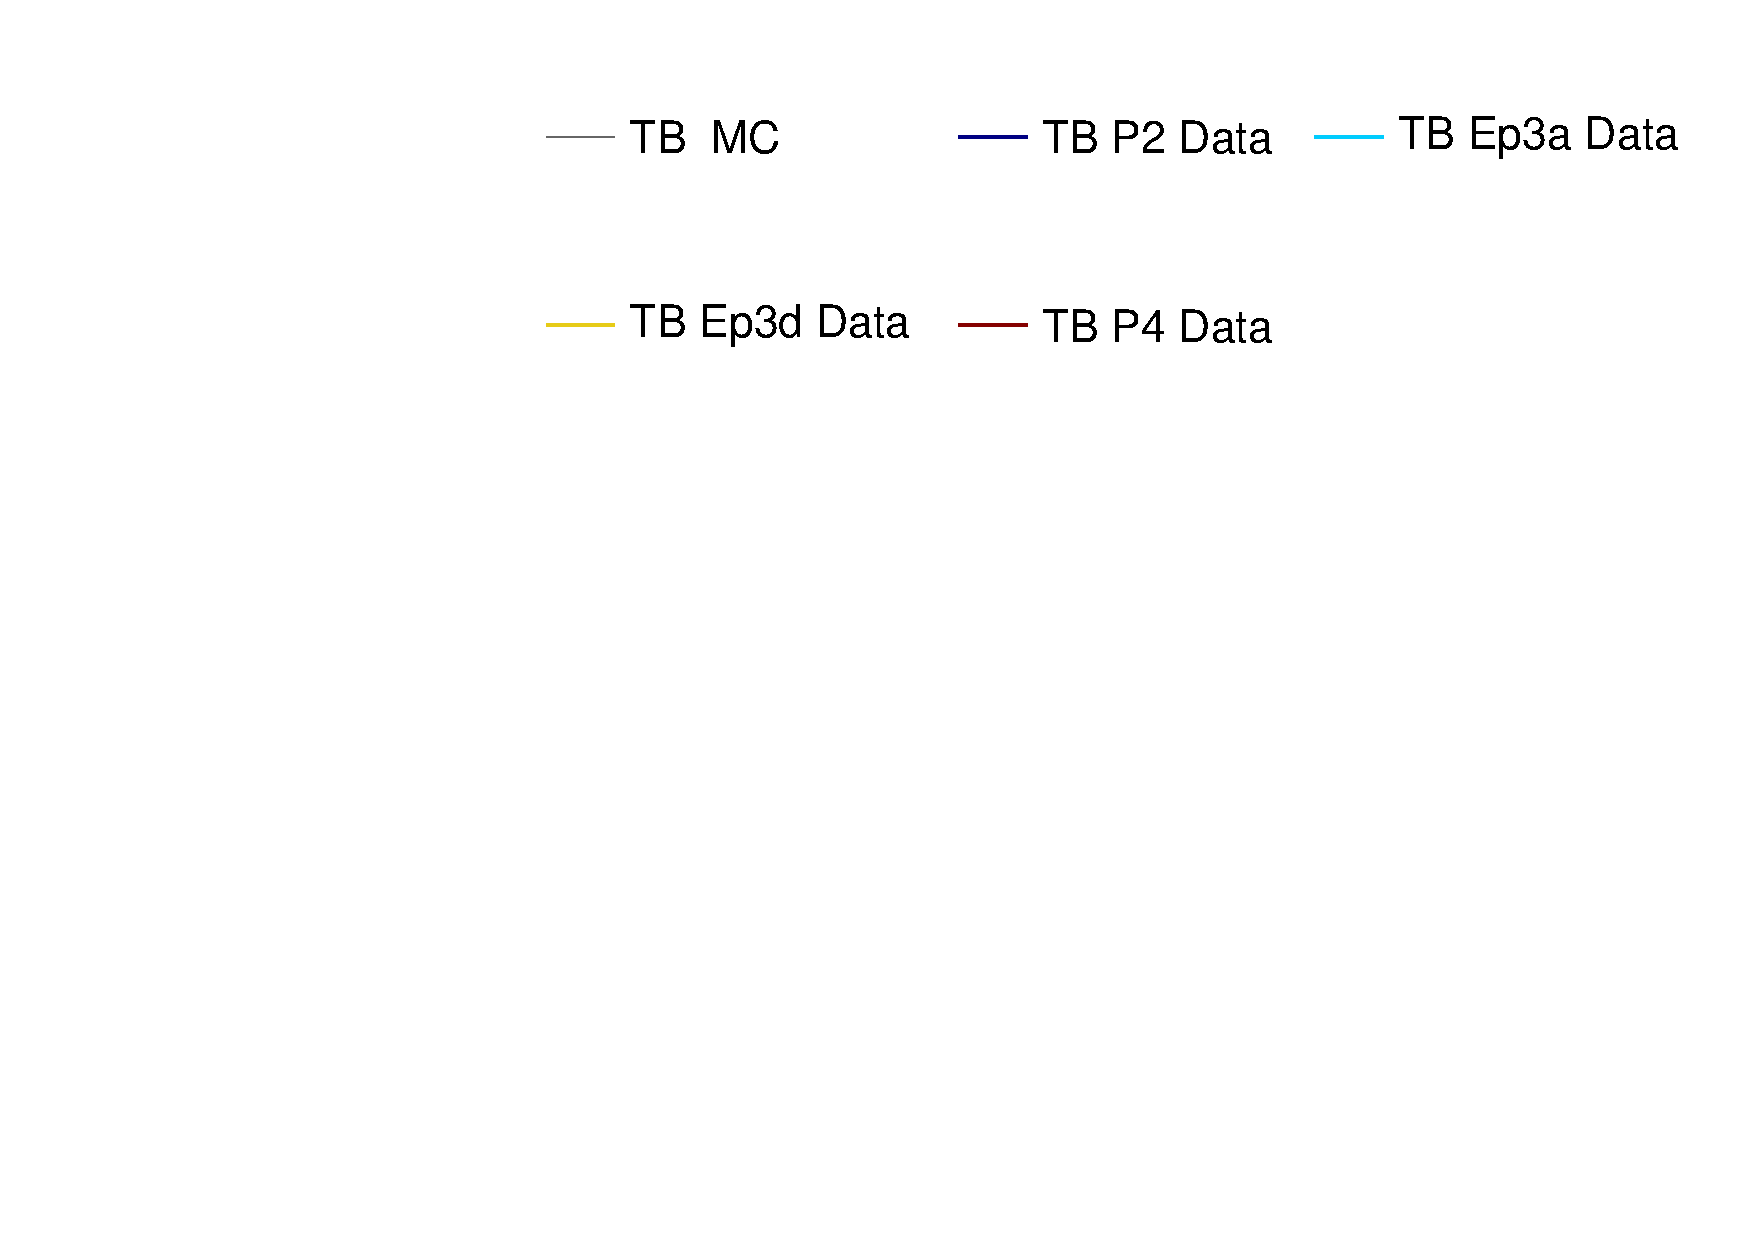
\includegraphics[height=0.2\linewidth]{Plots/Calibana/legend.pdf}
  \end{subfigure}
  \vspace*{2mm}

  \begin{subfigure}{0.495\textwidth}
    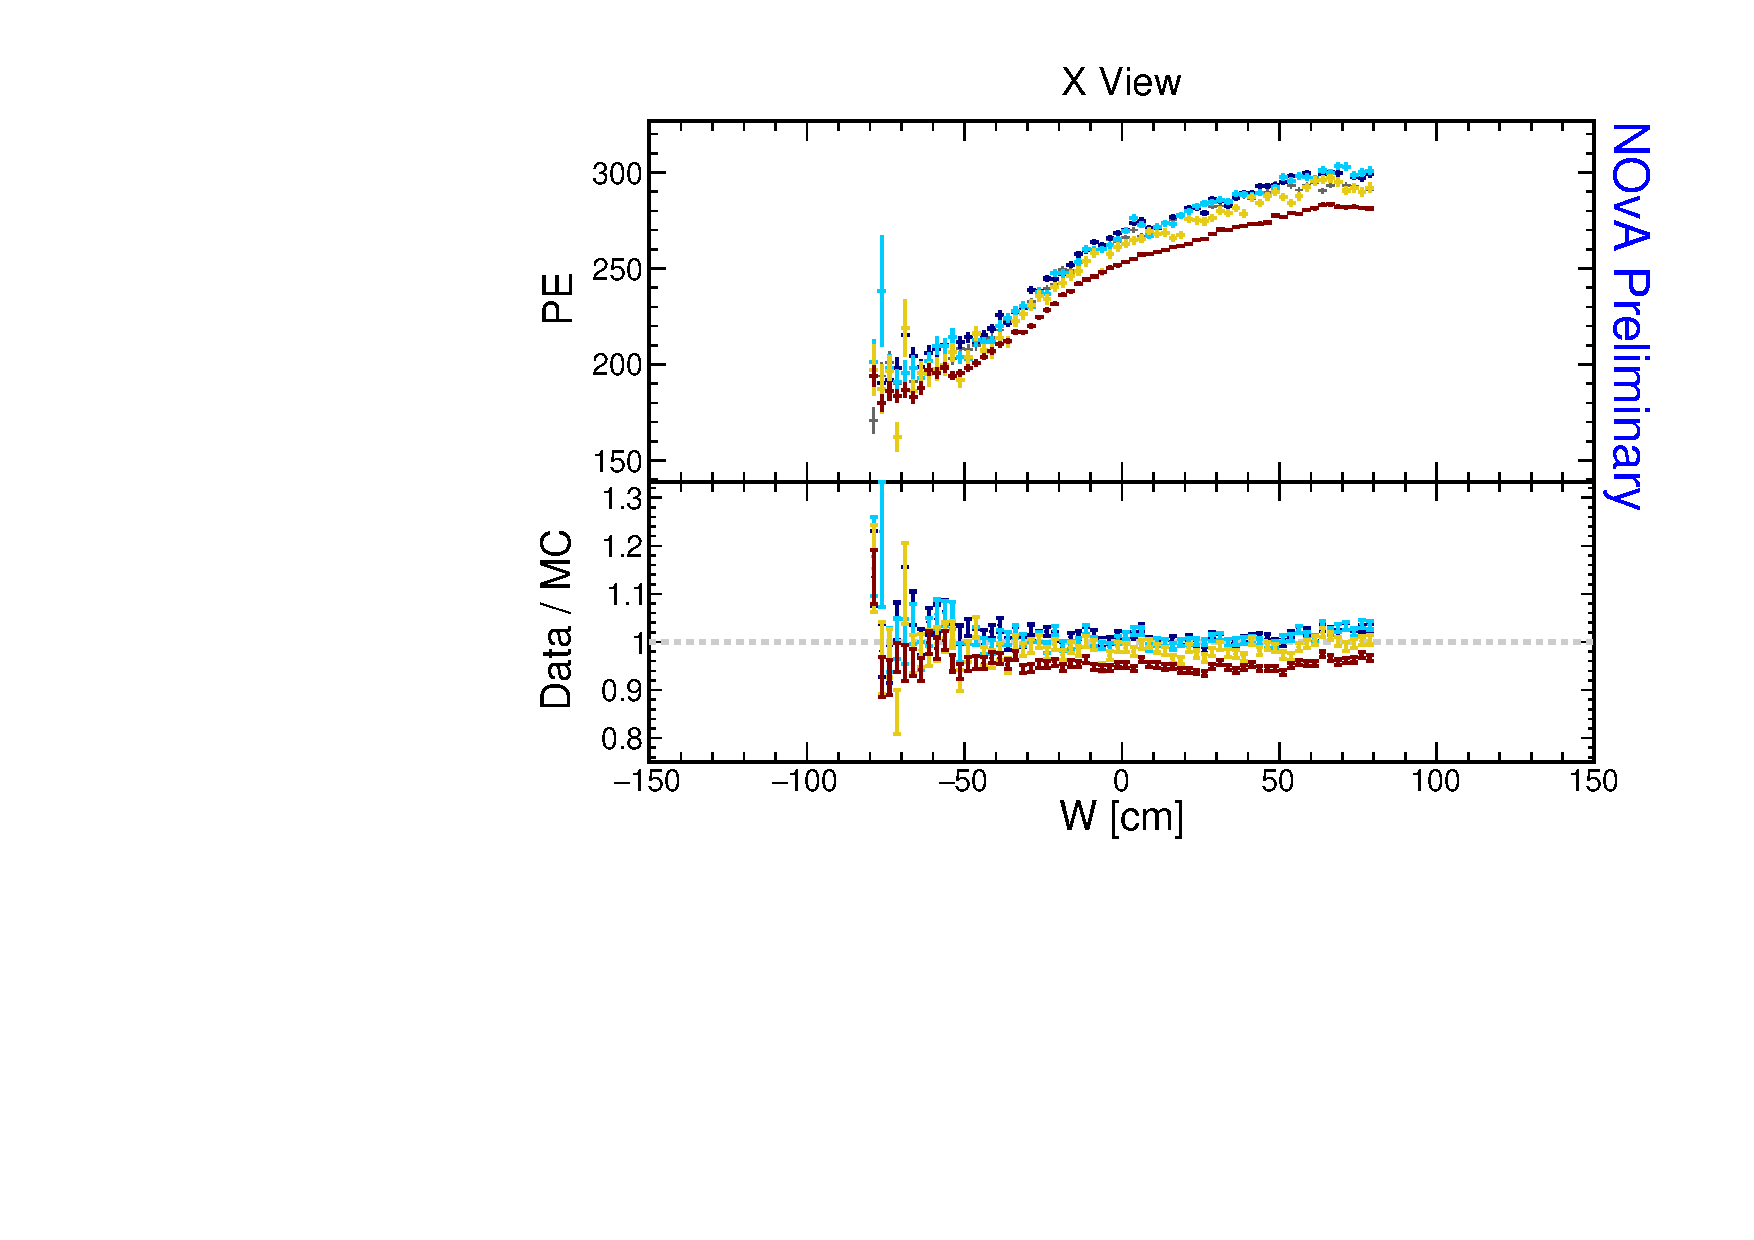
\includegraphics[width=\linewidth]{Plots/Calibana/pe_w_x.pdf}
  \end{subfigure}
  \begin{subfigure}{0.495\textwidth}
    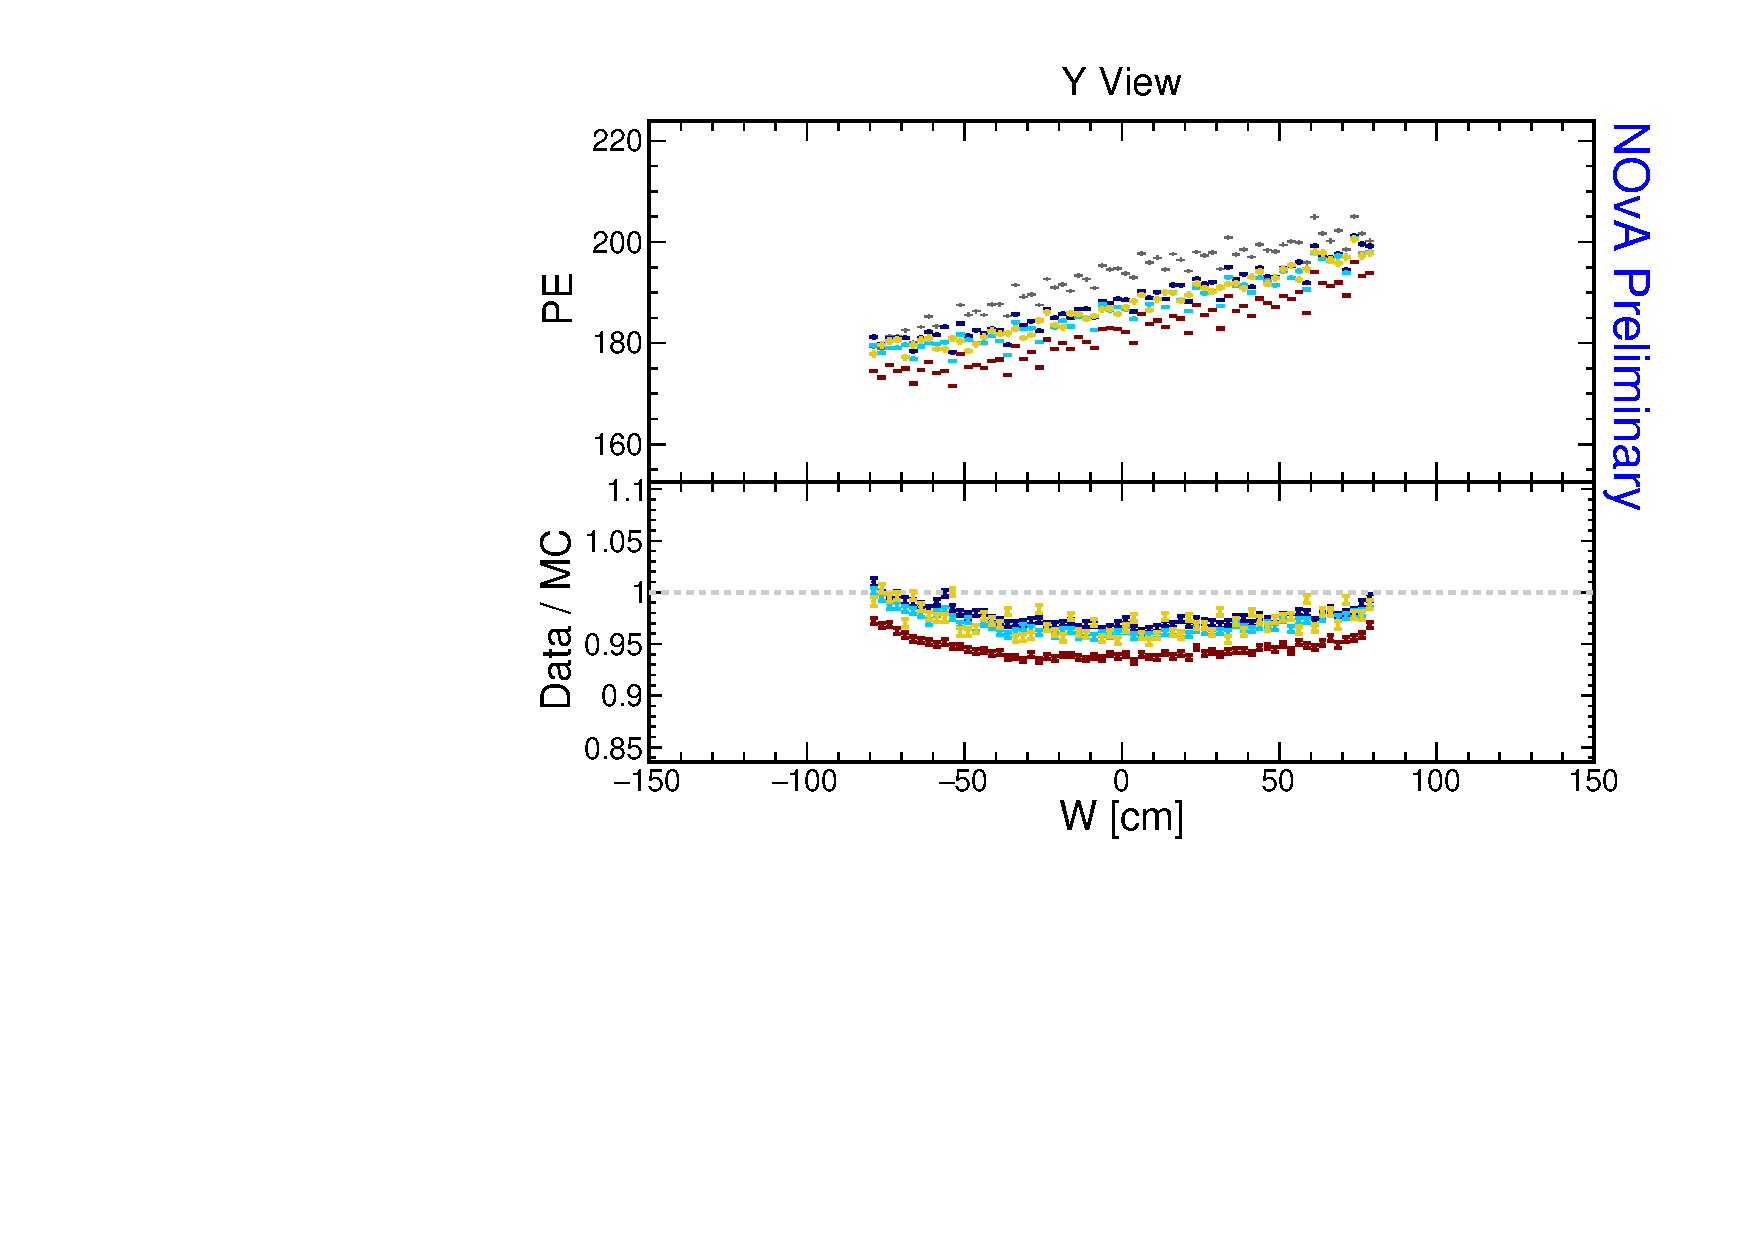
\includegraphics[width=\linewidth]{Plots/Calibana/pe_w_y.pdf}
  \end{subfigure}
  \begin{subfigure}{0.495\textwidth}
    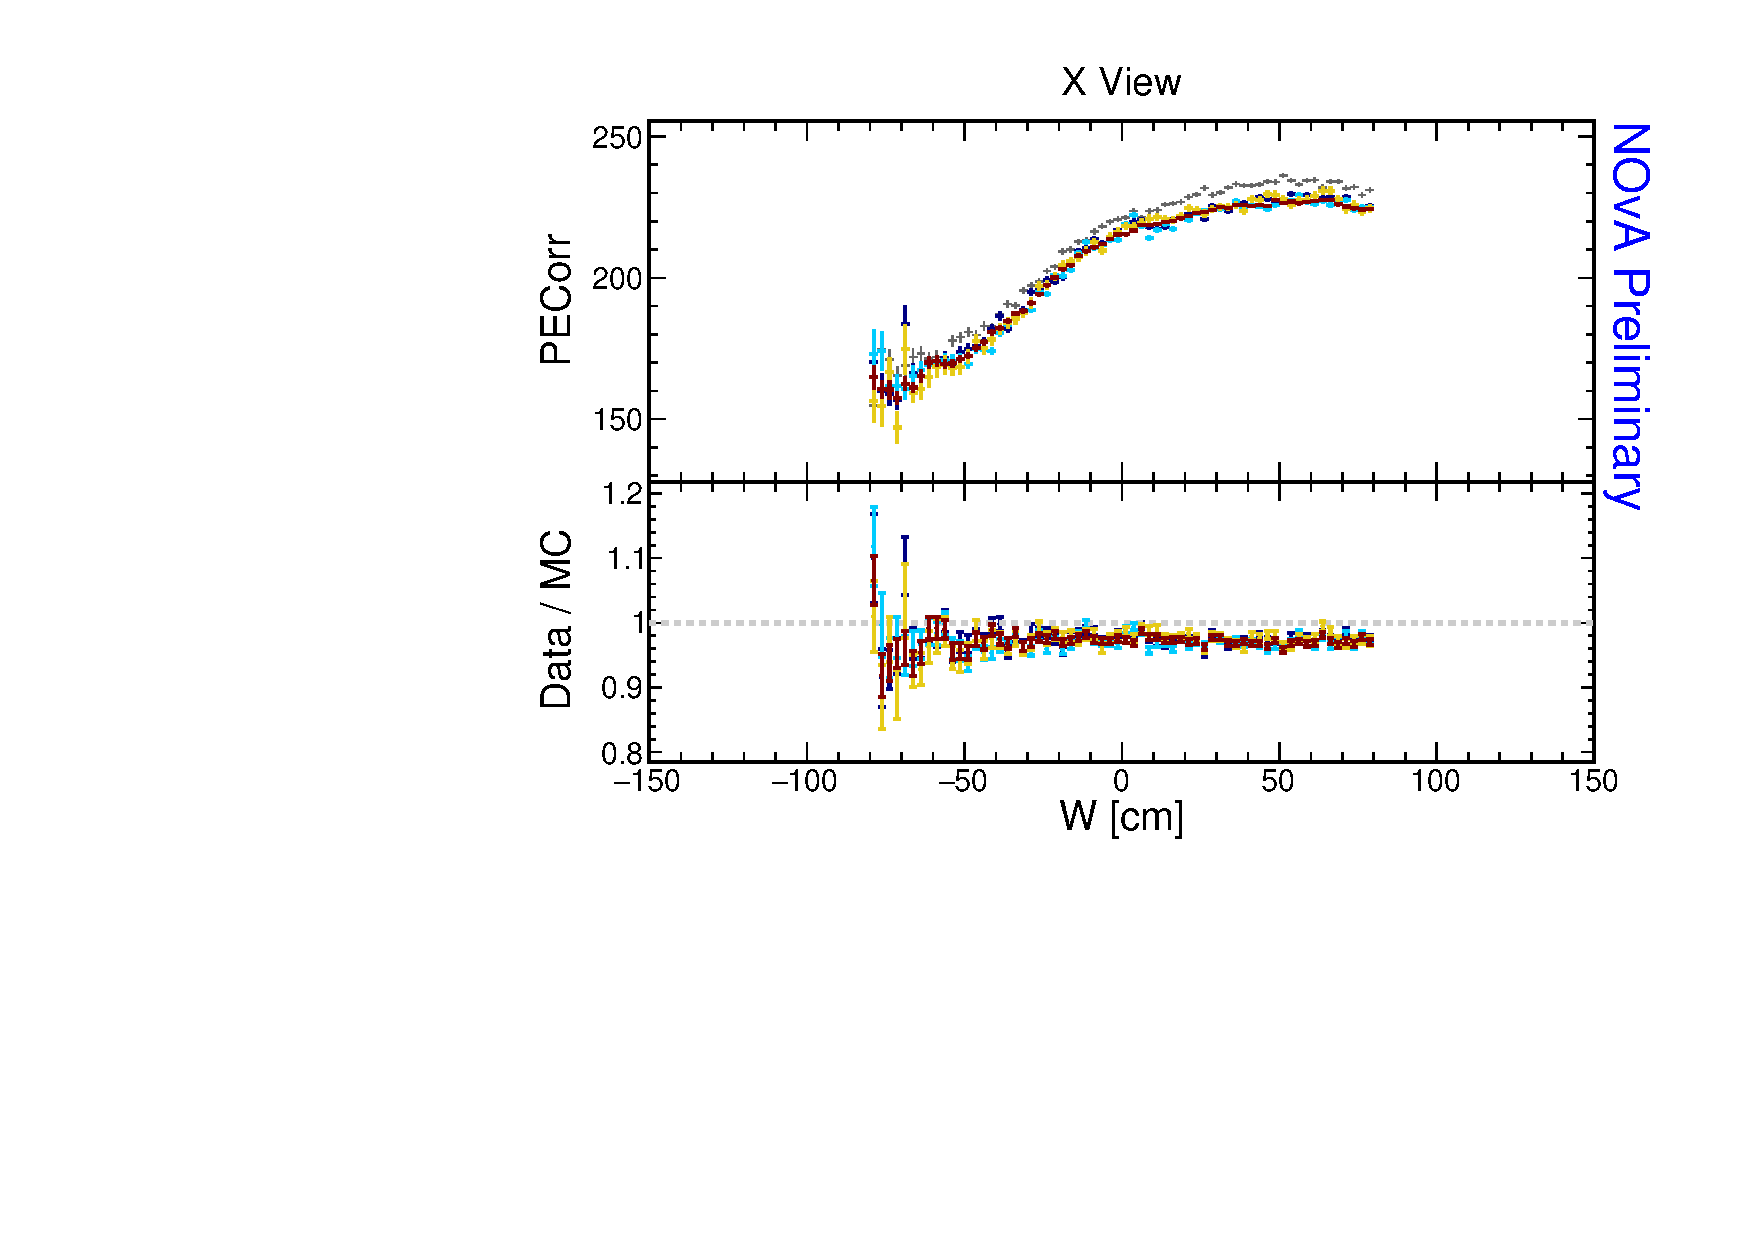
\includegraphics[width=\linewidth]{Plots/Calibana/pecorr_w_x.pdf}
  \end{subfigure}
  \begin{subfigure}{0.495\textwidth}
    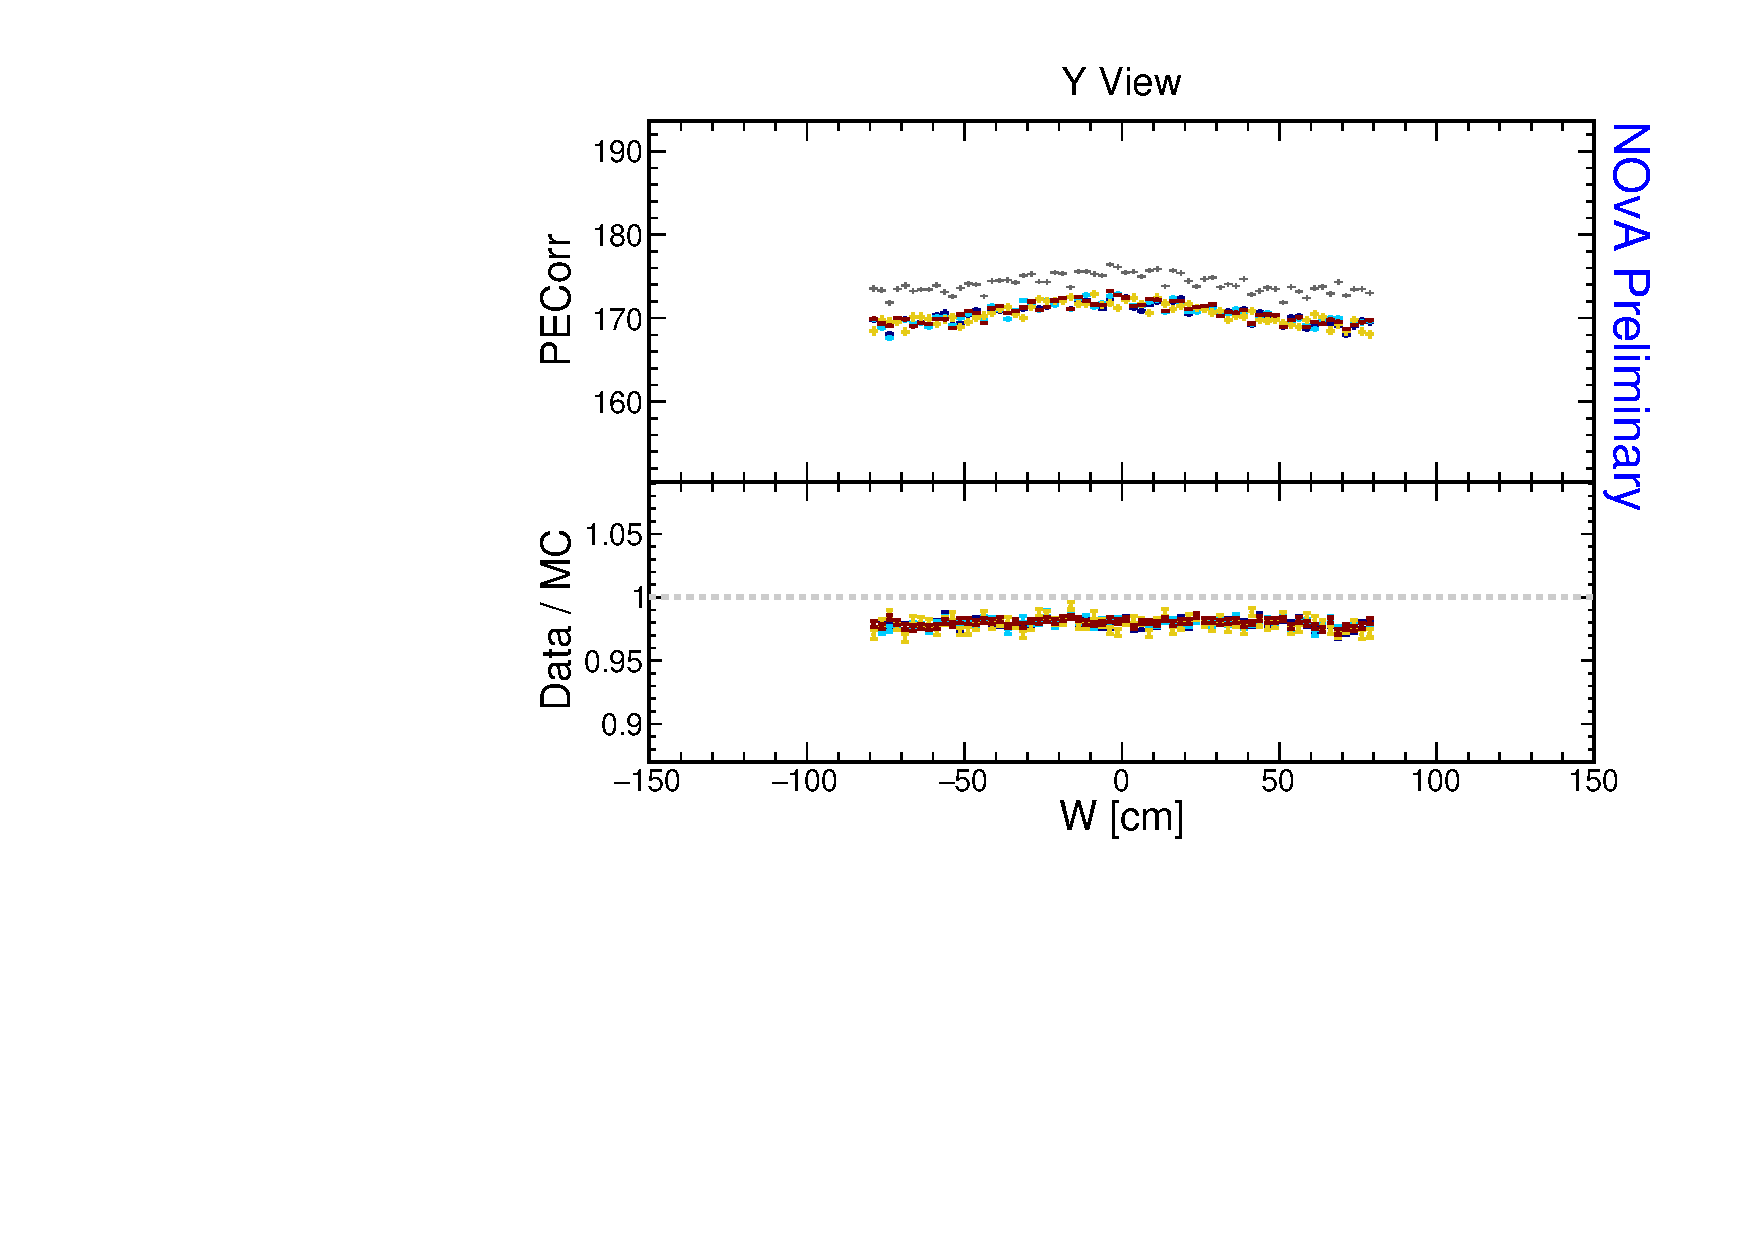
\includegraphics[width=\linewidth]{Plots/Calibana/pecorr_w_y.pdf}
  \end{subfigure}
  \begin{subfigure}{0.495\textwidth}
    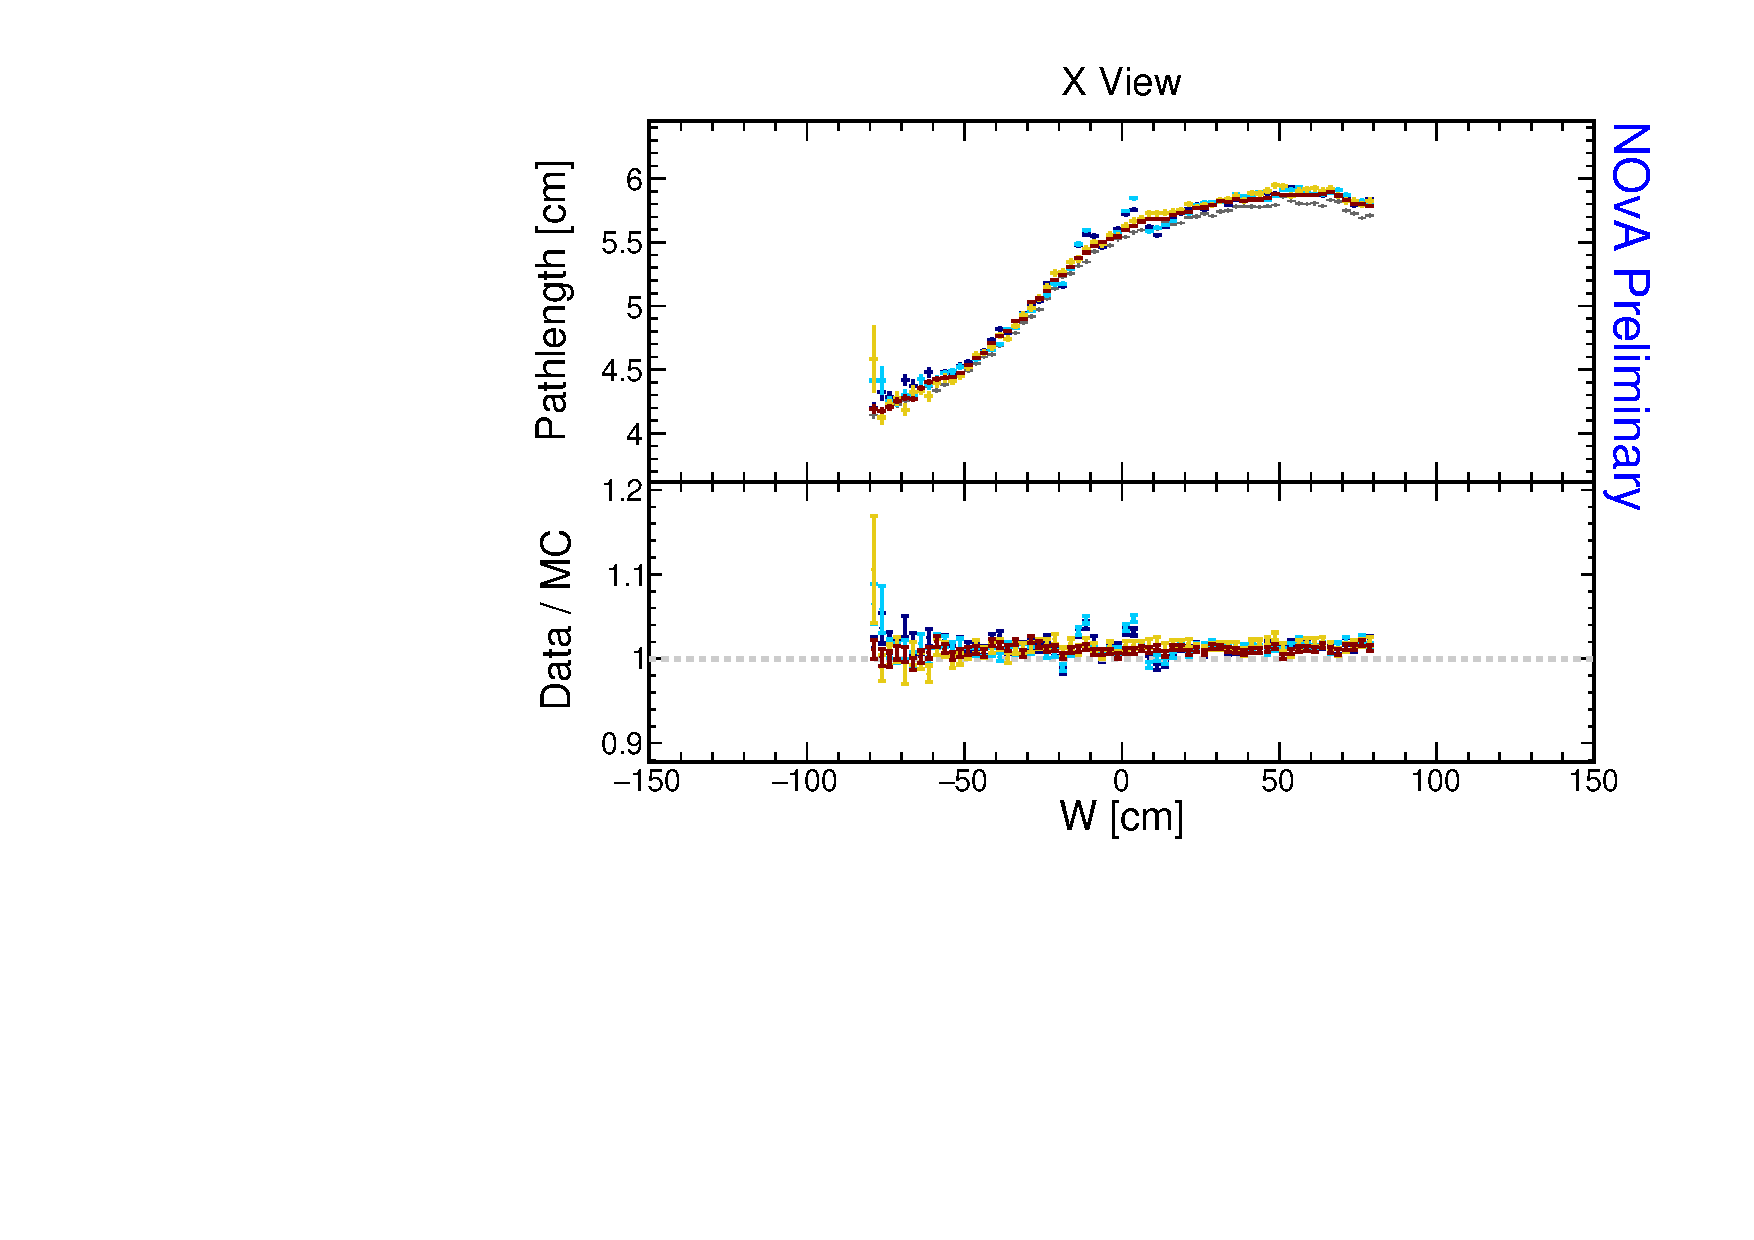
\includegraphics[width=\linewidth]{Plots/Calibana/cm_w_x.pdf}
  \end{subfigure}
  \begin{subfigure}{0.495\textwidth}
    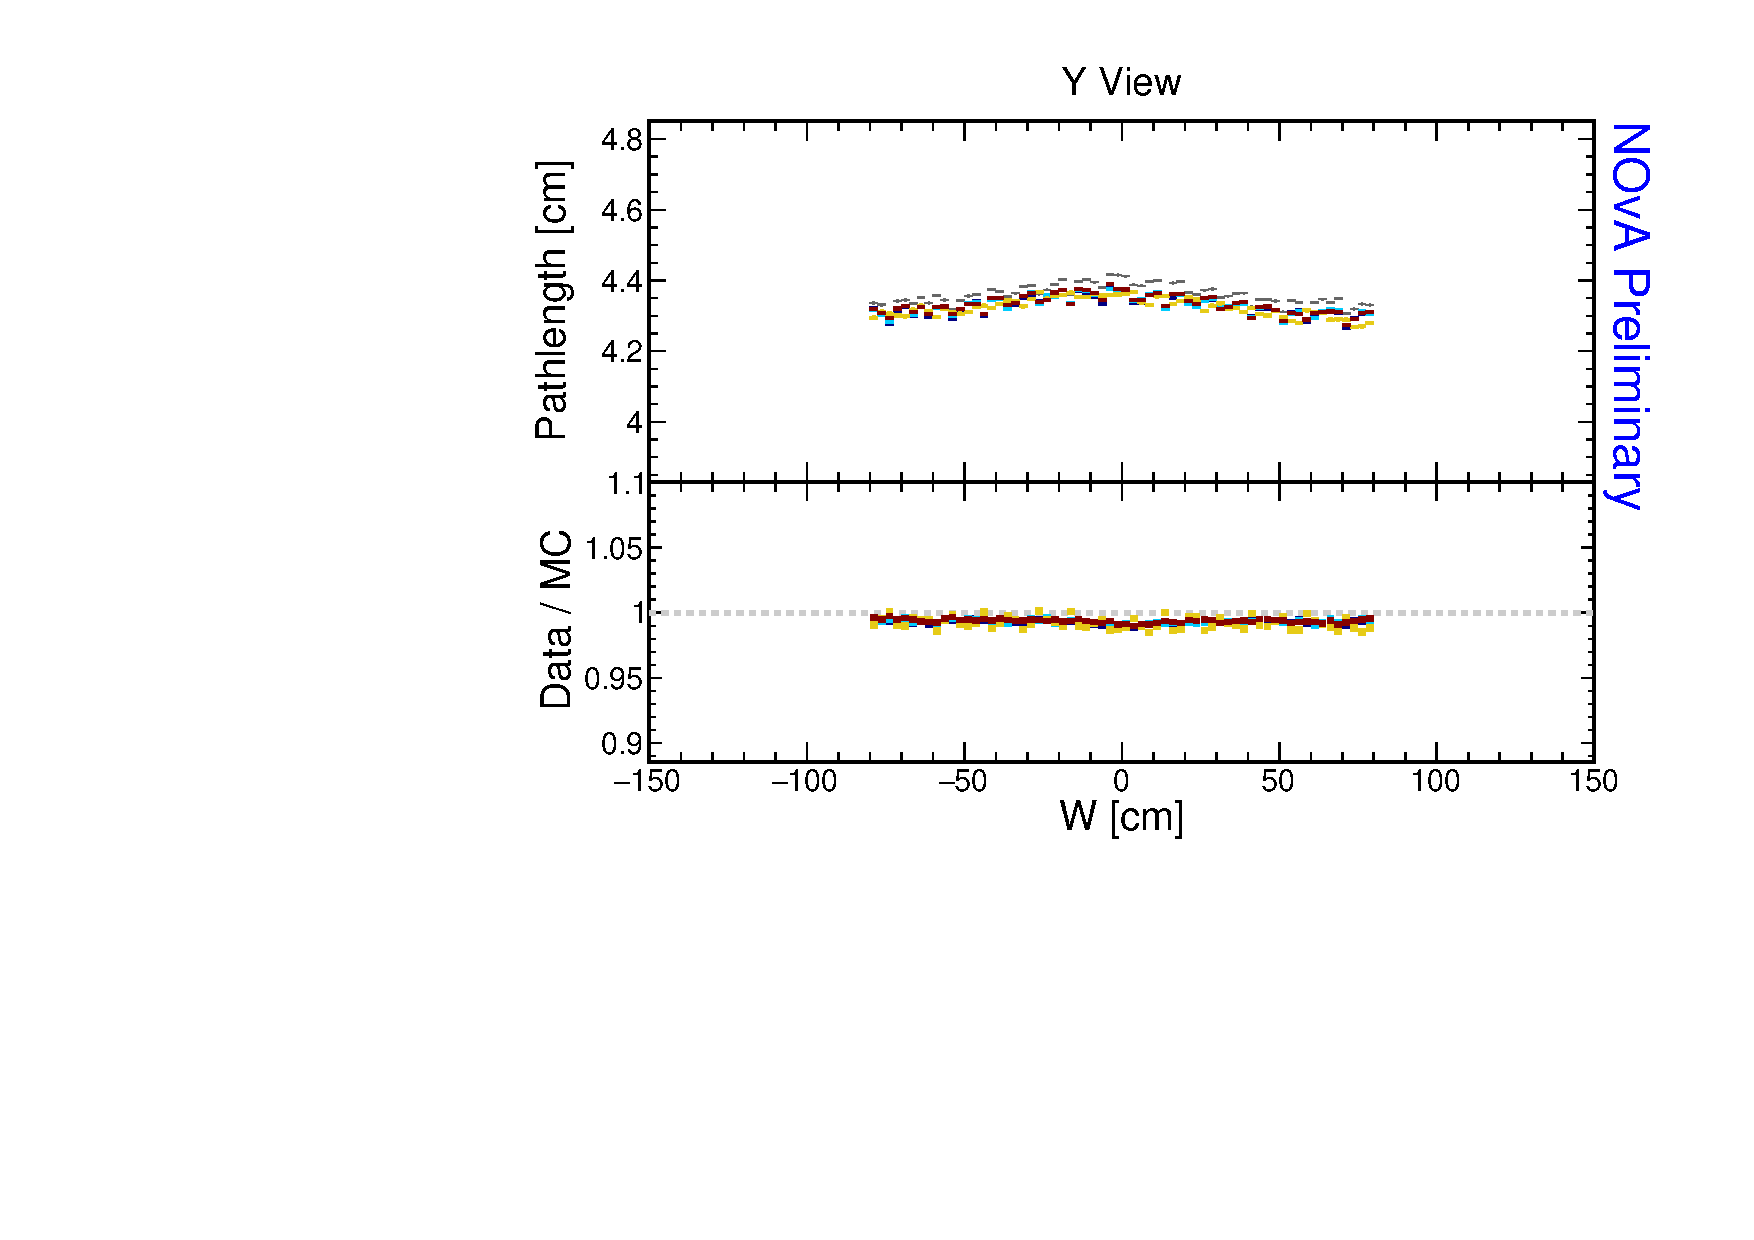
\includegraphics[width=\linewidth]{Plots/Calibana/cm_w_y.pdf}
  \end{subfigure}
  \caption[Calibration variables of stopping muons along cells]{Distributions of stopping muons within a 1-2 m track window from the end of their tracks across the position within a cell for simulation (gray) and all the Test Beam data samples. The top row shows the number of recorded photo electrons before any corrections, middle row shows the same after relative calibration corrections and bottom row shows the path length through the cell. The left column shows the X view (vertical planes) and right column the Y view (horizontal planes).}
  %\label{fig:AbsCalibW2}
\end{figure}

\begin{figure}[!ht]
  \begin{subfigure}{\textwidth}
  \centering
    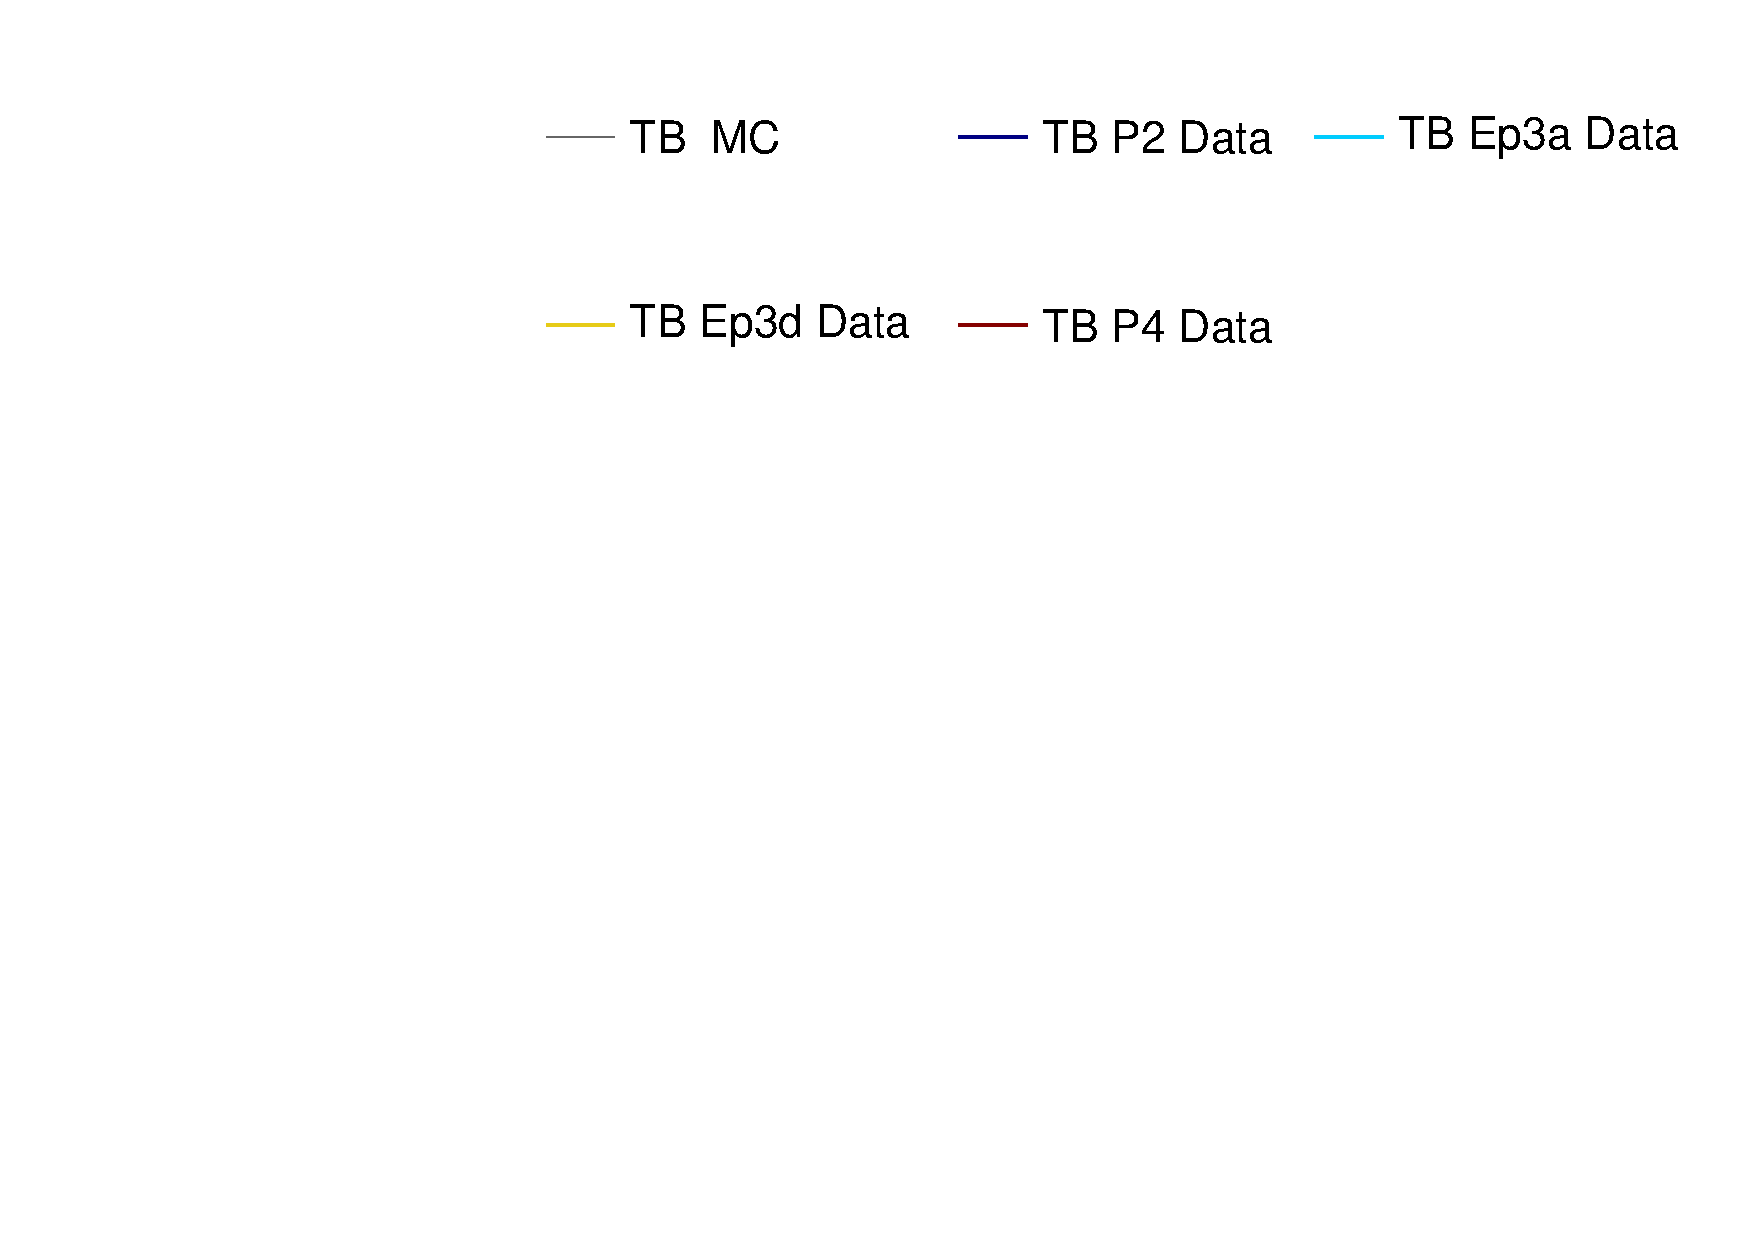
\includegraphics[height=0.2\linewidth]{Plots/Calibana/legend.pdf}
  \end{subfigure}
  \vspace*{2mm}

  \begin{subfigure}{0.495\textwidth}
    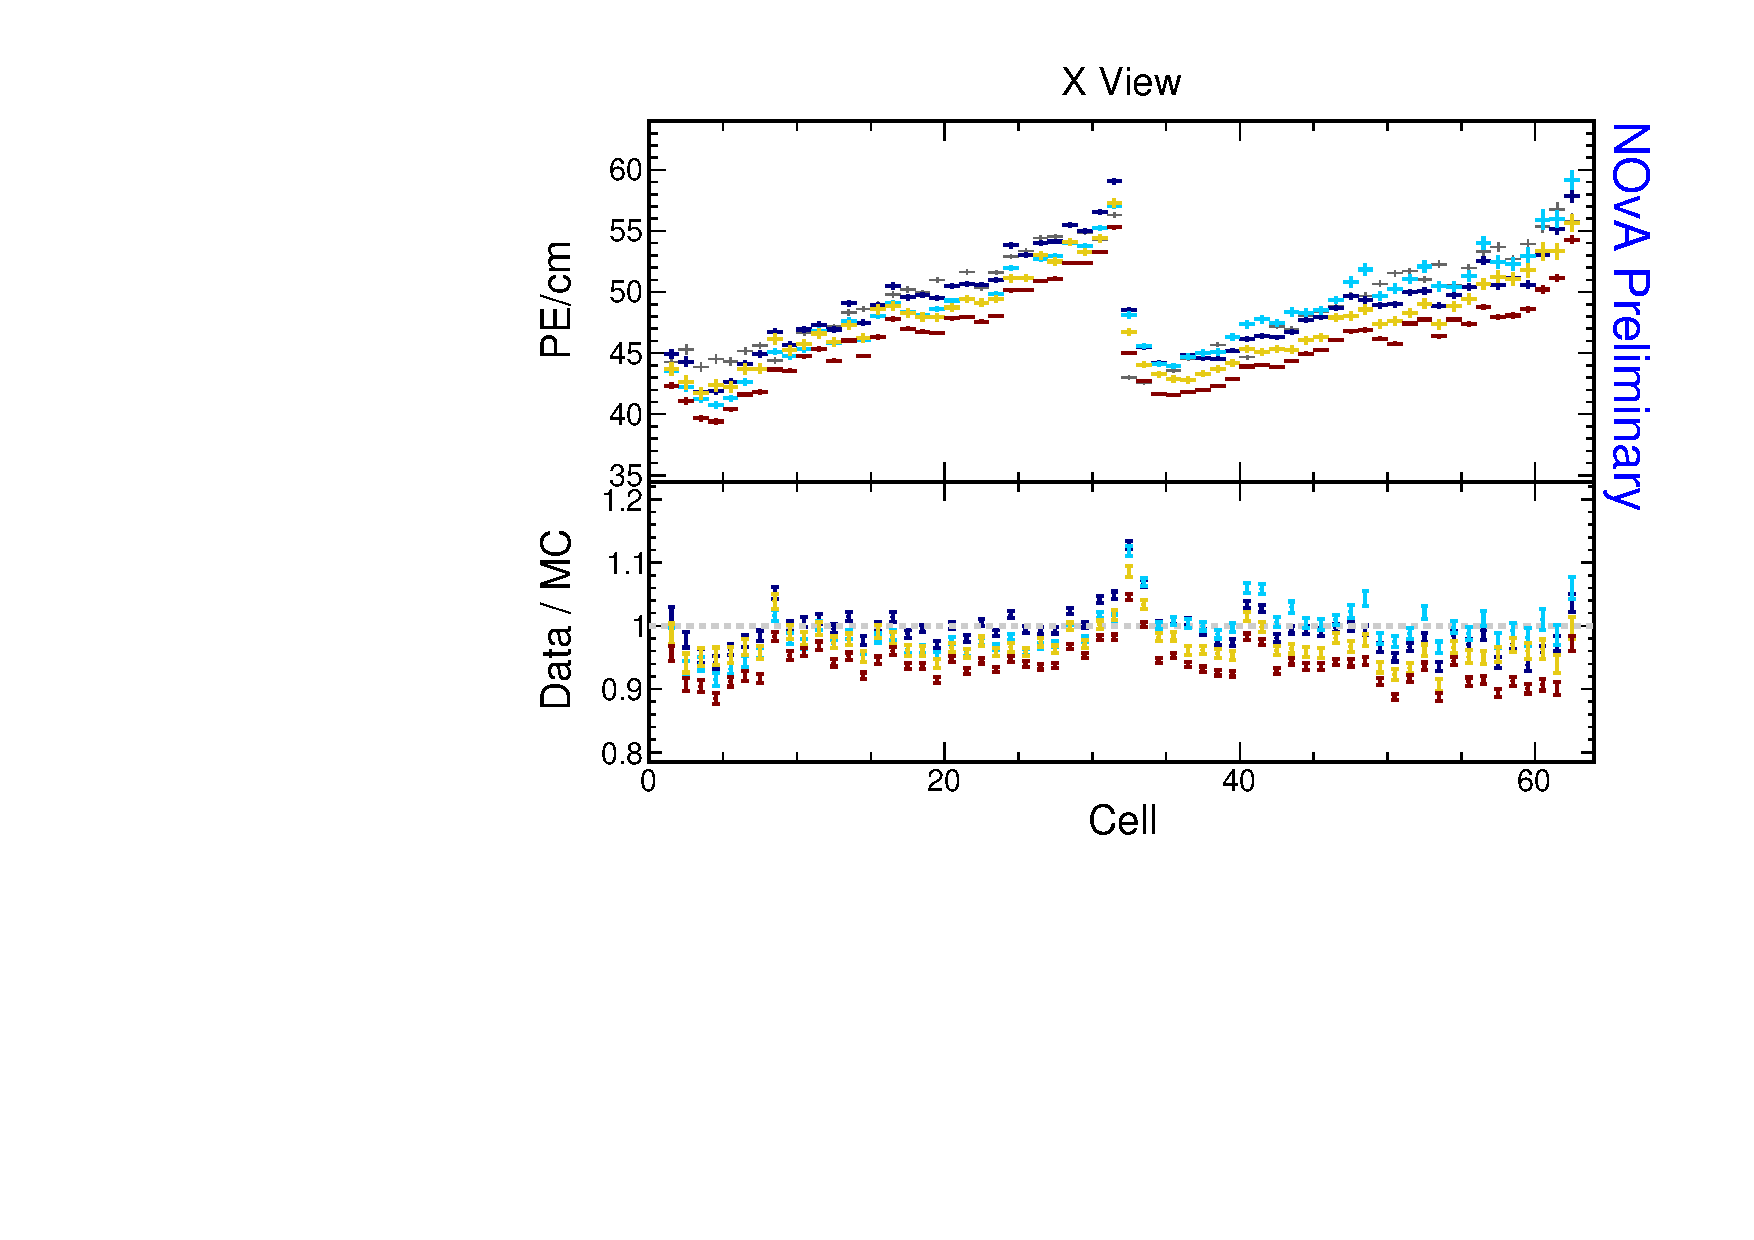
\includegraphics[width=\linewidth]{Plots/Calibana/pecm_cell_x.pdf}
  \end{subfigure}
  \begin{subfigure}{0.495\textwidth}
    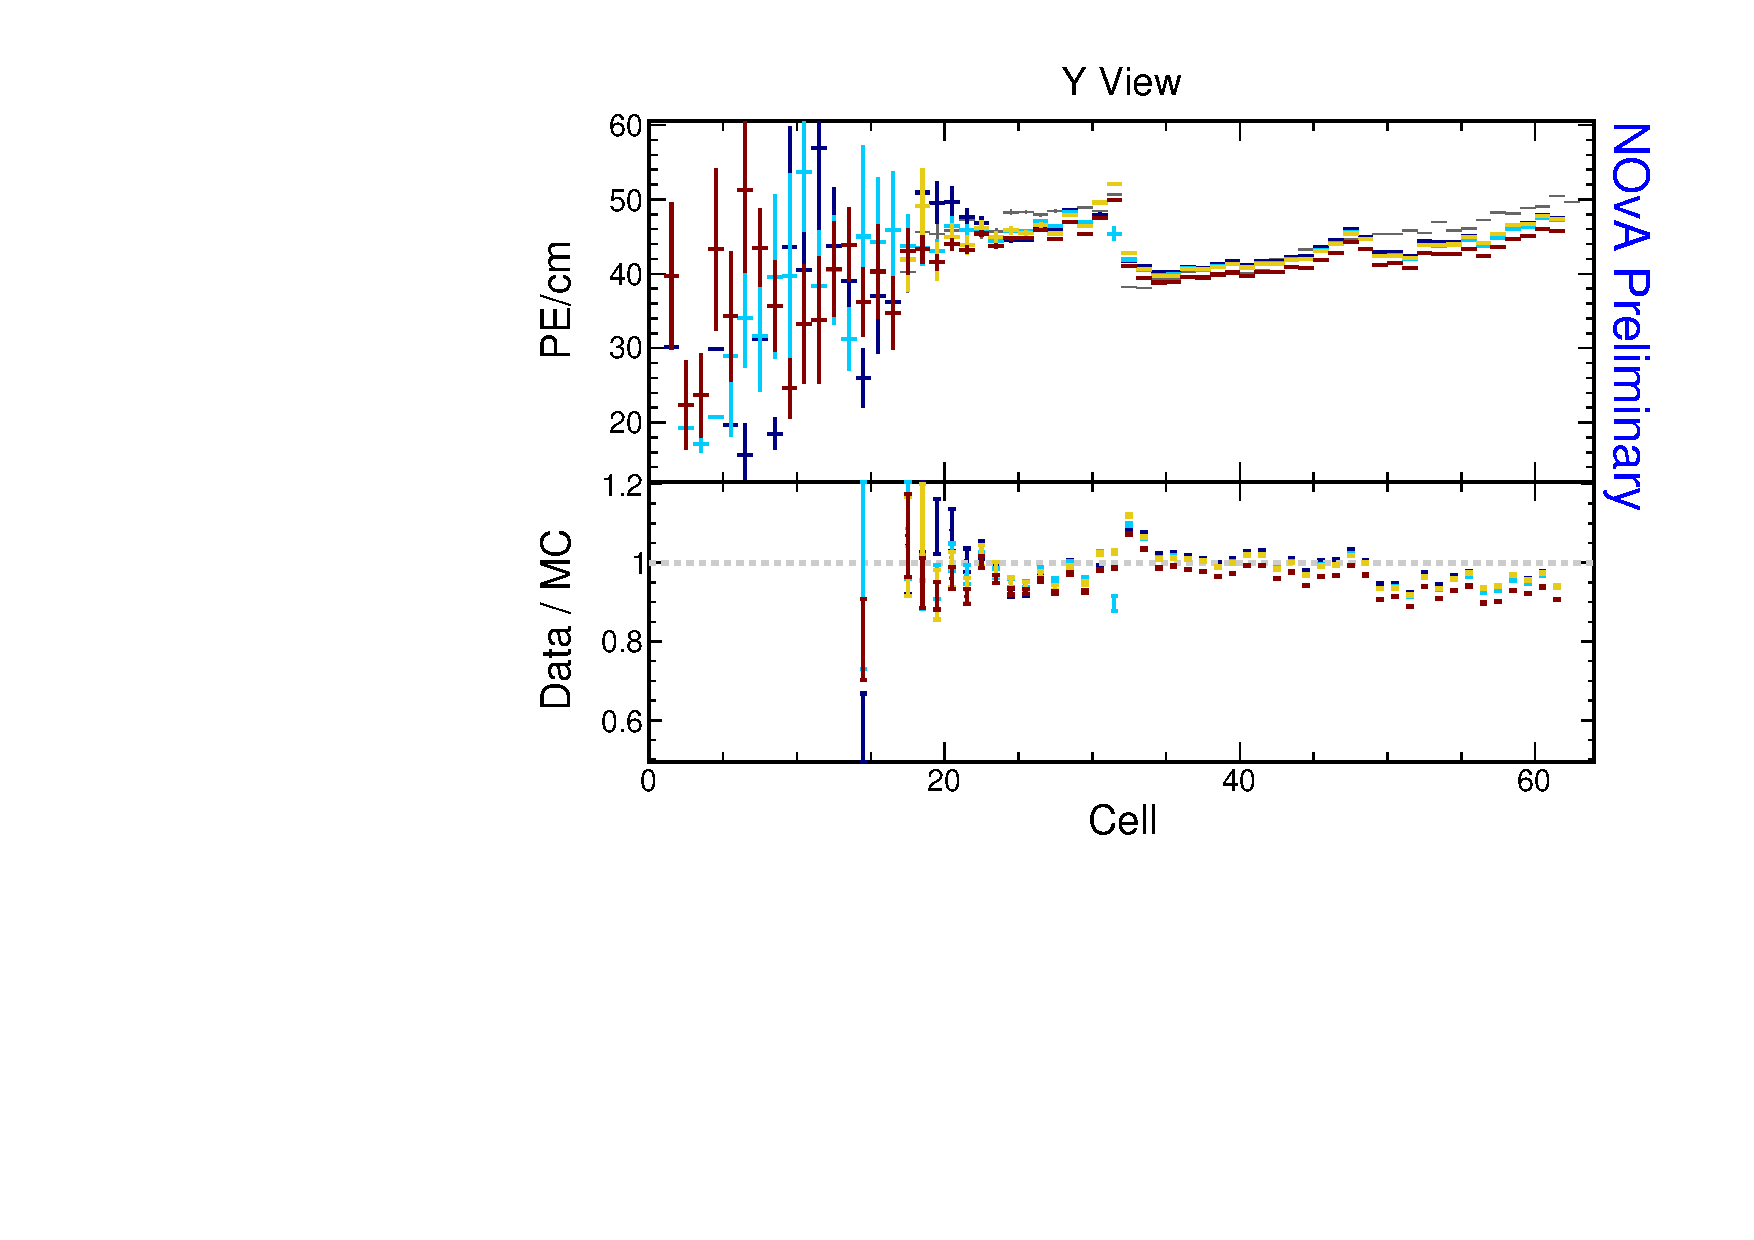
\includegraphics[width=\linewidth]{Plots/Calibana/pecm_cell_y.pdf}
  \end{subfigure}
  \begin{subfigure}{0.495\textwidth}
    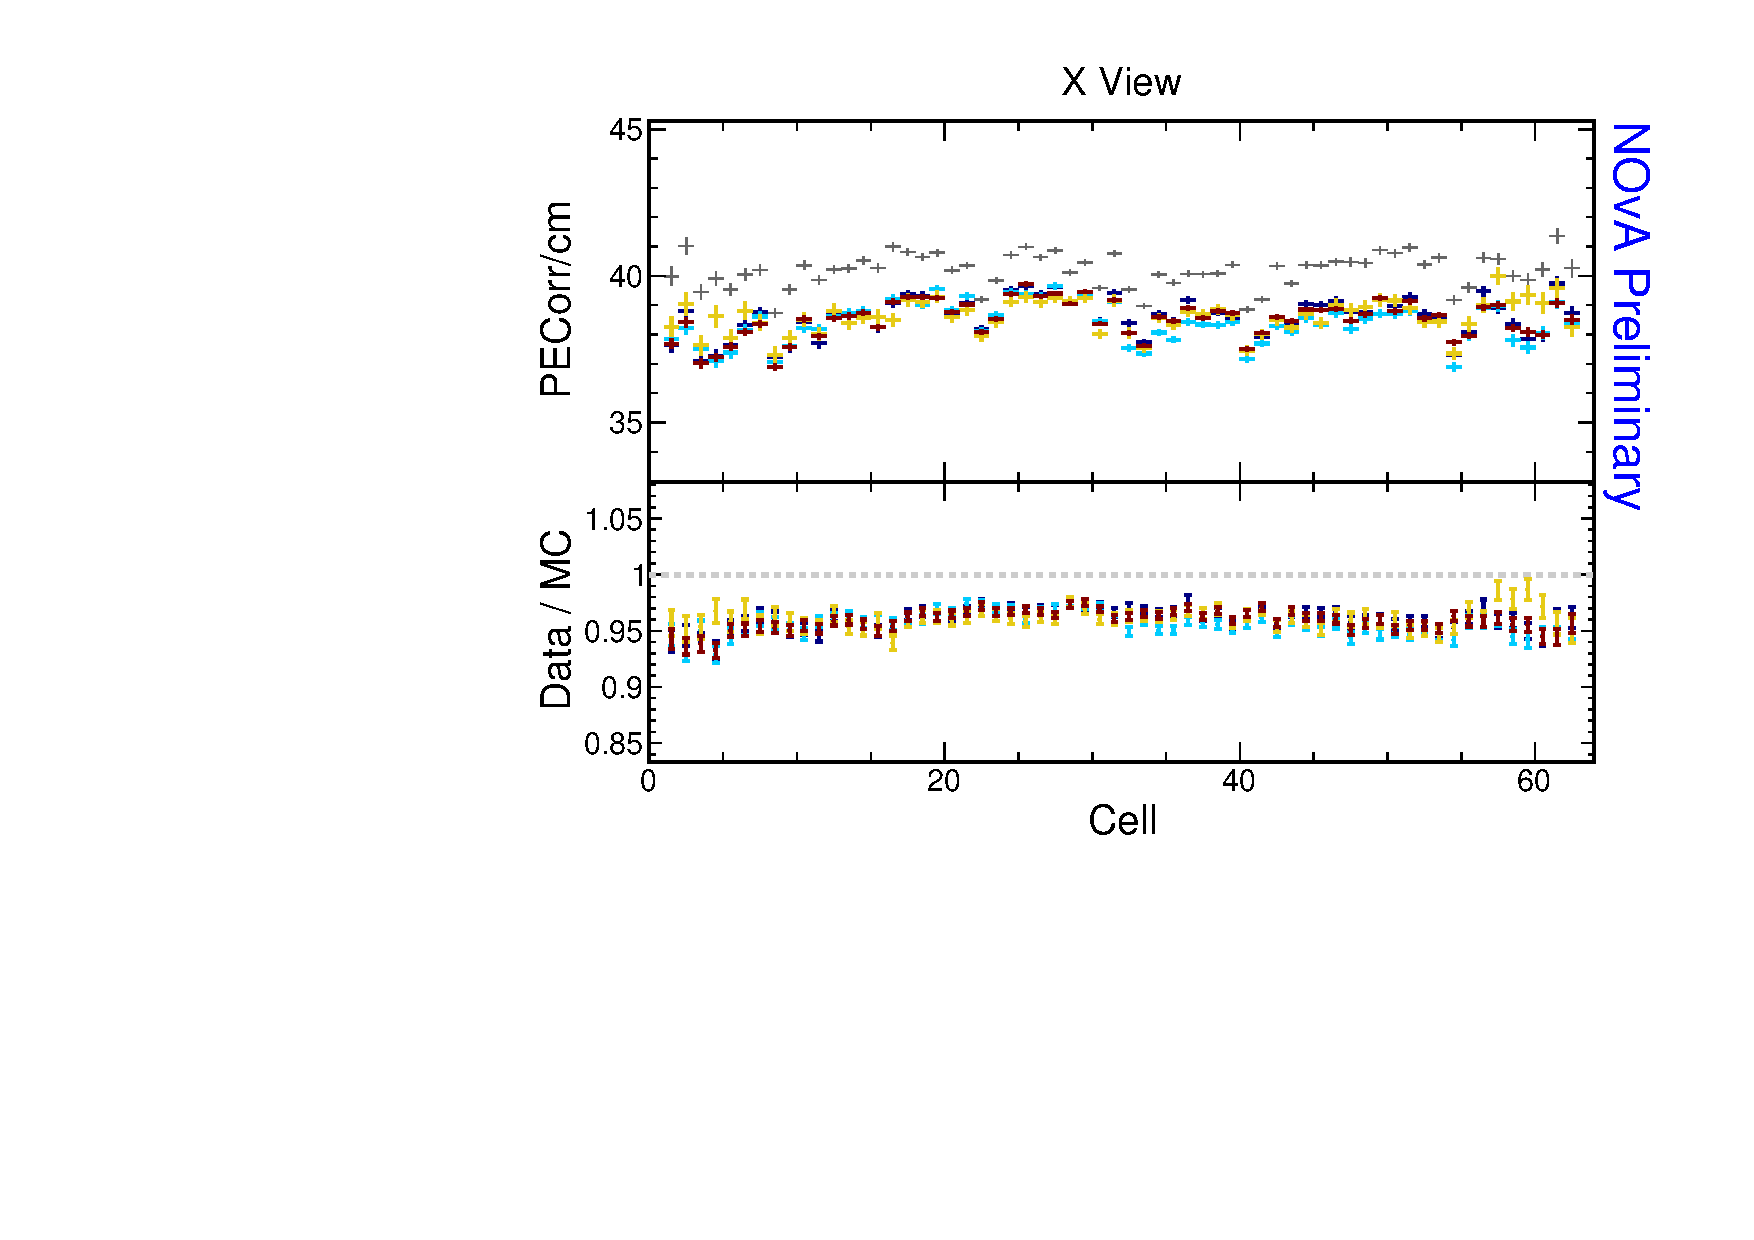
\includegraphics[width=\linewidth]{Plots/Calibana/pecorrcm_cell_x.pdf}
  \end{subfigure}
  \begin{subfigure}{0.495\textwidth}
    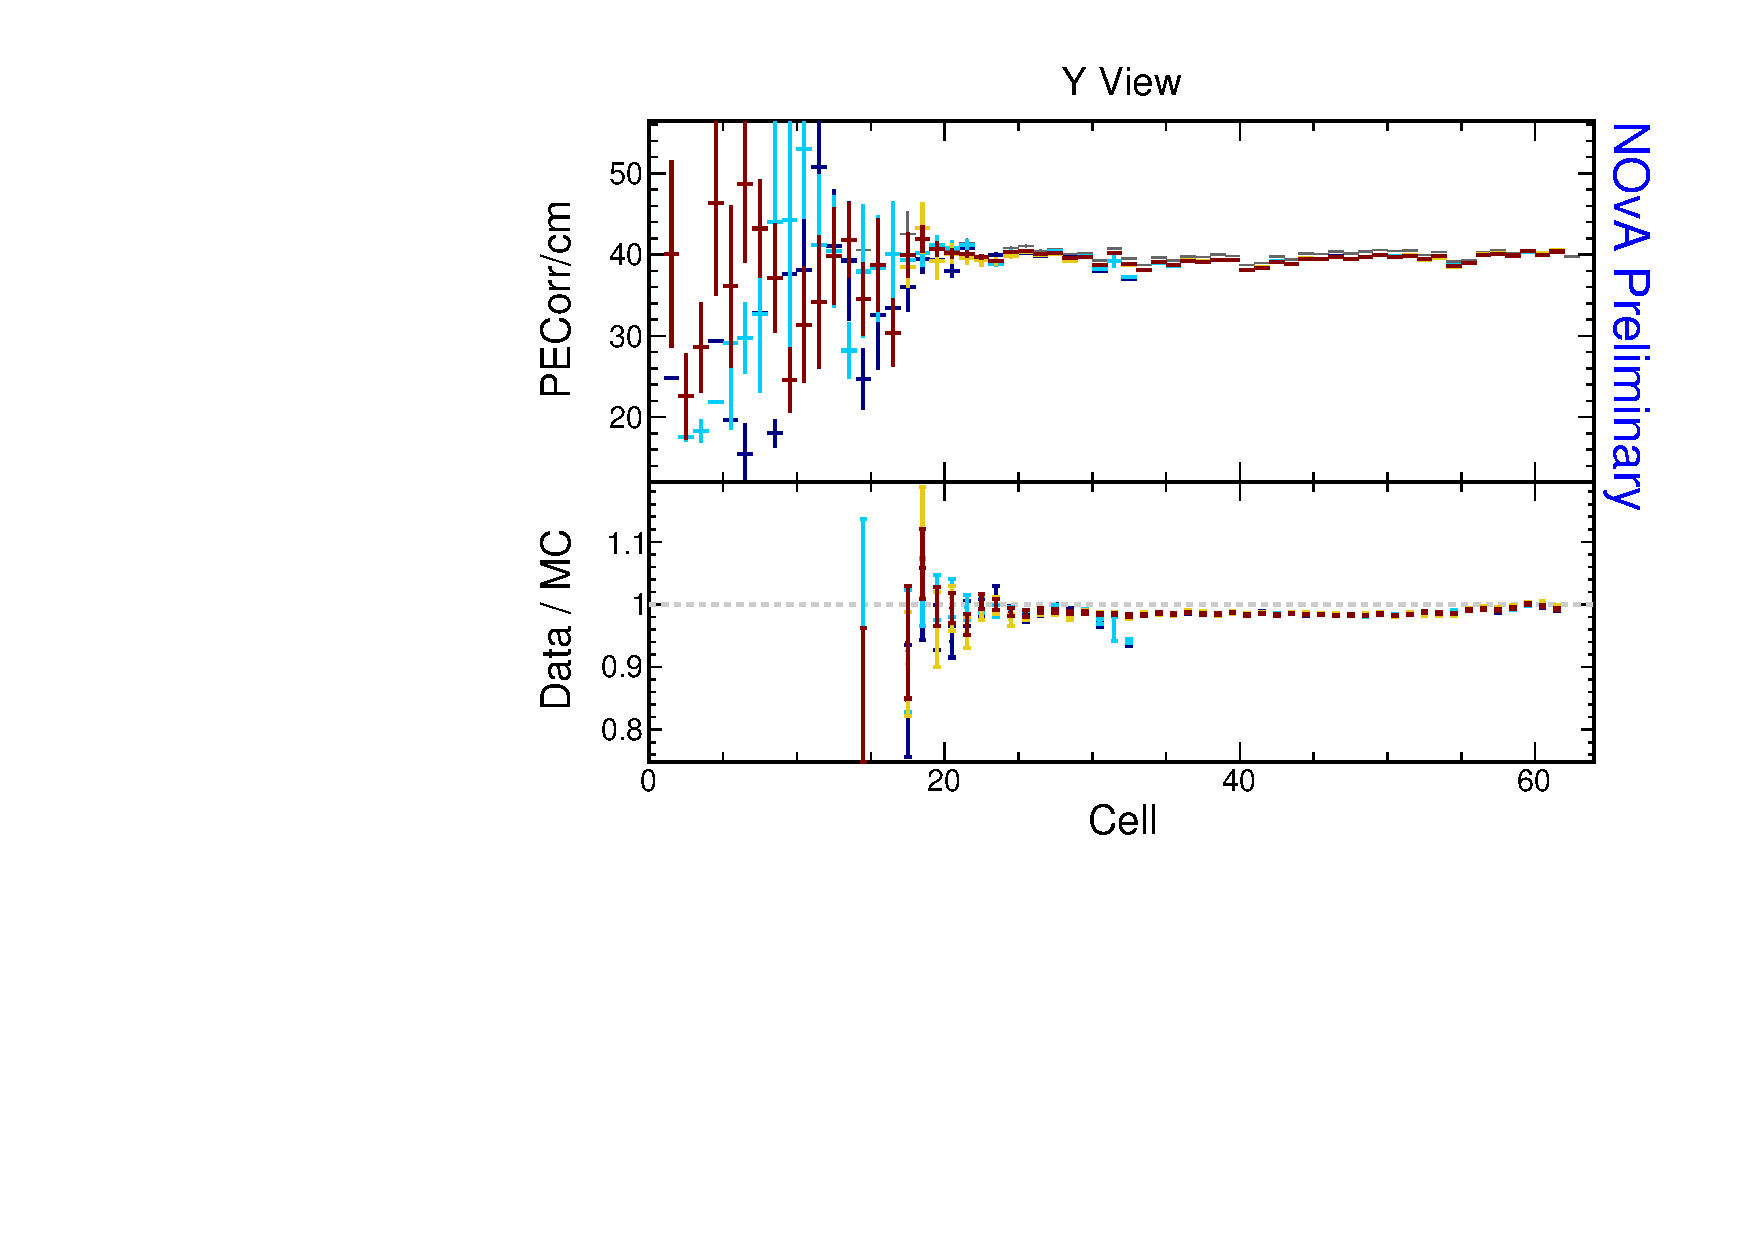
\includegraphics[width=\linewidth]{Plots/Calibana/pecorrcm_cell_y.pdf}
  \end{subfigure}
    \begin{subfigure}{0.495\textwidth}
    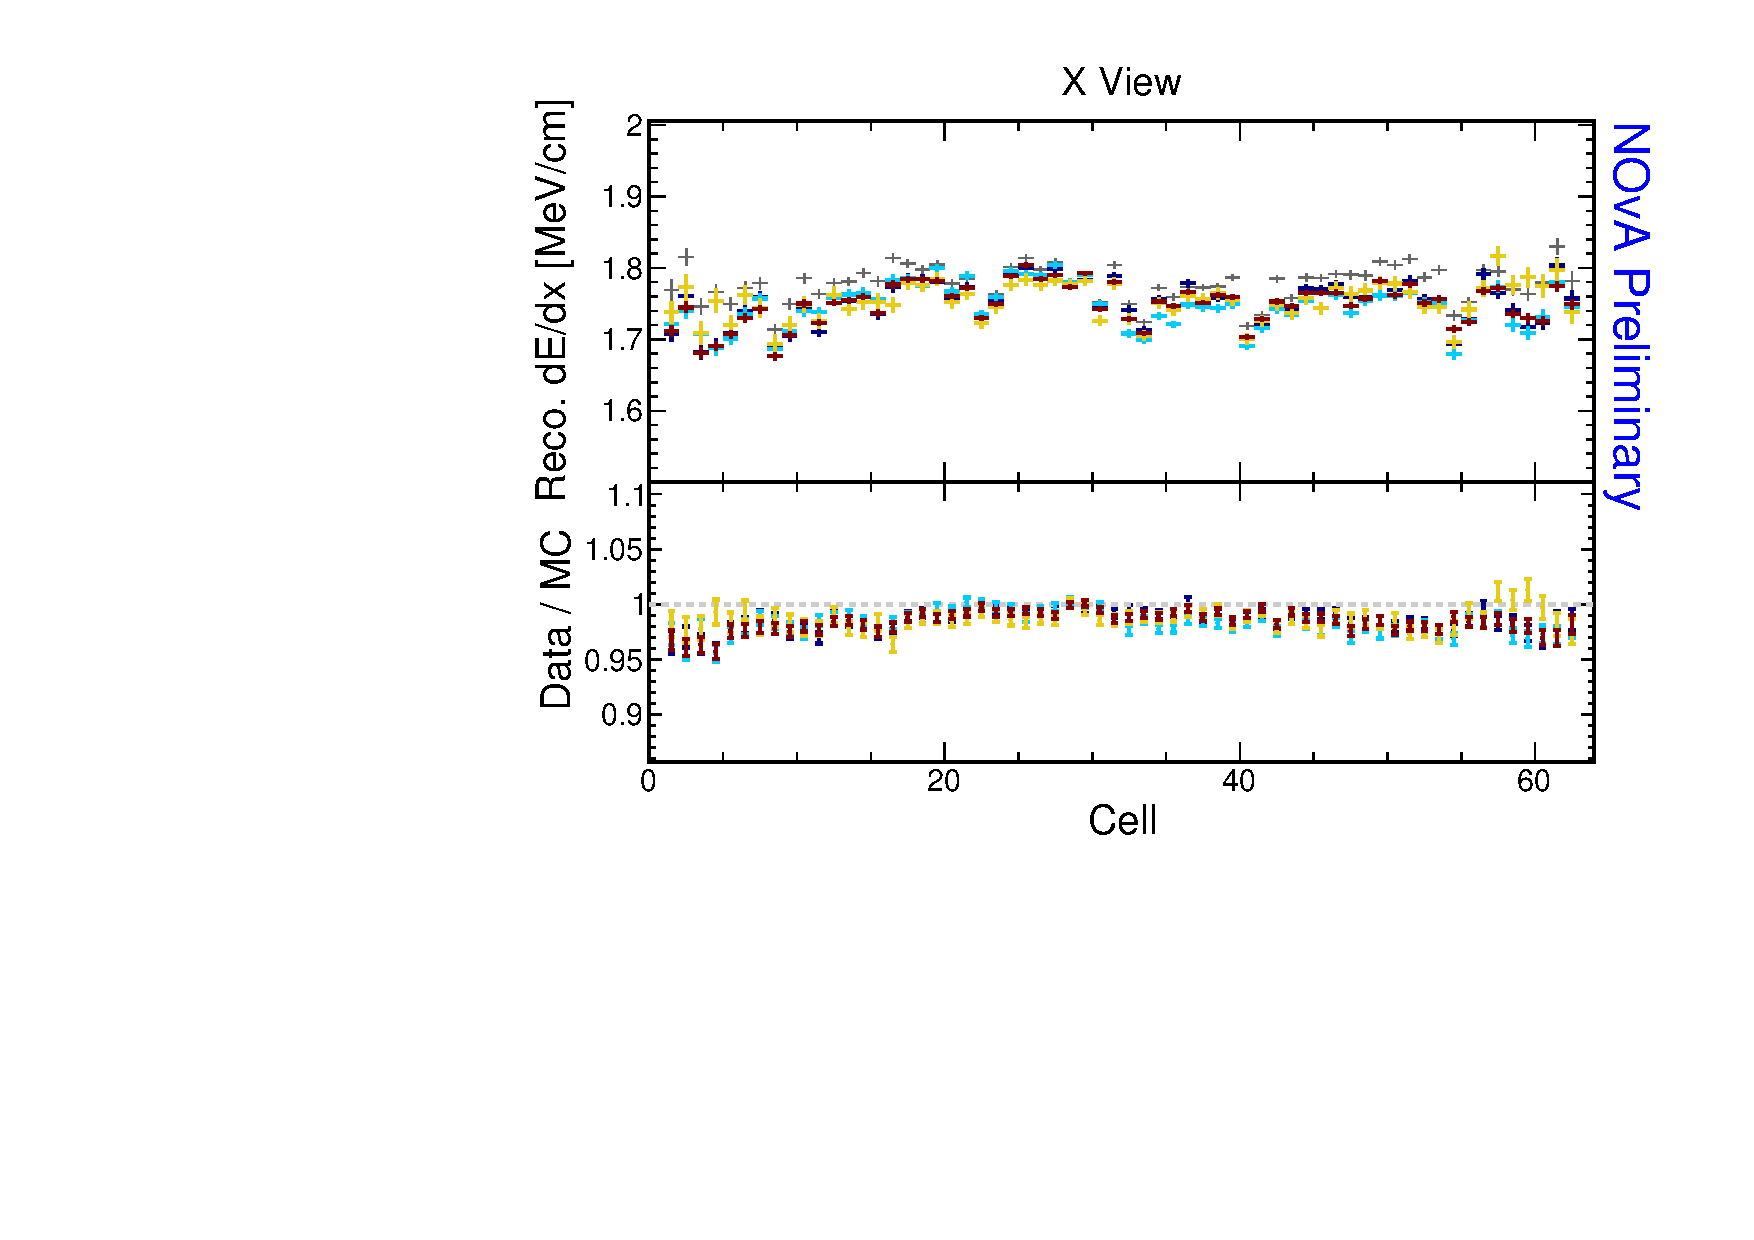
\includegraphics[width=\linewidth]{Plots/Calibana/recomevcm_cell_x.pdf}
  \end{subfigure}
  \begin{subfigure}{0.495\textwidth}
    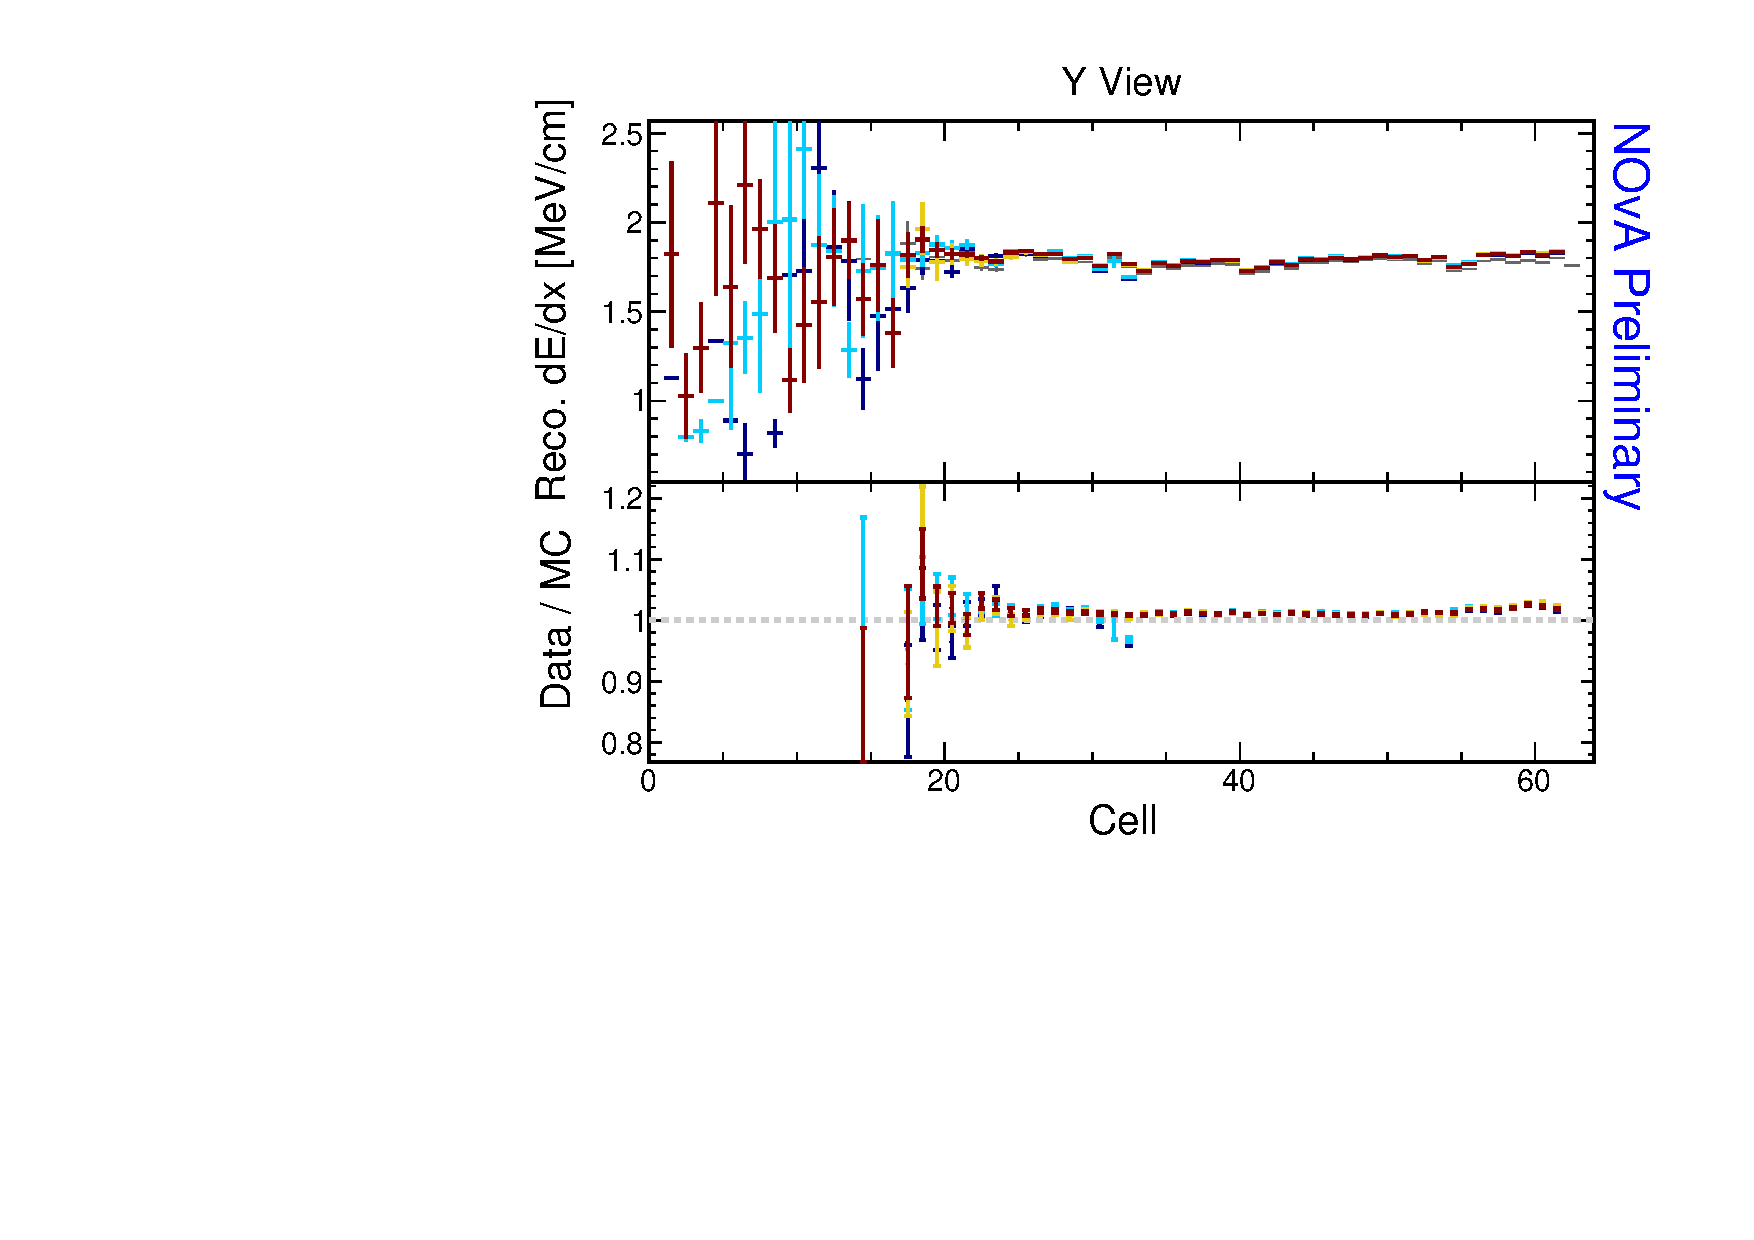
\includegraphics[width=\linewidth]{Plots/Calibana/recomevcm_cell_y.pdf}
  \end{subfigure}
  \caption[Energy deposition of stopping muons across cells]{Distributions of stopping muons within a 1-2 m track window from the end of their tracks across the cells for simulation (gray) and all the Test Beam data samples. The top row shows the energy deposition before any correction, middle row after relative calibration corrections and bottom row after full calibration corrections. The left column shows the X view (vertical planes) and right column the Y view (horizontal planes).}
  %\label{fig:AbsCalibCell1}
\end{figure}

\begin{figure}[!ht]
  \begin{subfigure}{\textwidth}
  \centering
    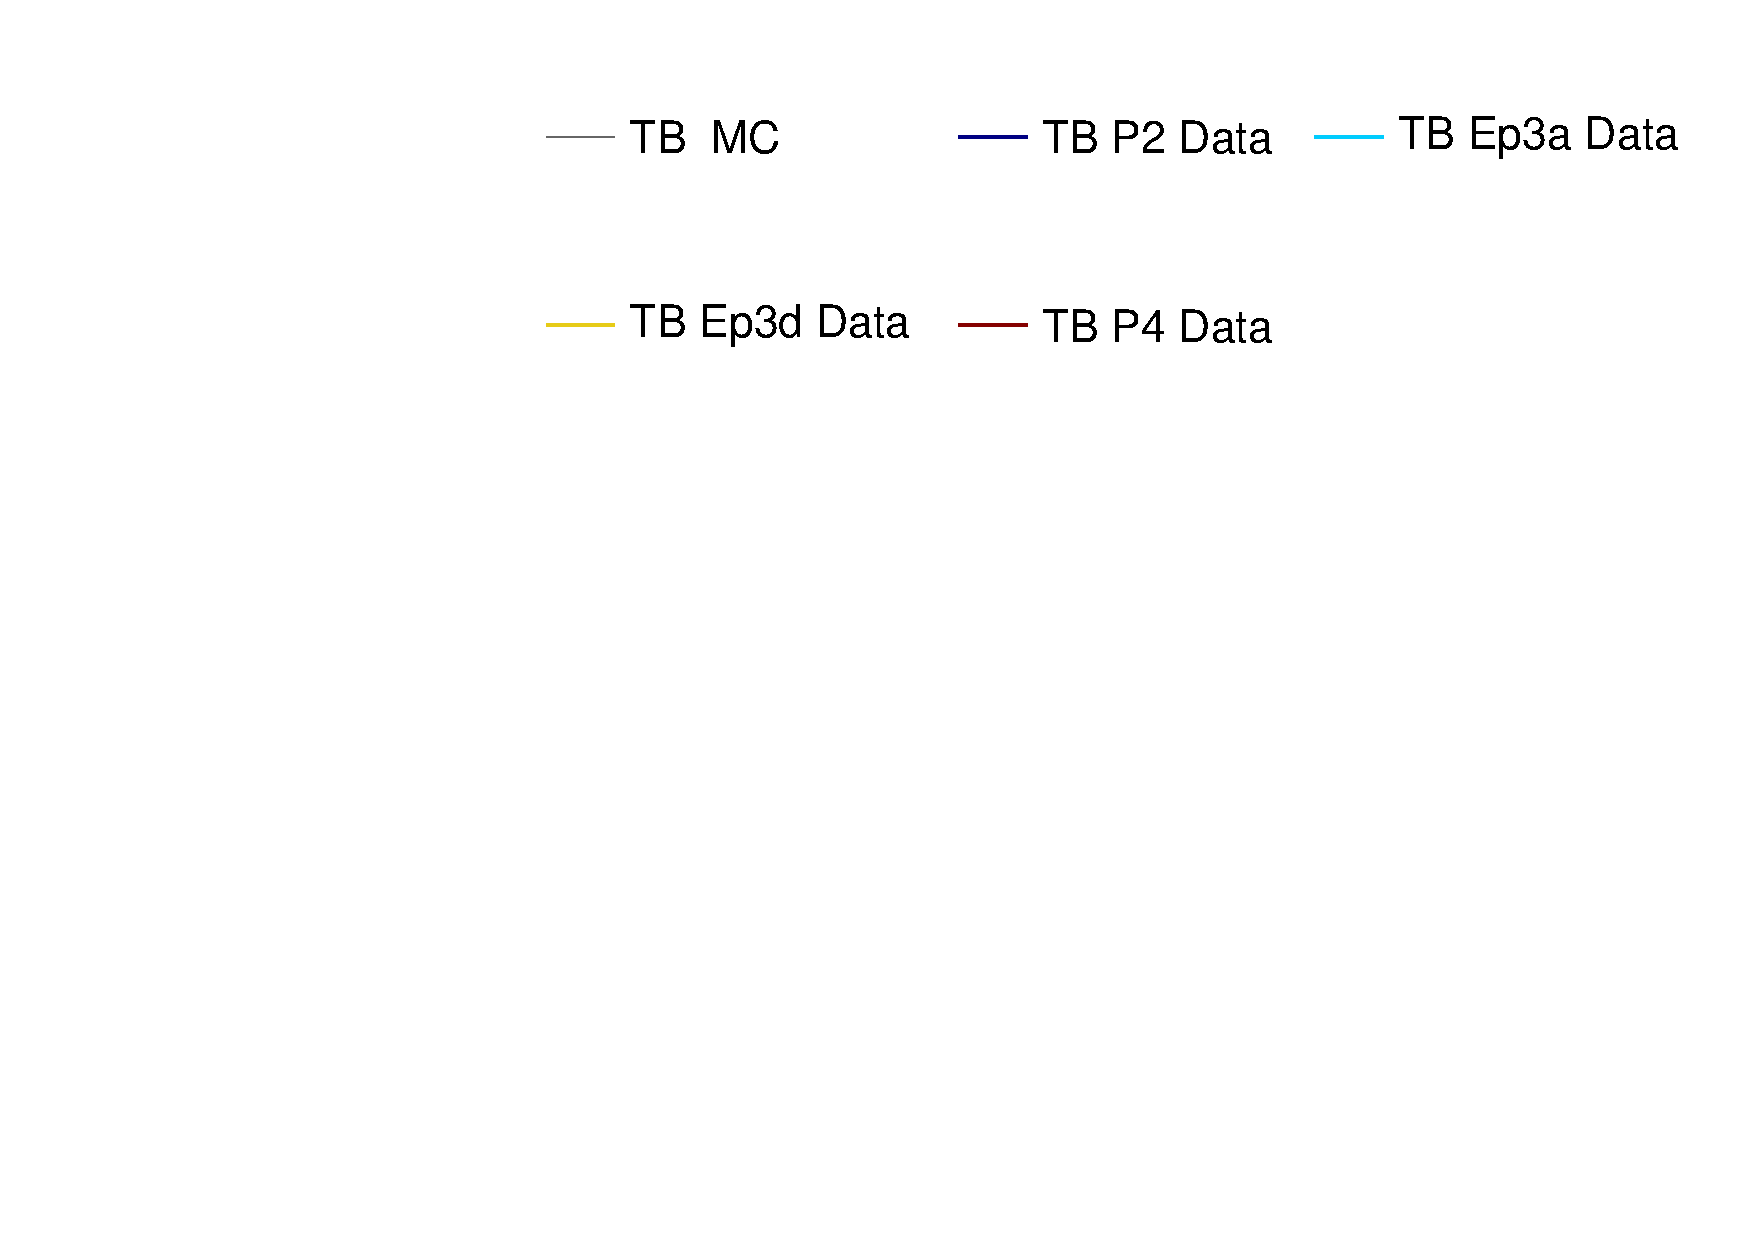
\includegraphics[height=0.2\linewidth]{Plots/Calibana/legend.pdf}
  \end{subfigure}
  \vspace*{2mm}

  \begin{subfigure}{0.495\textwidth}
    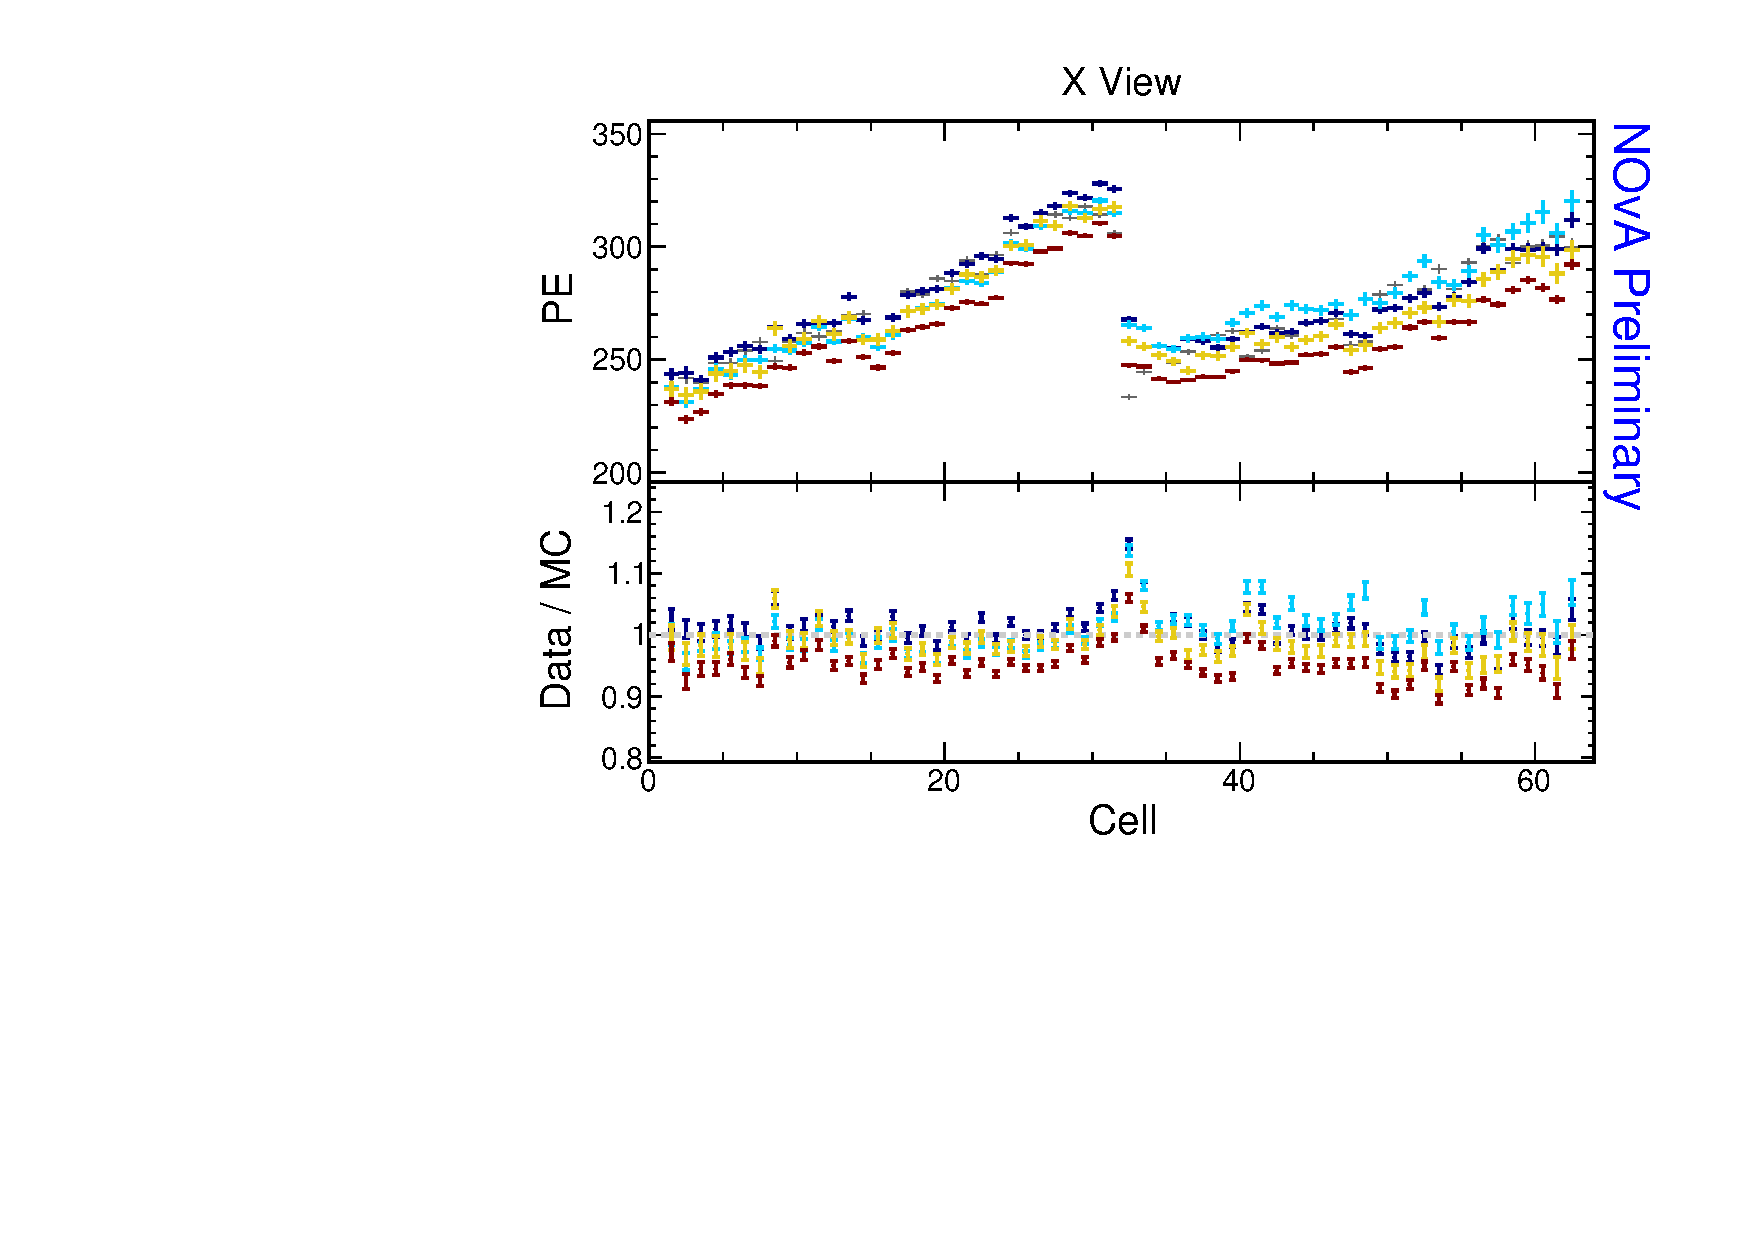
\includegraphics[width=\linewidth]{Plots/Calibana/pe_cell_x.pdf}
  \end{subfigure}
  \begin{subfigure}{0.495\textwidth}
    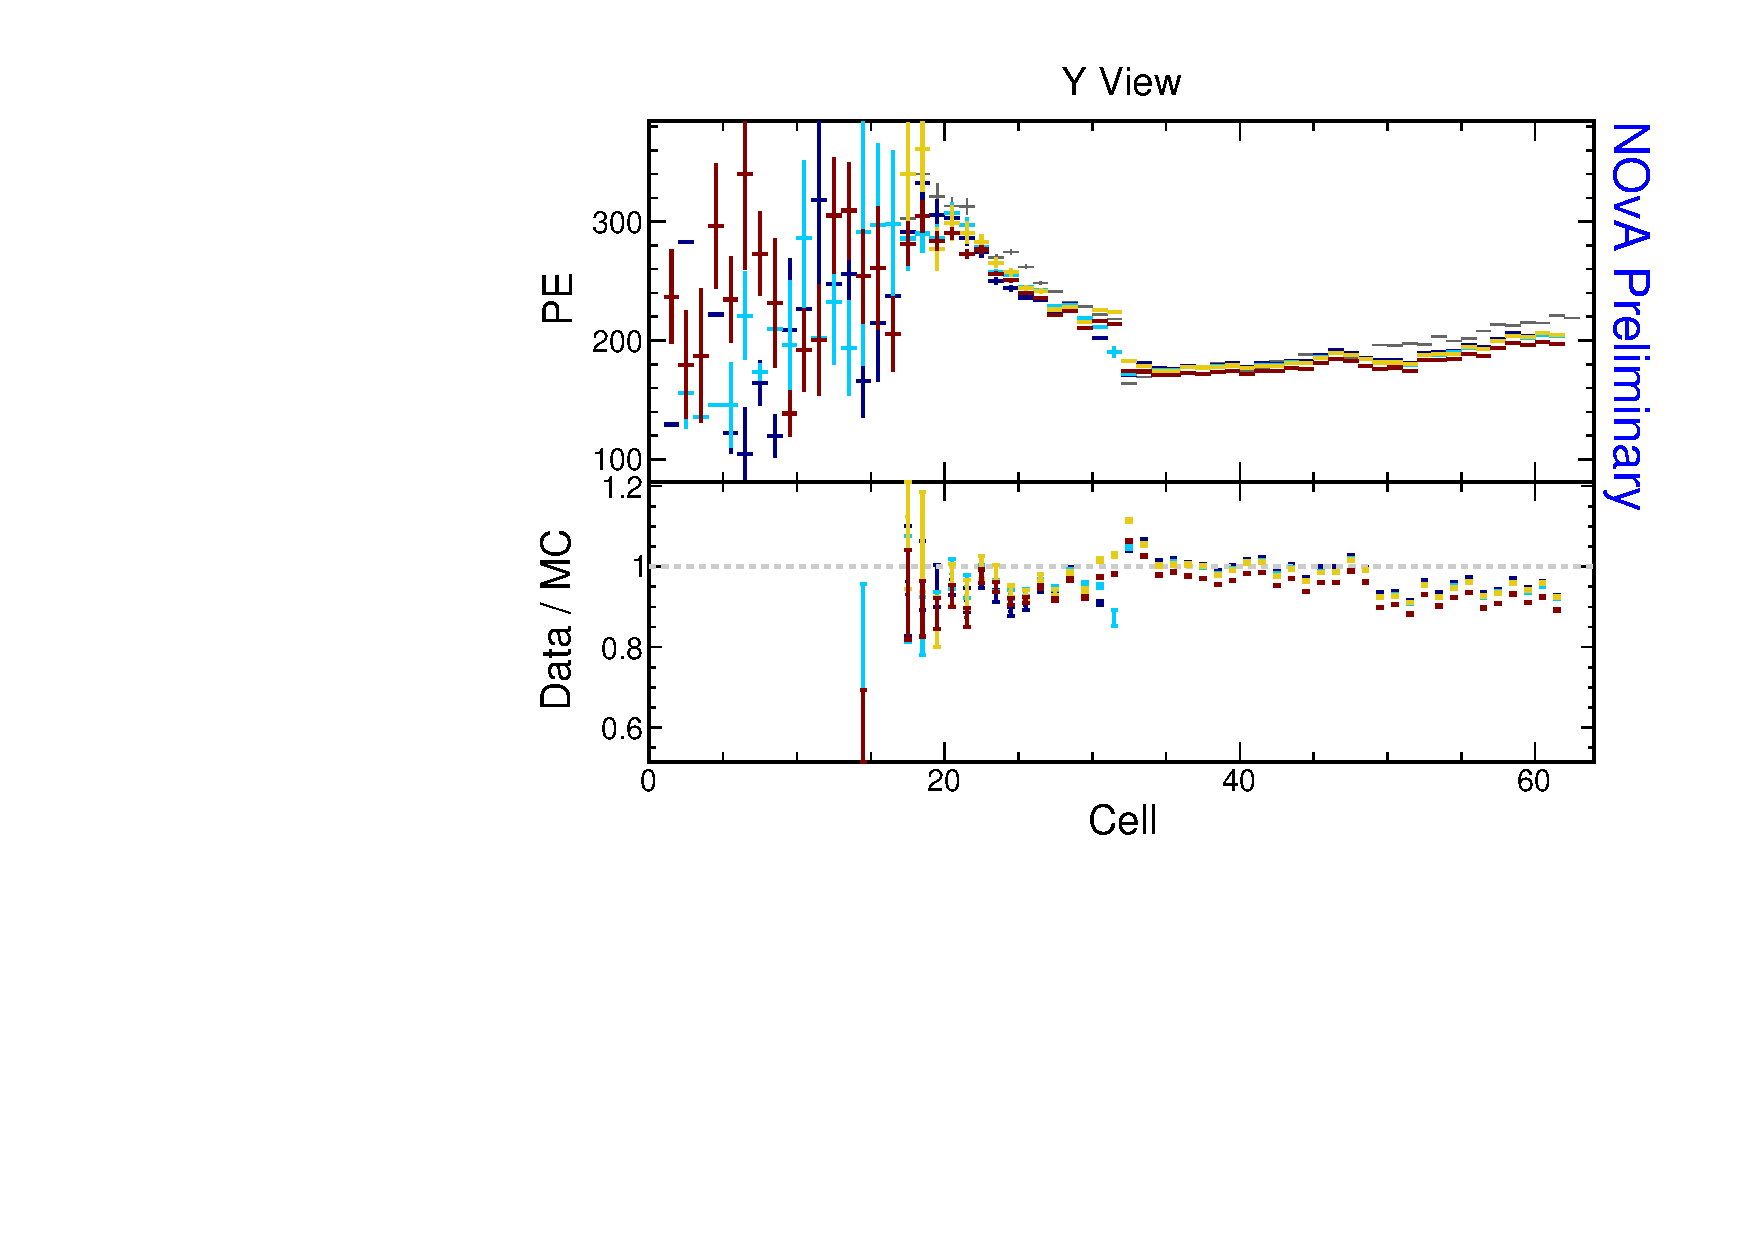
\includegraphics[width=\linewidth]{Plots/Calibana/pe_cell_y.pdf}
  \end{subfigure}
  \begin{subfigure}{0.495\textwidth}
    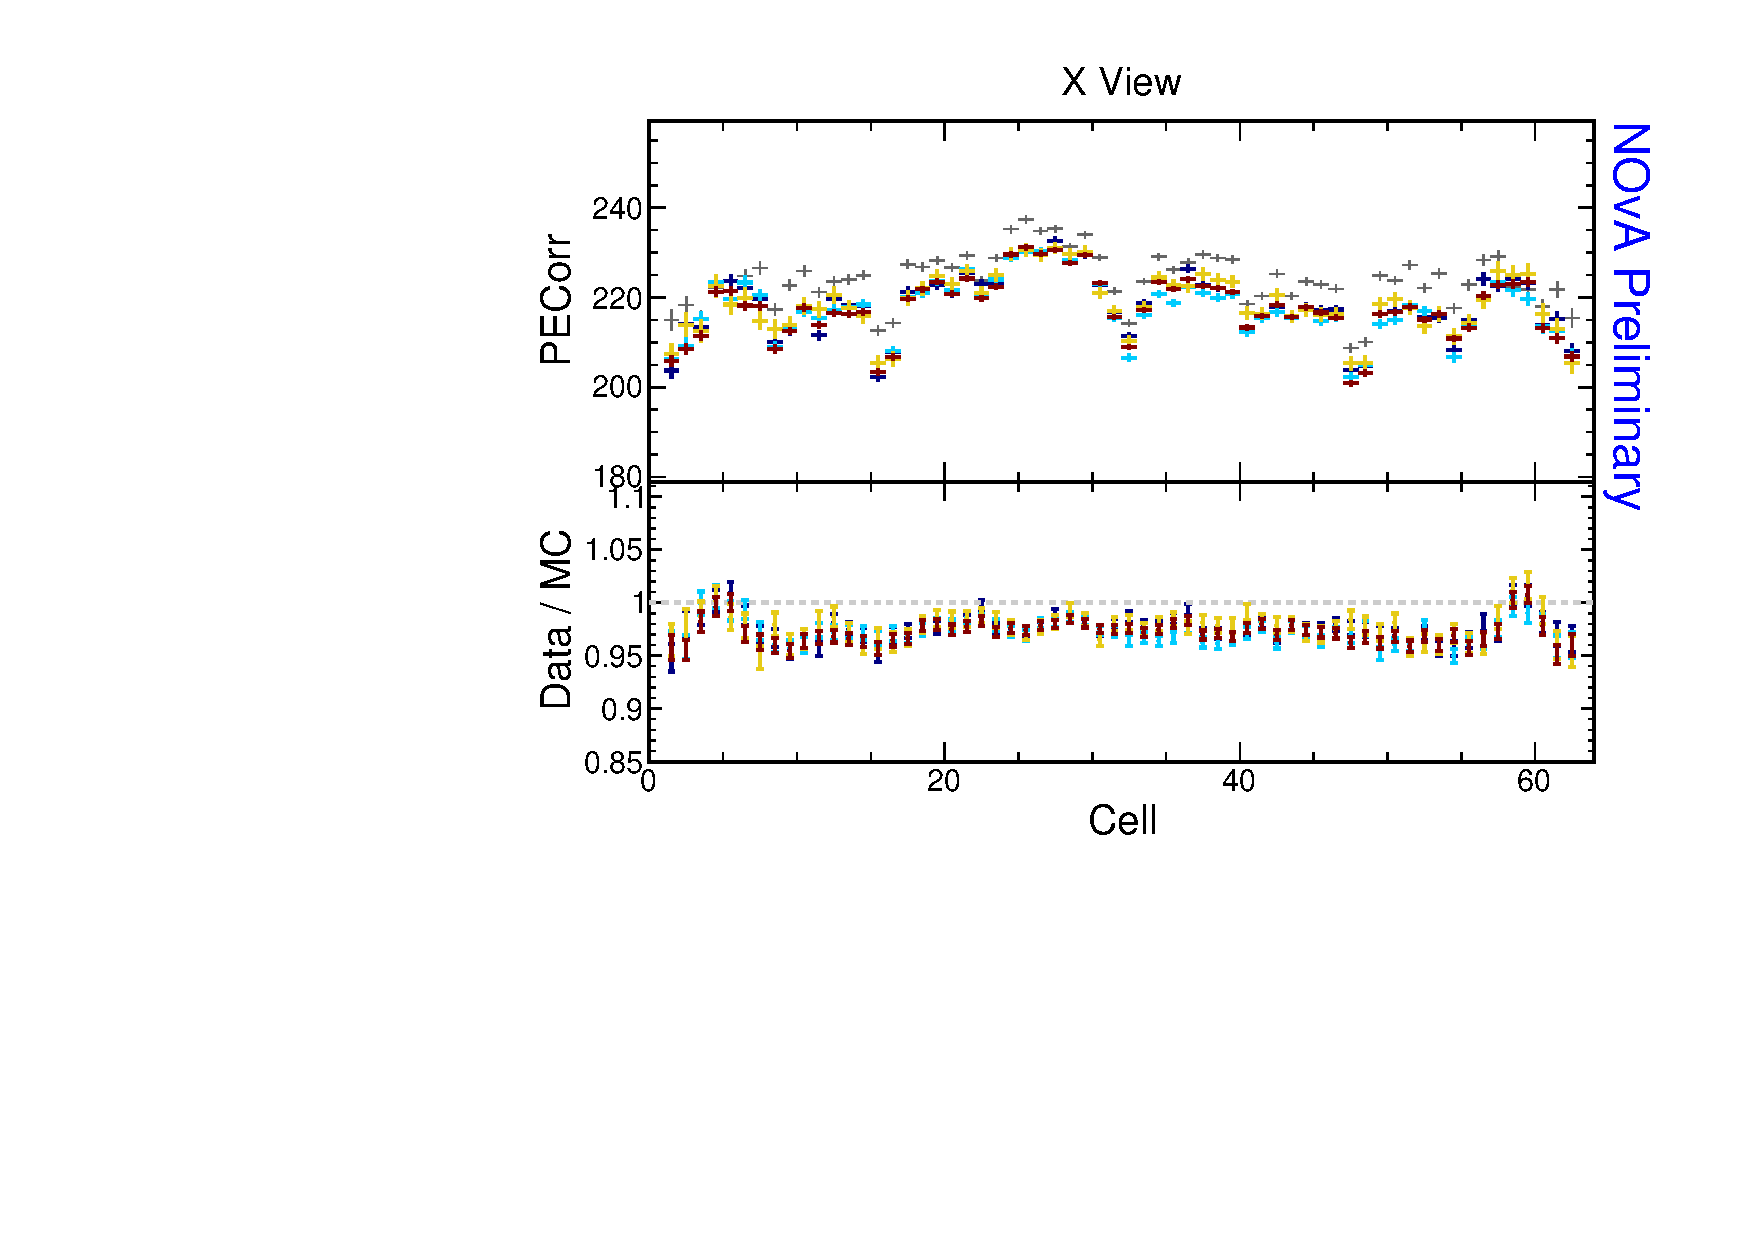
\includegraphics[width=\linewidth]{Plots/Calibana/pecorr_cell_x.pdf}
  \end{subfigure}
  \begin{subfigure}{0.495\textwidth}
    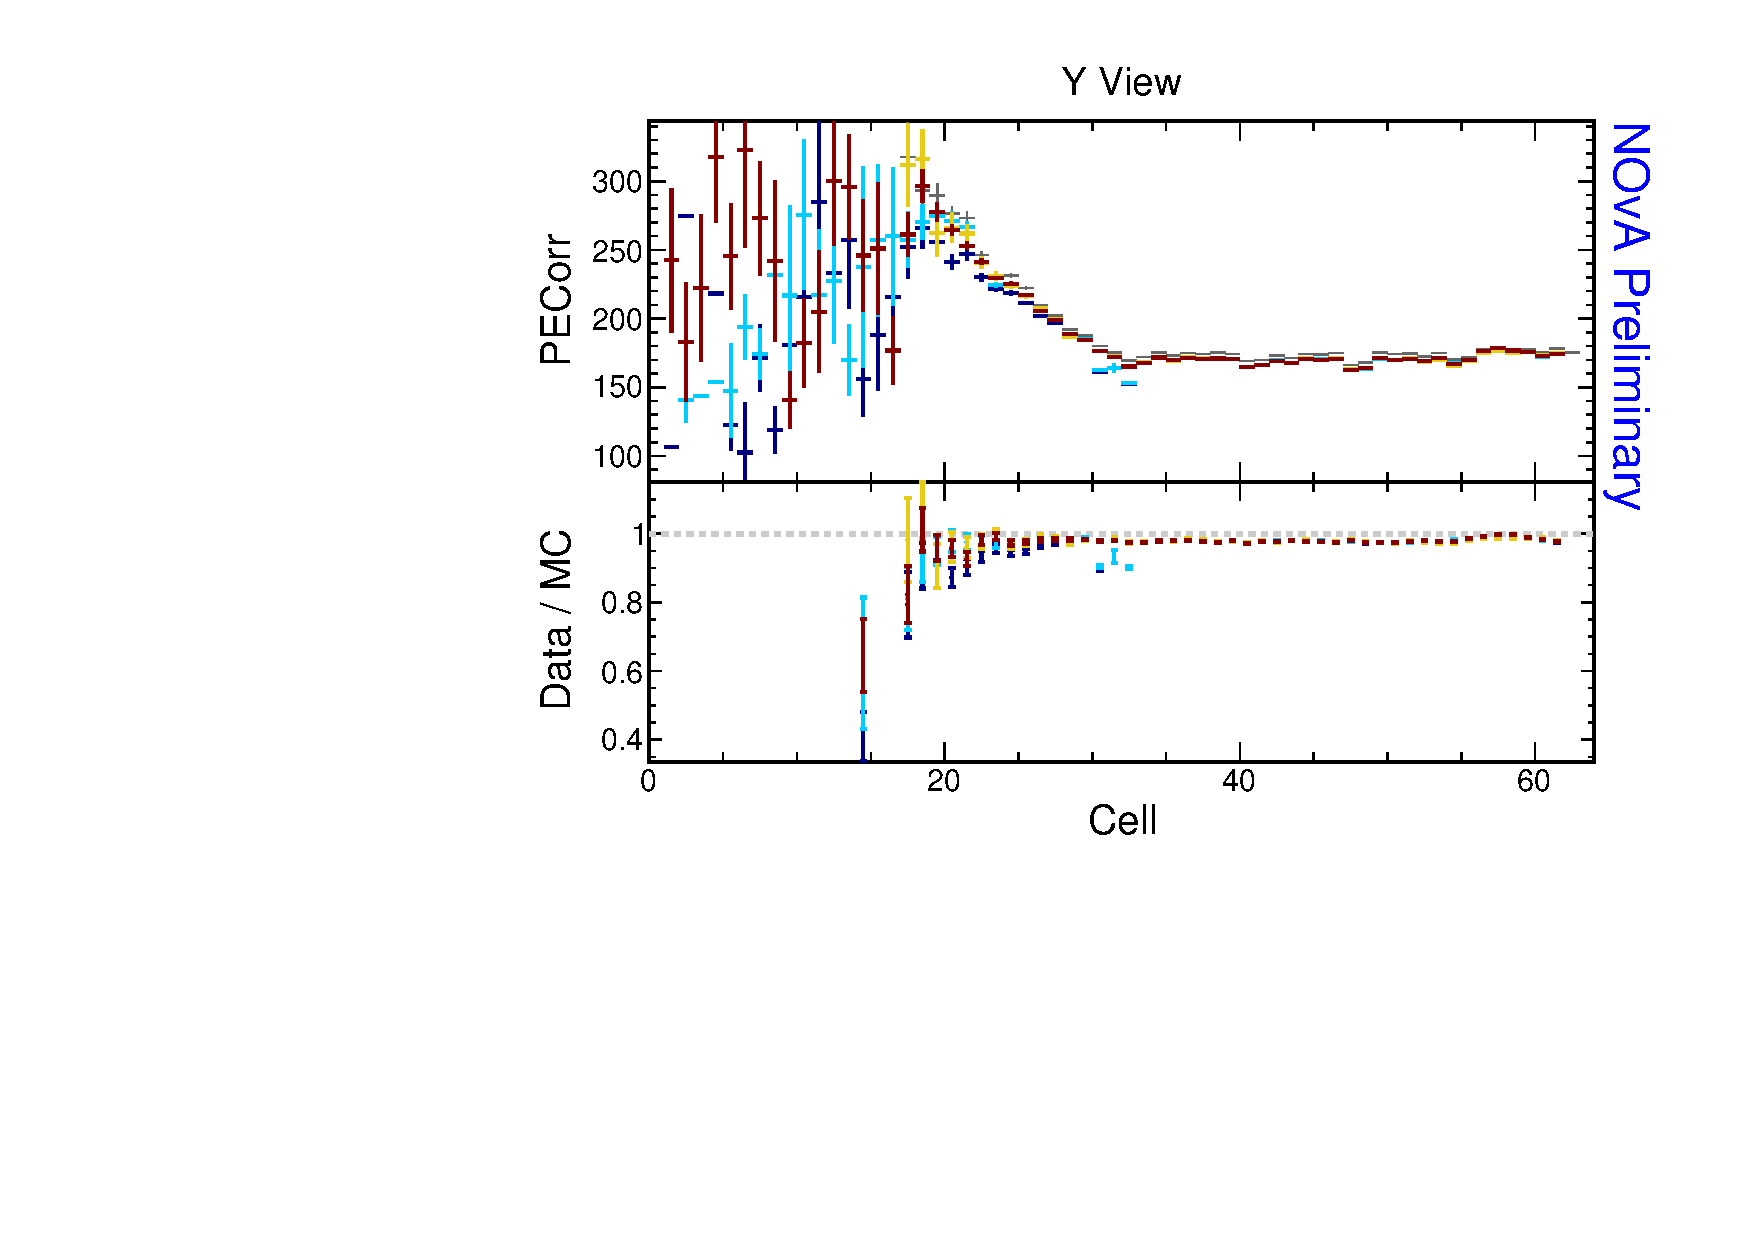
\includegraphics[width=\linewidth]{Plots/Calibana/pecorr_cell_y.pdf}
  \end{subfigure}
  \begin{subfigure}{0.495\textwidth}
    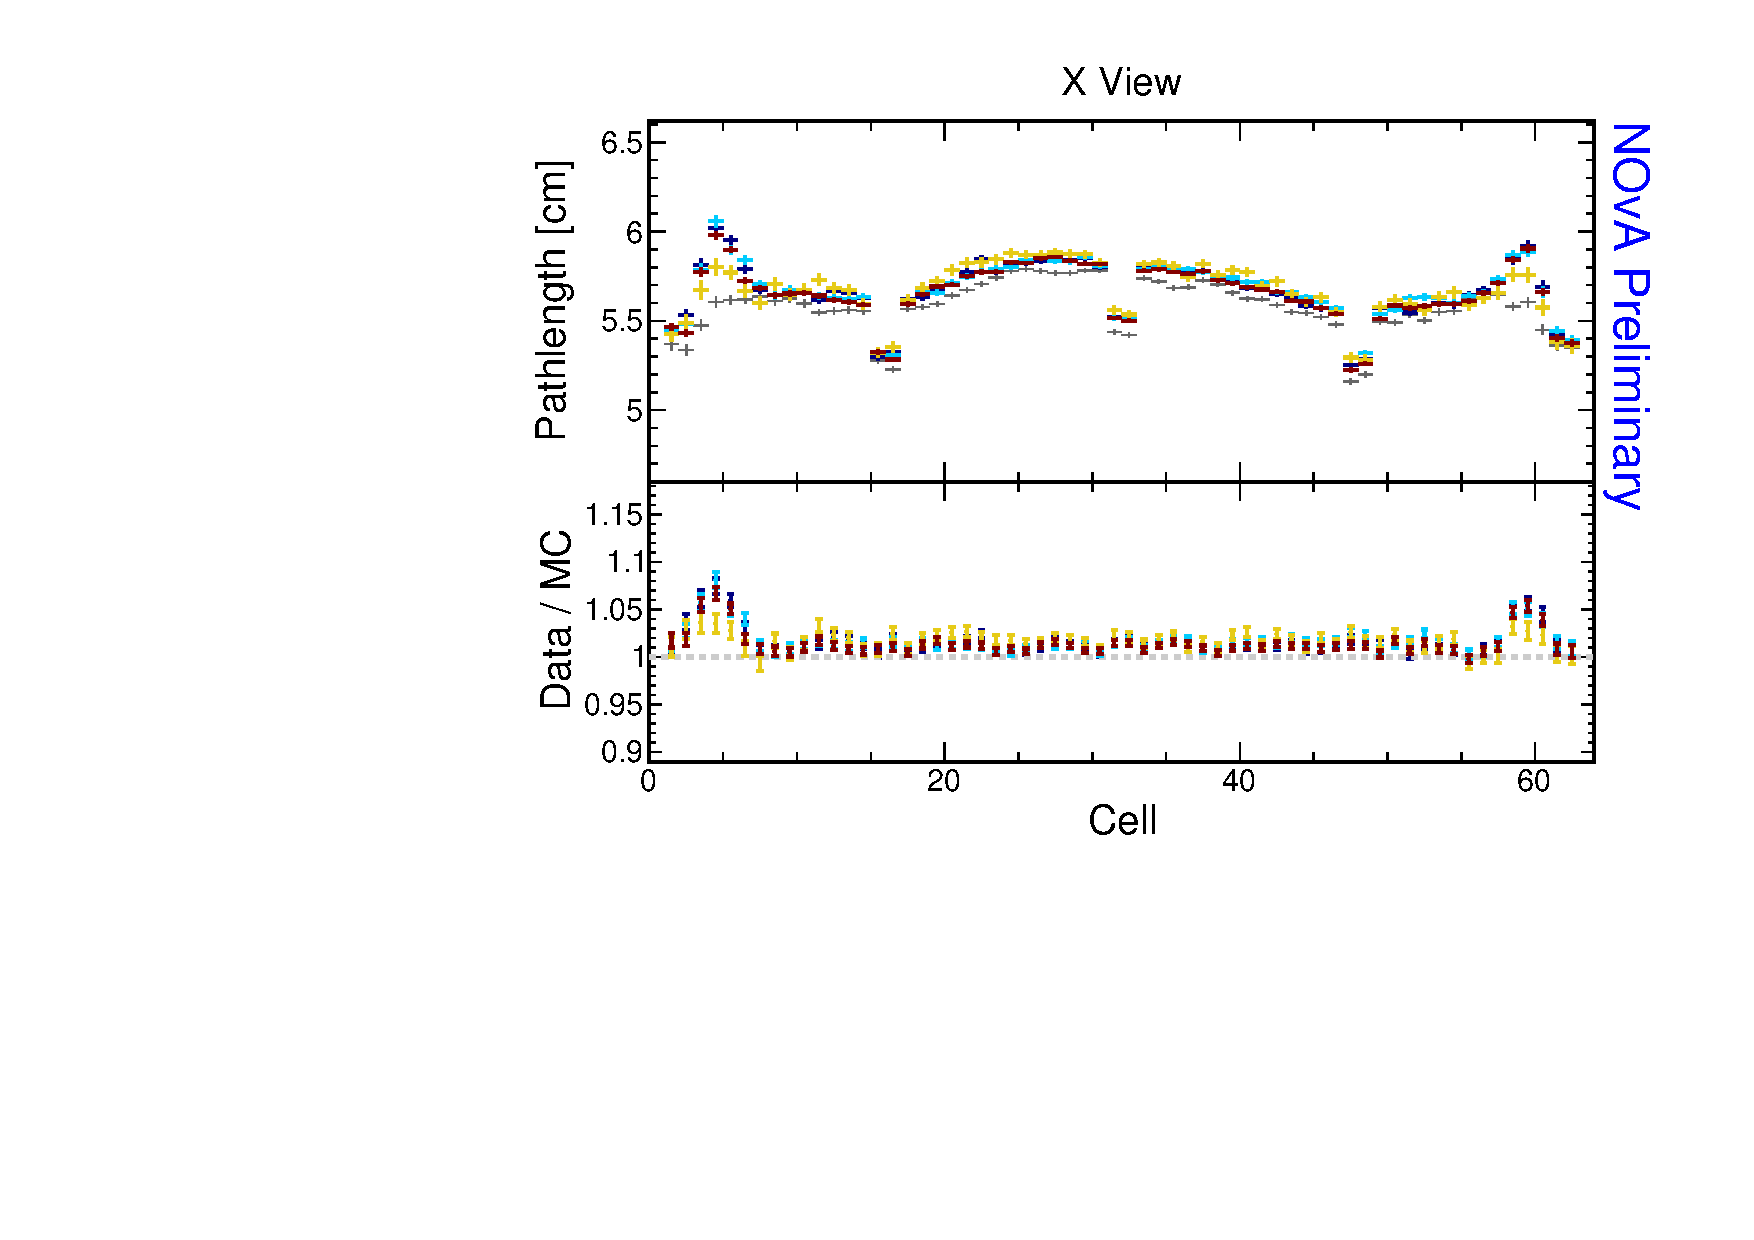
\includegraphics[width=\linewidth]{Plots/Calibana/cm_cell_x.pdf}
  \end{subfigure}
  \begin{subfigure}{0.495\textwidth}
    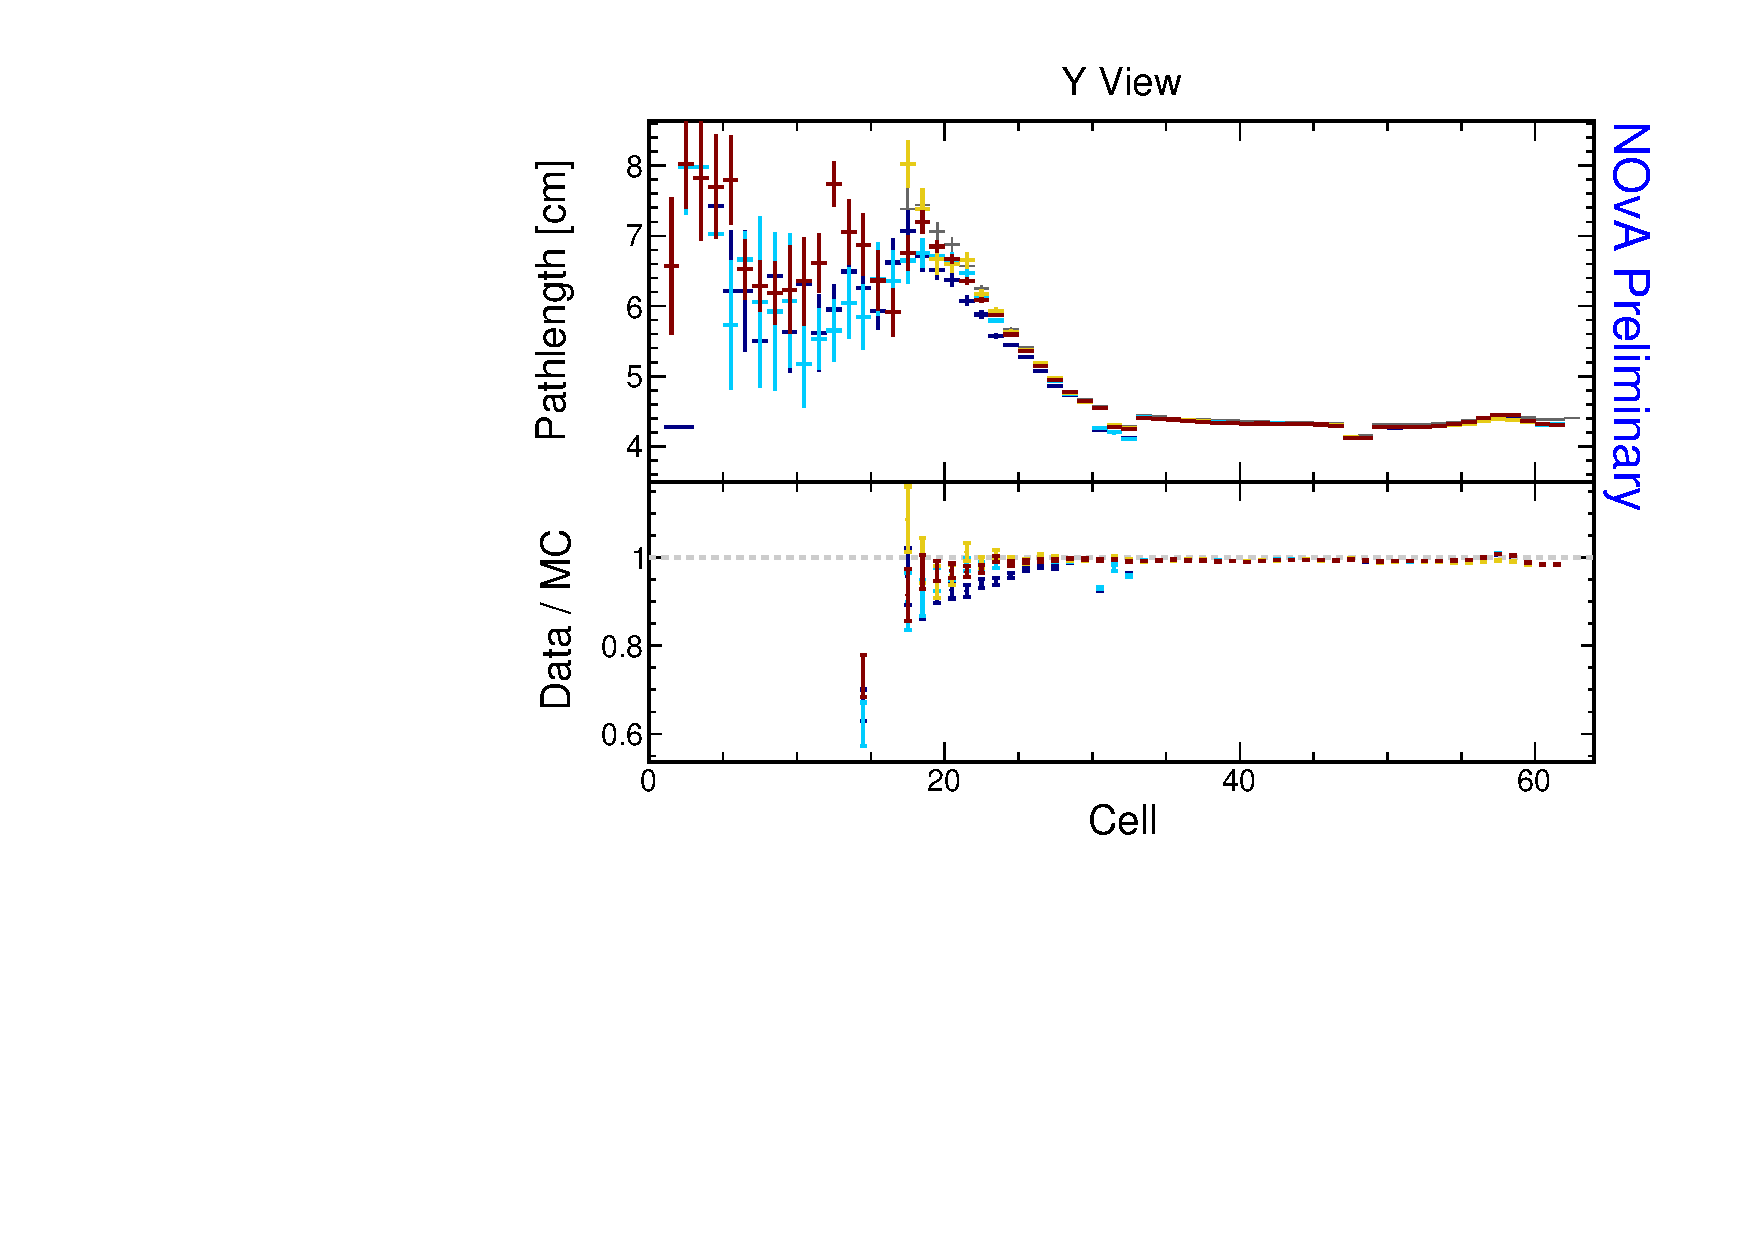
\includegraphics[width=\linewidth]{Plots/Calibana/cm_cell_y.pdf}
  \end{subfigure}
  \caption[Calibration variables of stopping muons across cells]{Distributions of stopping muons within a 1-2 m track window from the end of their tracks across the detector cells for simulation (gray) and all the Test Beam data samples. The top row shows the number of recorded photo electrons before any corrections, middle row shows the same after relative calibration corrections and bottom row shows the path length through the cell. The left column shows the X view (vertical planes) and right column the Y view (horizontal planes).}
  %\label{fig:AbsCalibCell2}
\end{figure}

\begin{figure}[!ht]
  \begin{subfigure}{\textwidth}
  \centering
    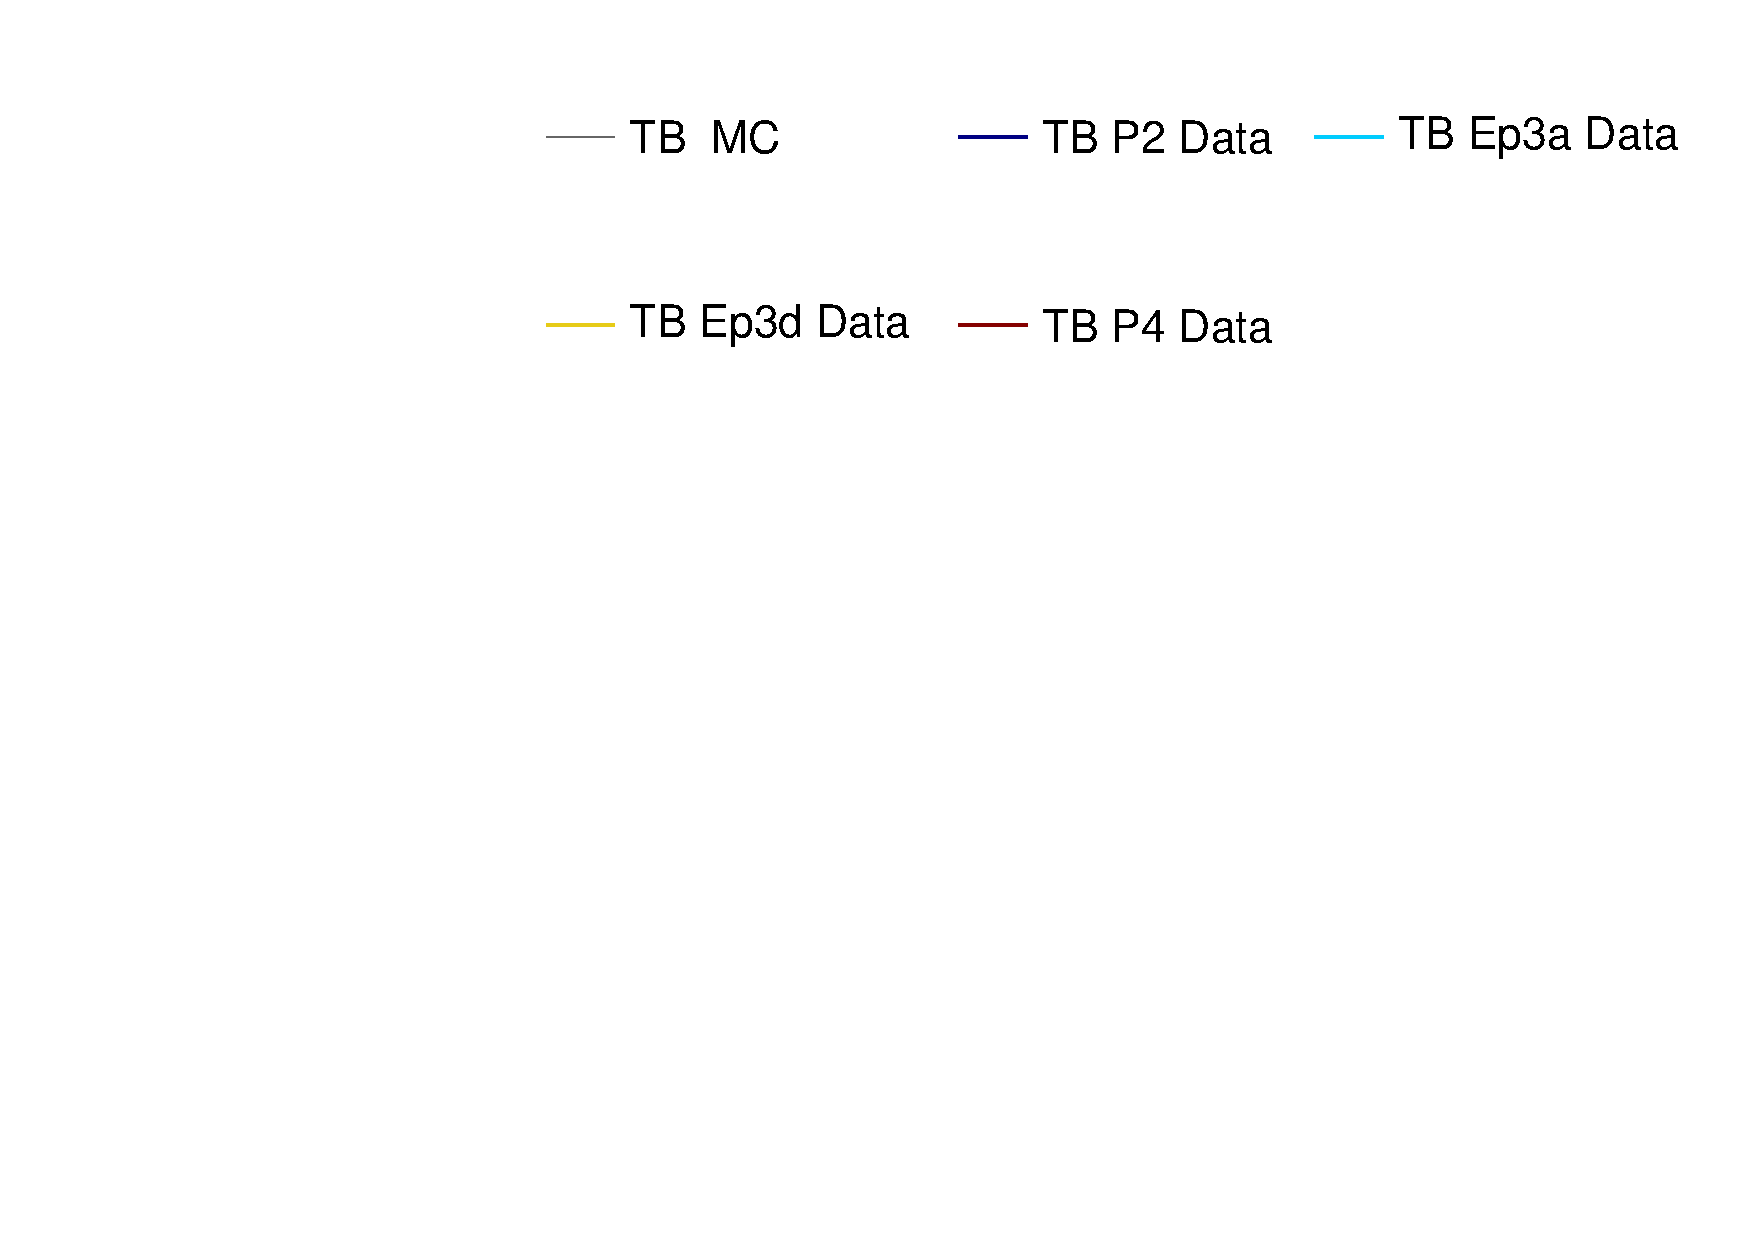
\includegraphics[height=0.2\linewidth]{Plots/Calibana/legend.pdf}
  \end{subfigure}
  \vspace*{2mm}

  \begin{subfigure}{0.495\textwidth}
    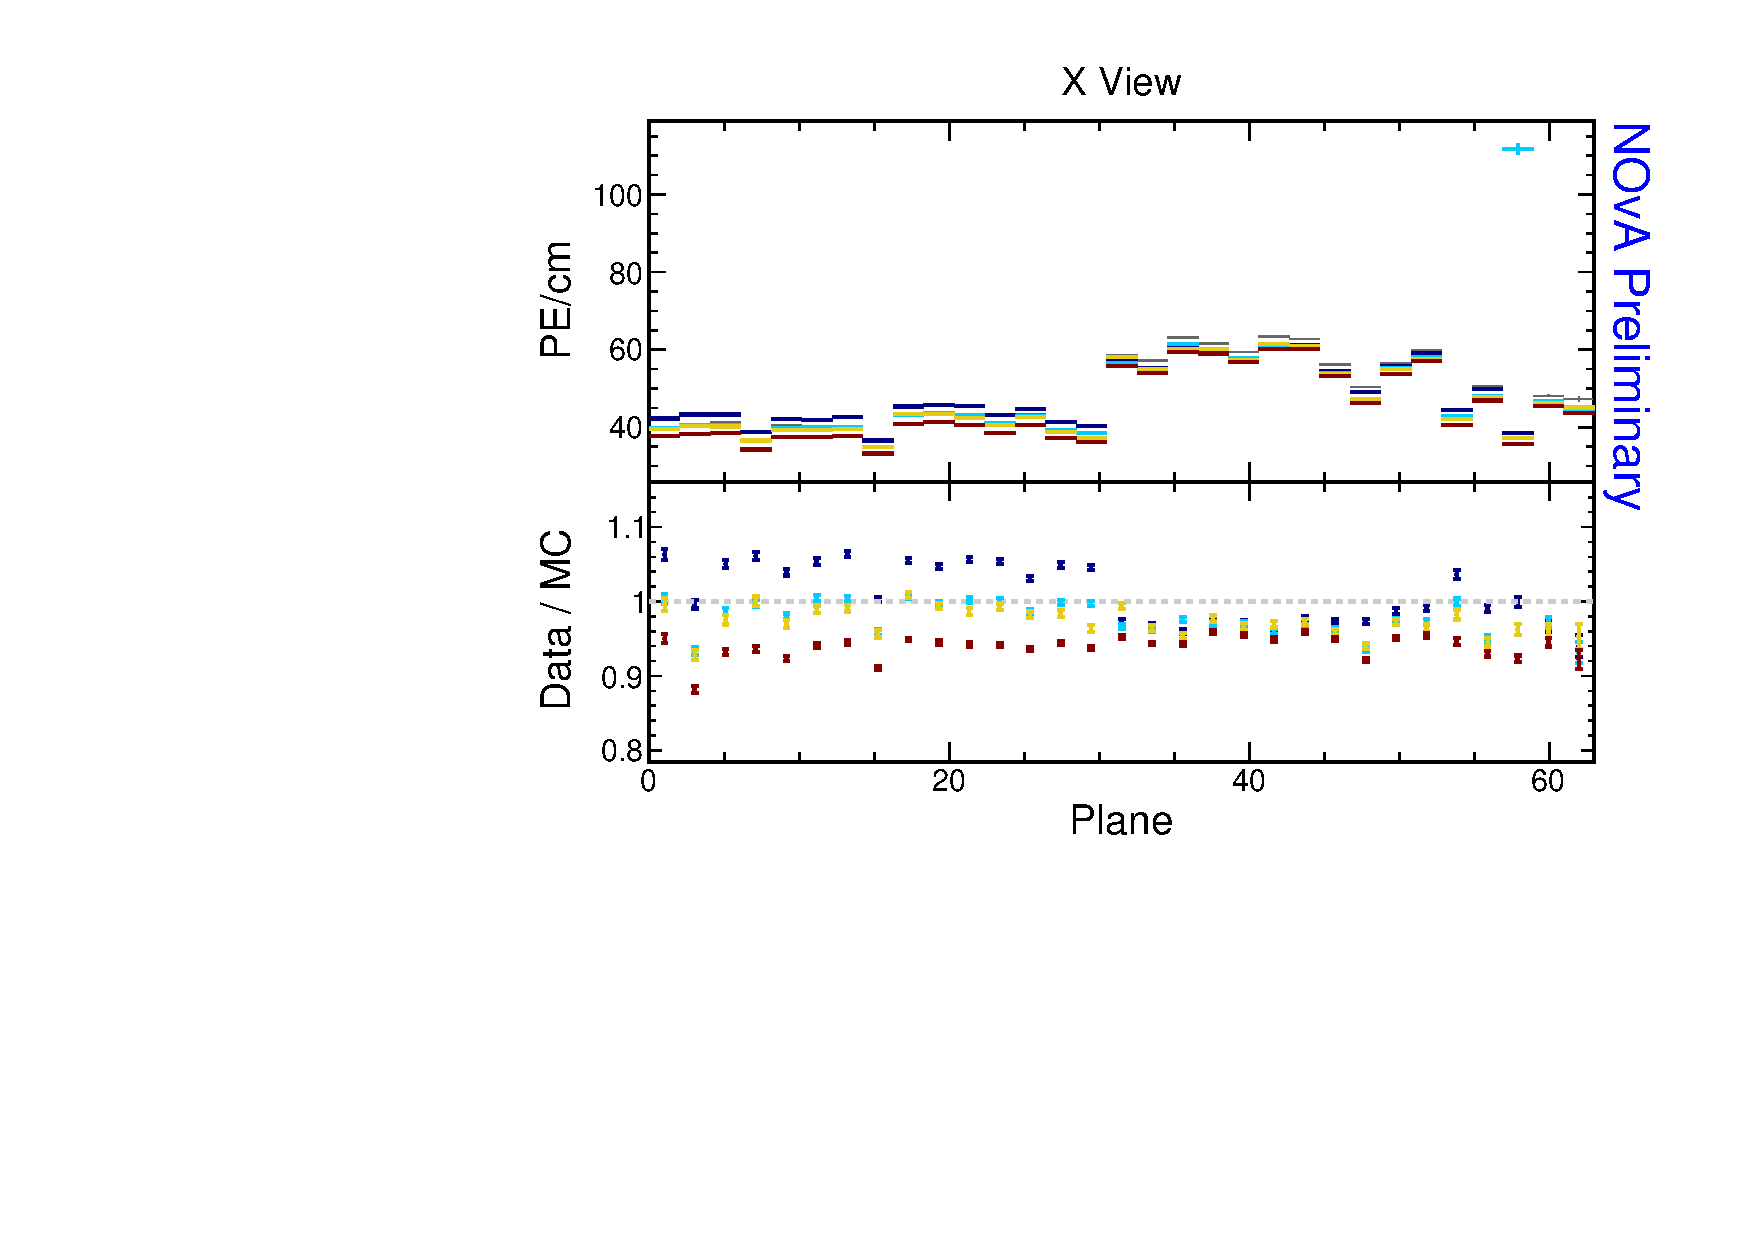
\includegraphics[width=\linewidth]{Plots/Calibana/pecm_plane_x.pdf}
  \end{subfigure}
  \begin{subfigure}{0.495\textwidth}
    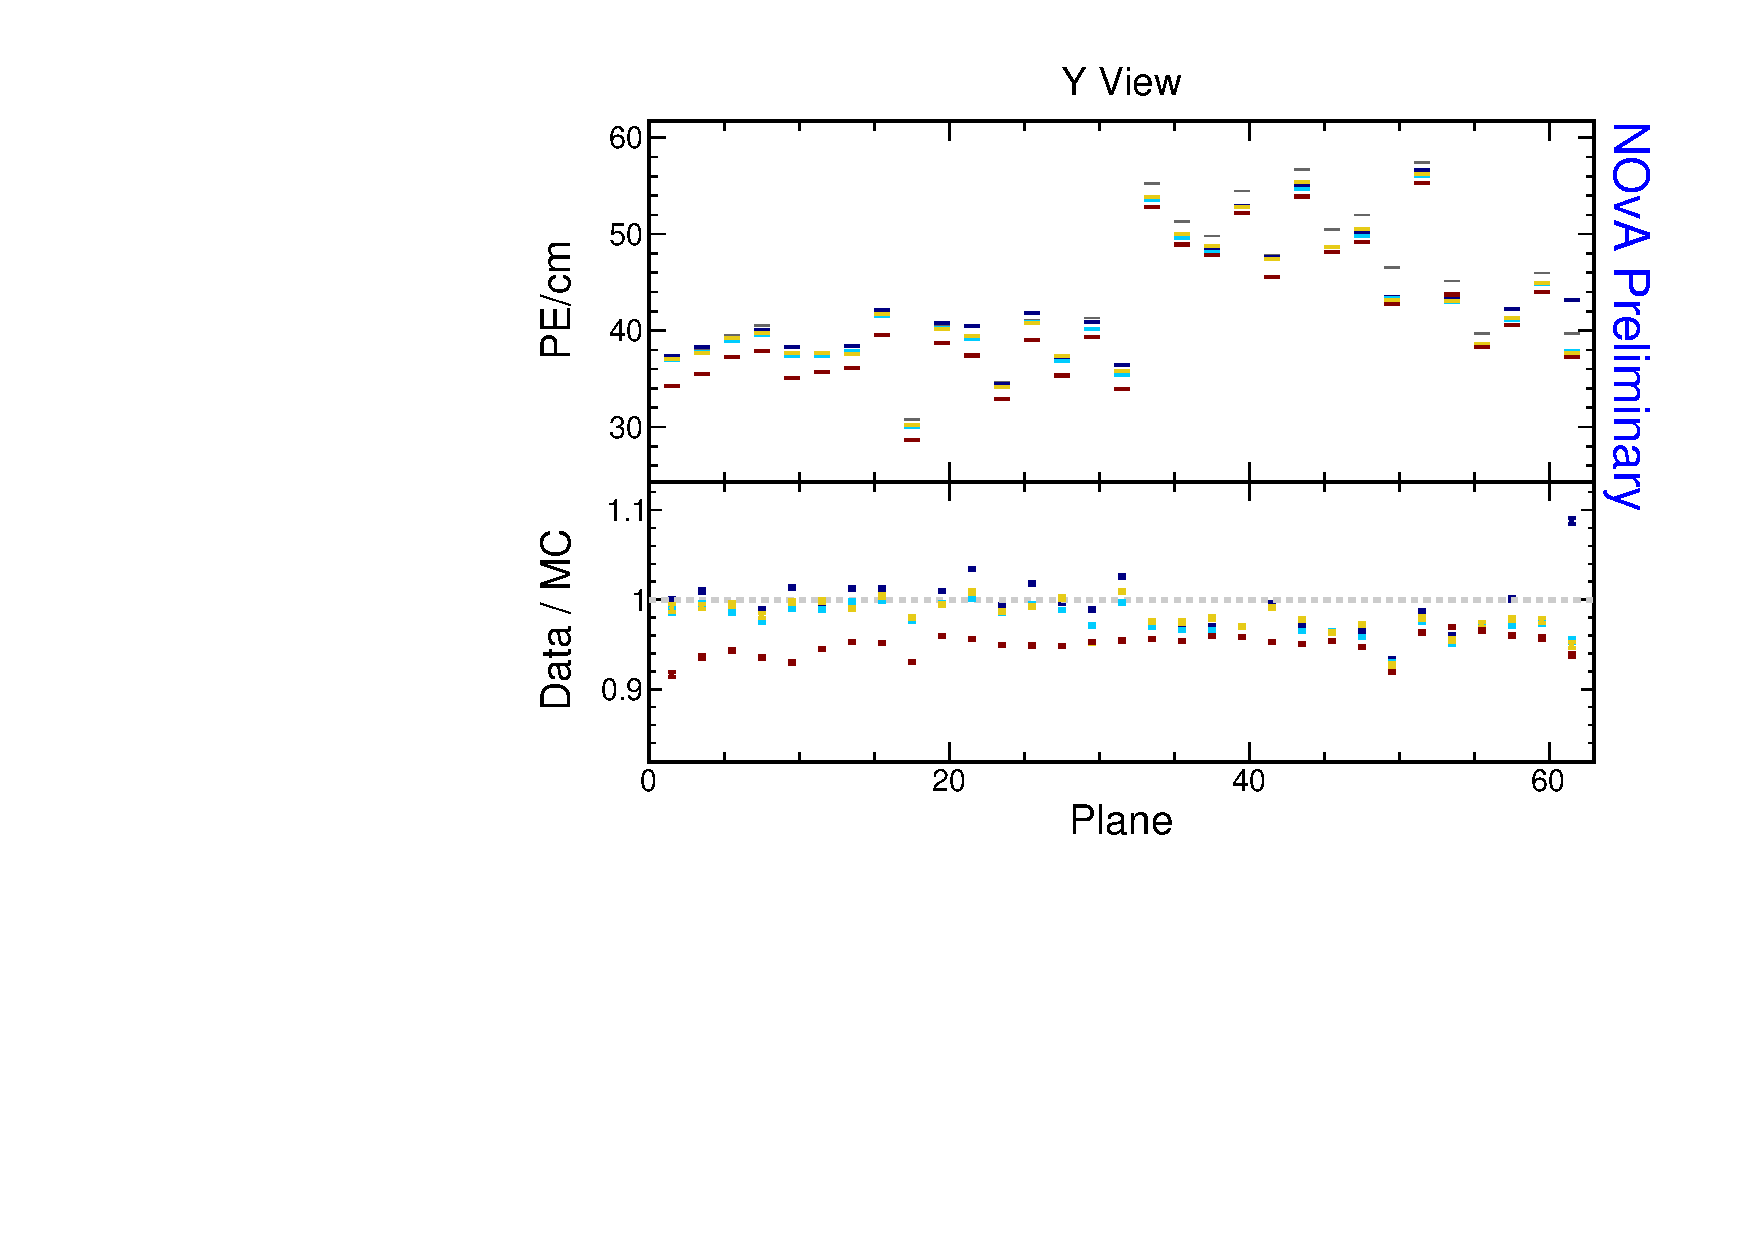
\includegraphics[width=\linewidth]{Plots/Calibana/pecm_plane_y.pdf}
  \end{subfigure}
  \begin{subfigure}{0.495\textwidth}
    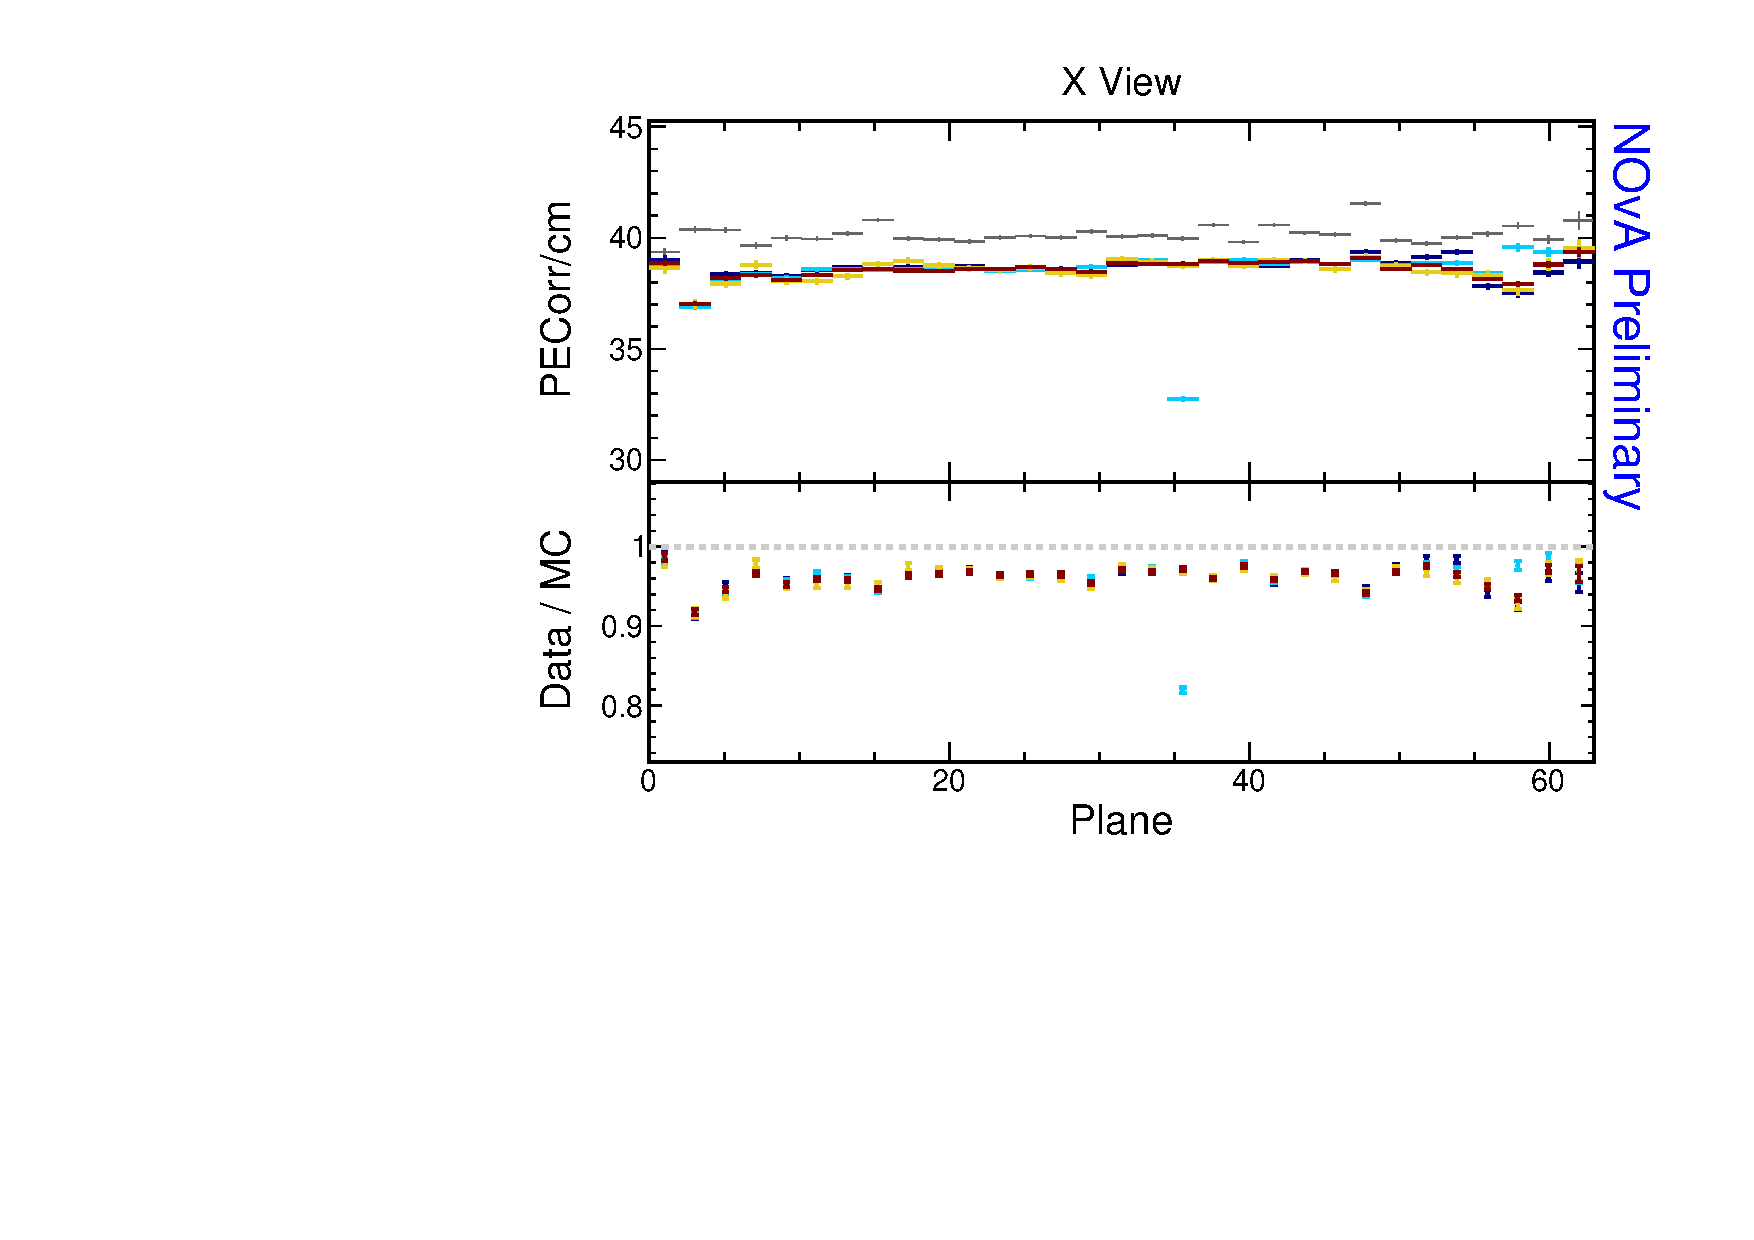
\includegraphics[width=\linewidth]{Plots/Calibana/pecorrcm_plane_x.pdf}
  \end{subfigure}
  \begin{subfigure}{0.495\textwidth}
    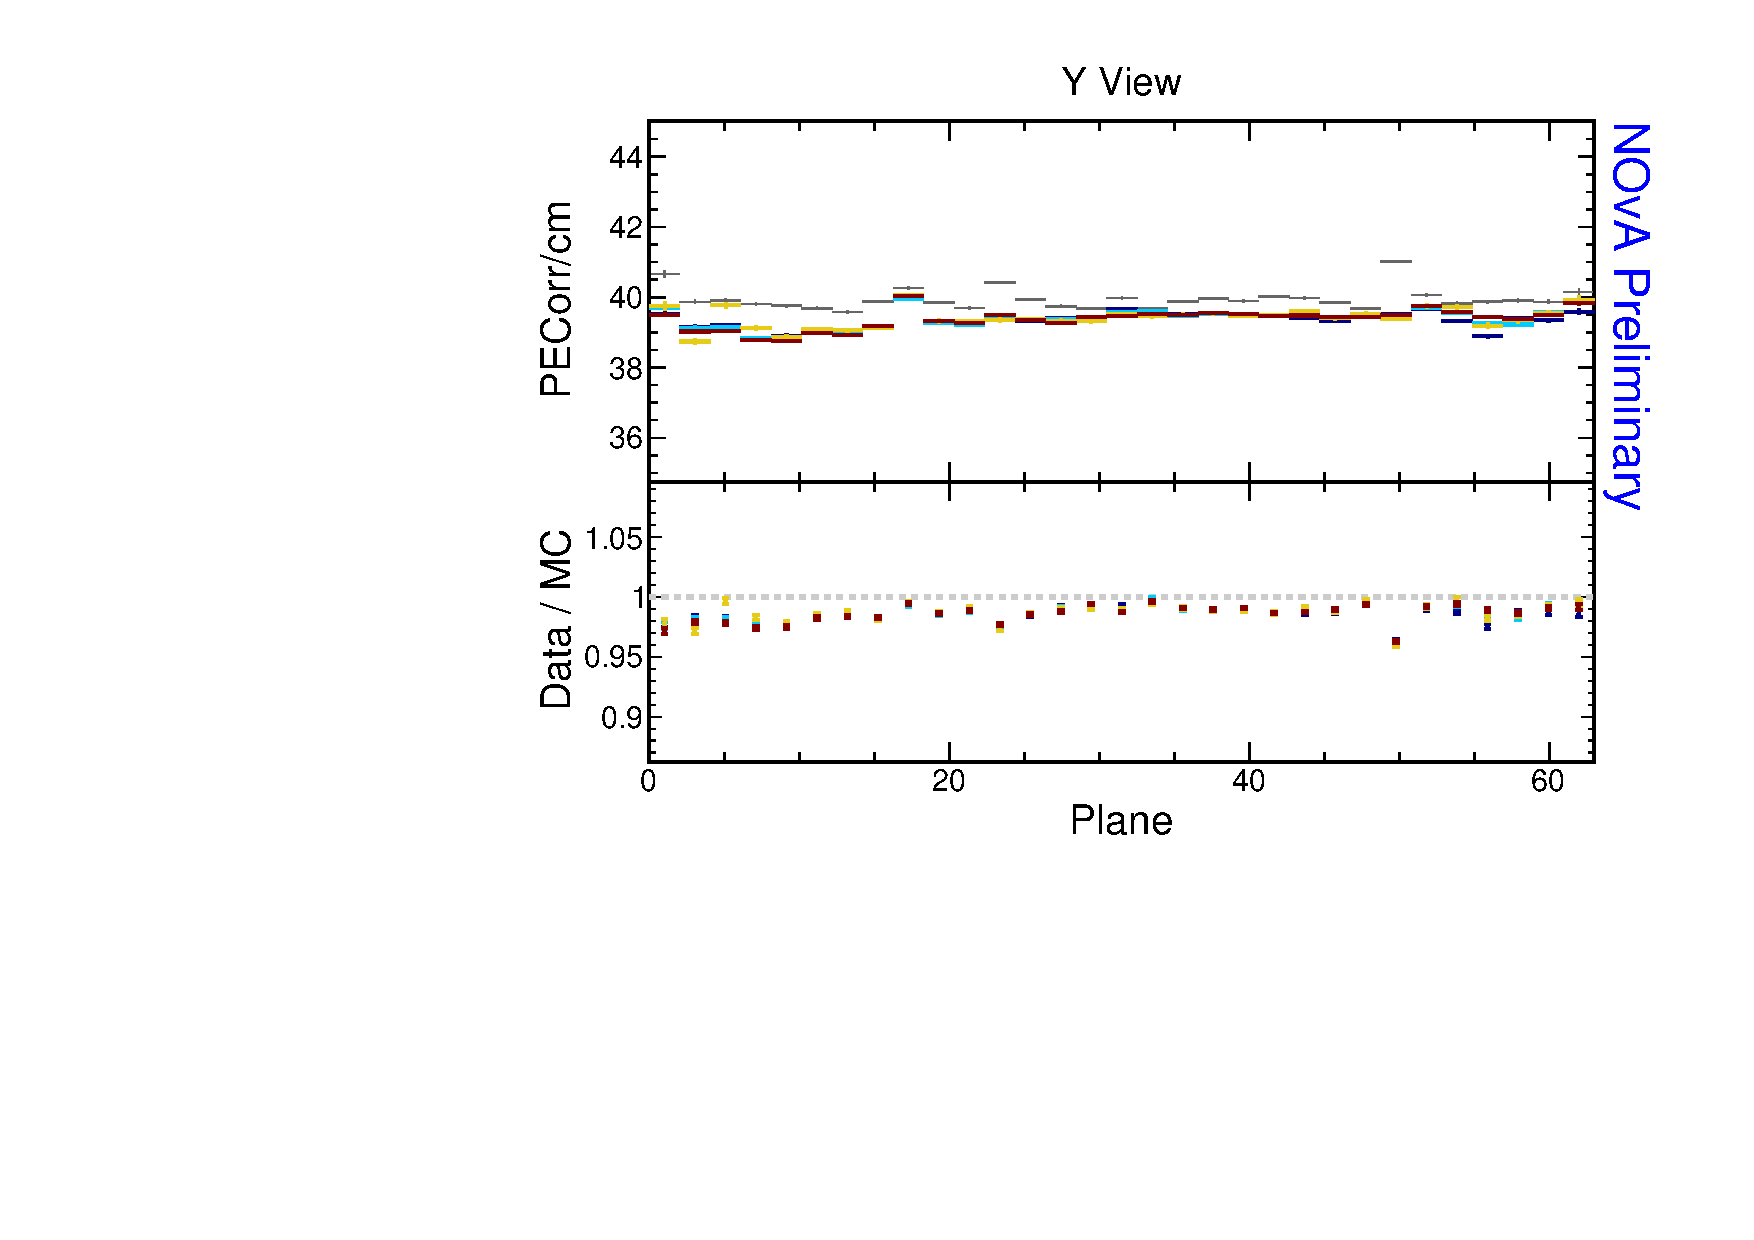
\includegraphics[width=\linewidth]{Plots/Calibana/pecorrcm_plane_y.pdf}
  \end{subfigure}
    \begin{subfigure}{0.495\textwidth}
    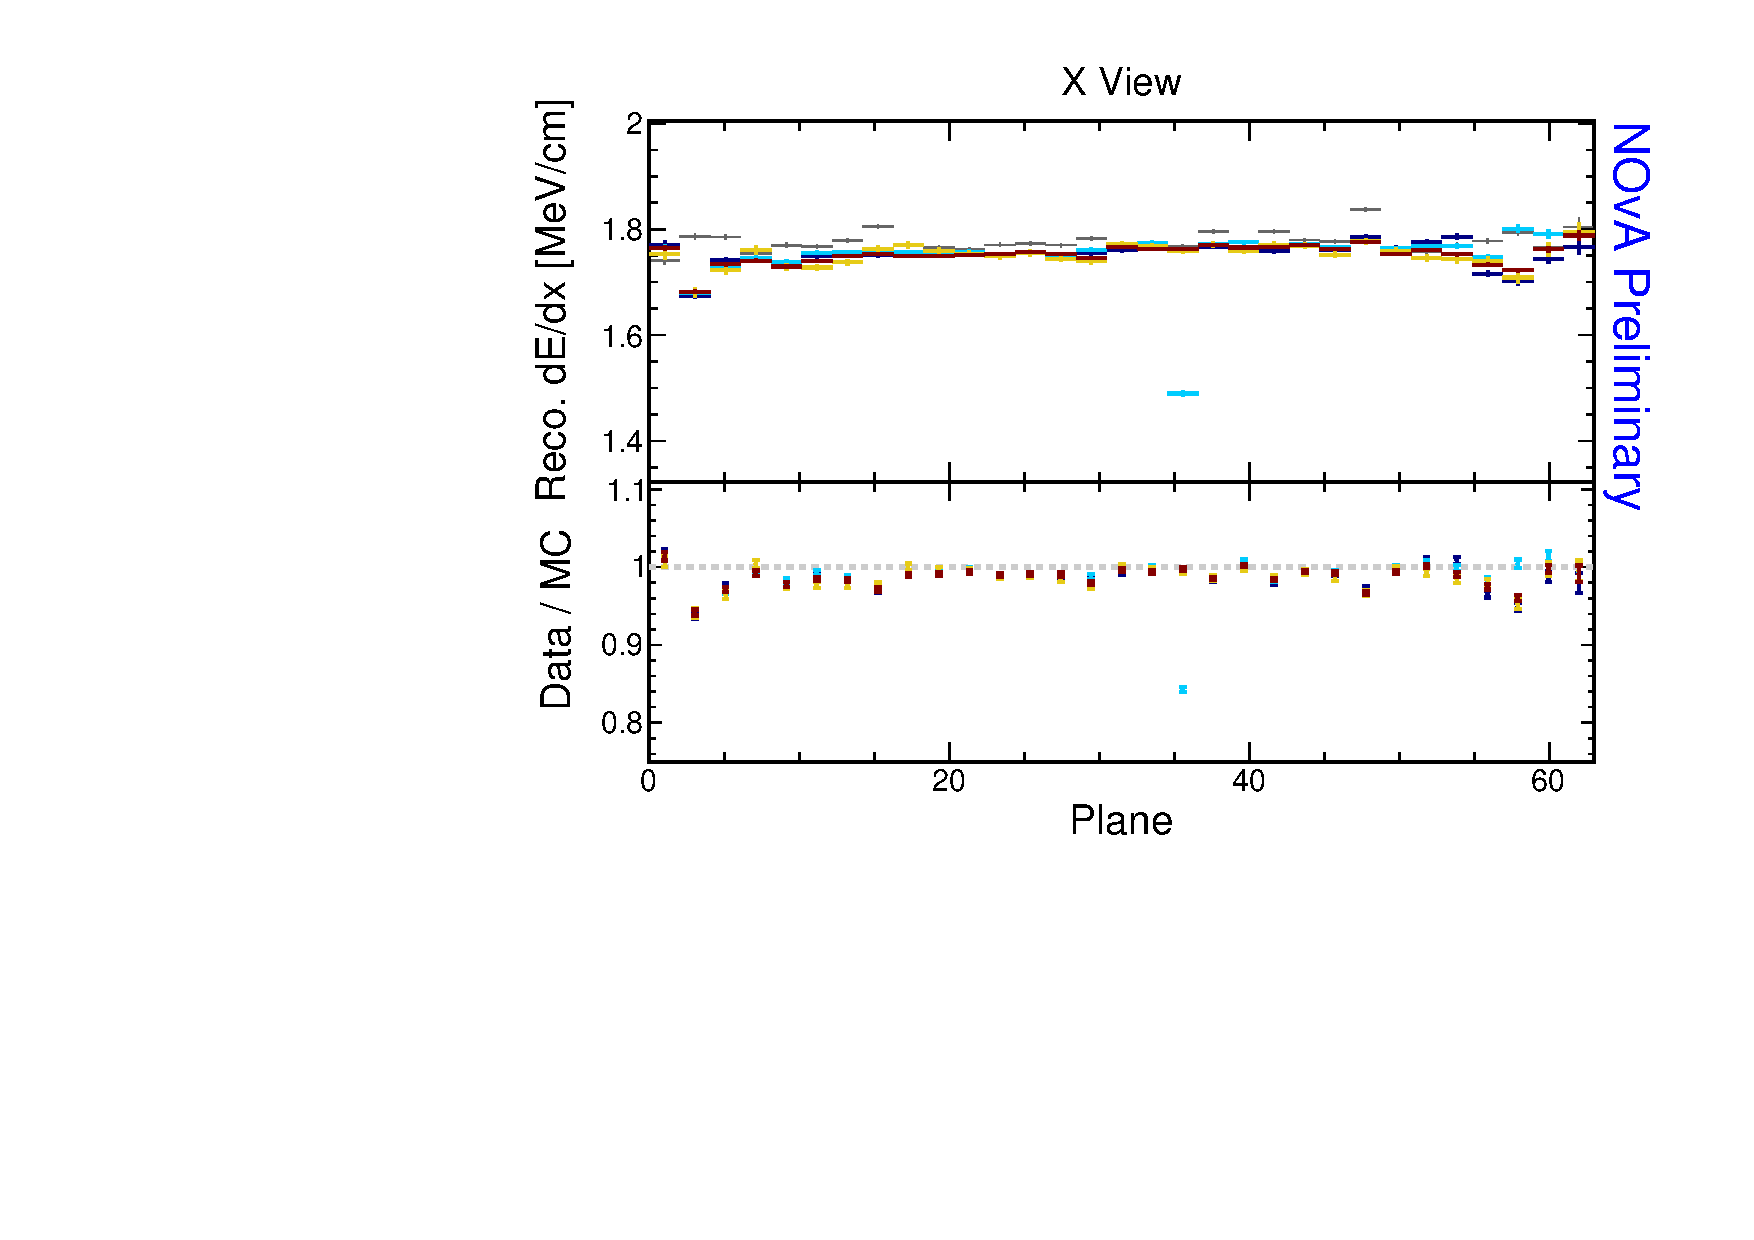
\includegraphics[width=\linewidth]{Plots/Calibana/recomevcm_plane_x.pdf}
  \end{subfigure}
  \begin{subfigure}{0.495\textwidth}
    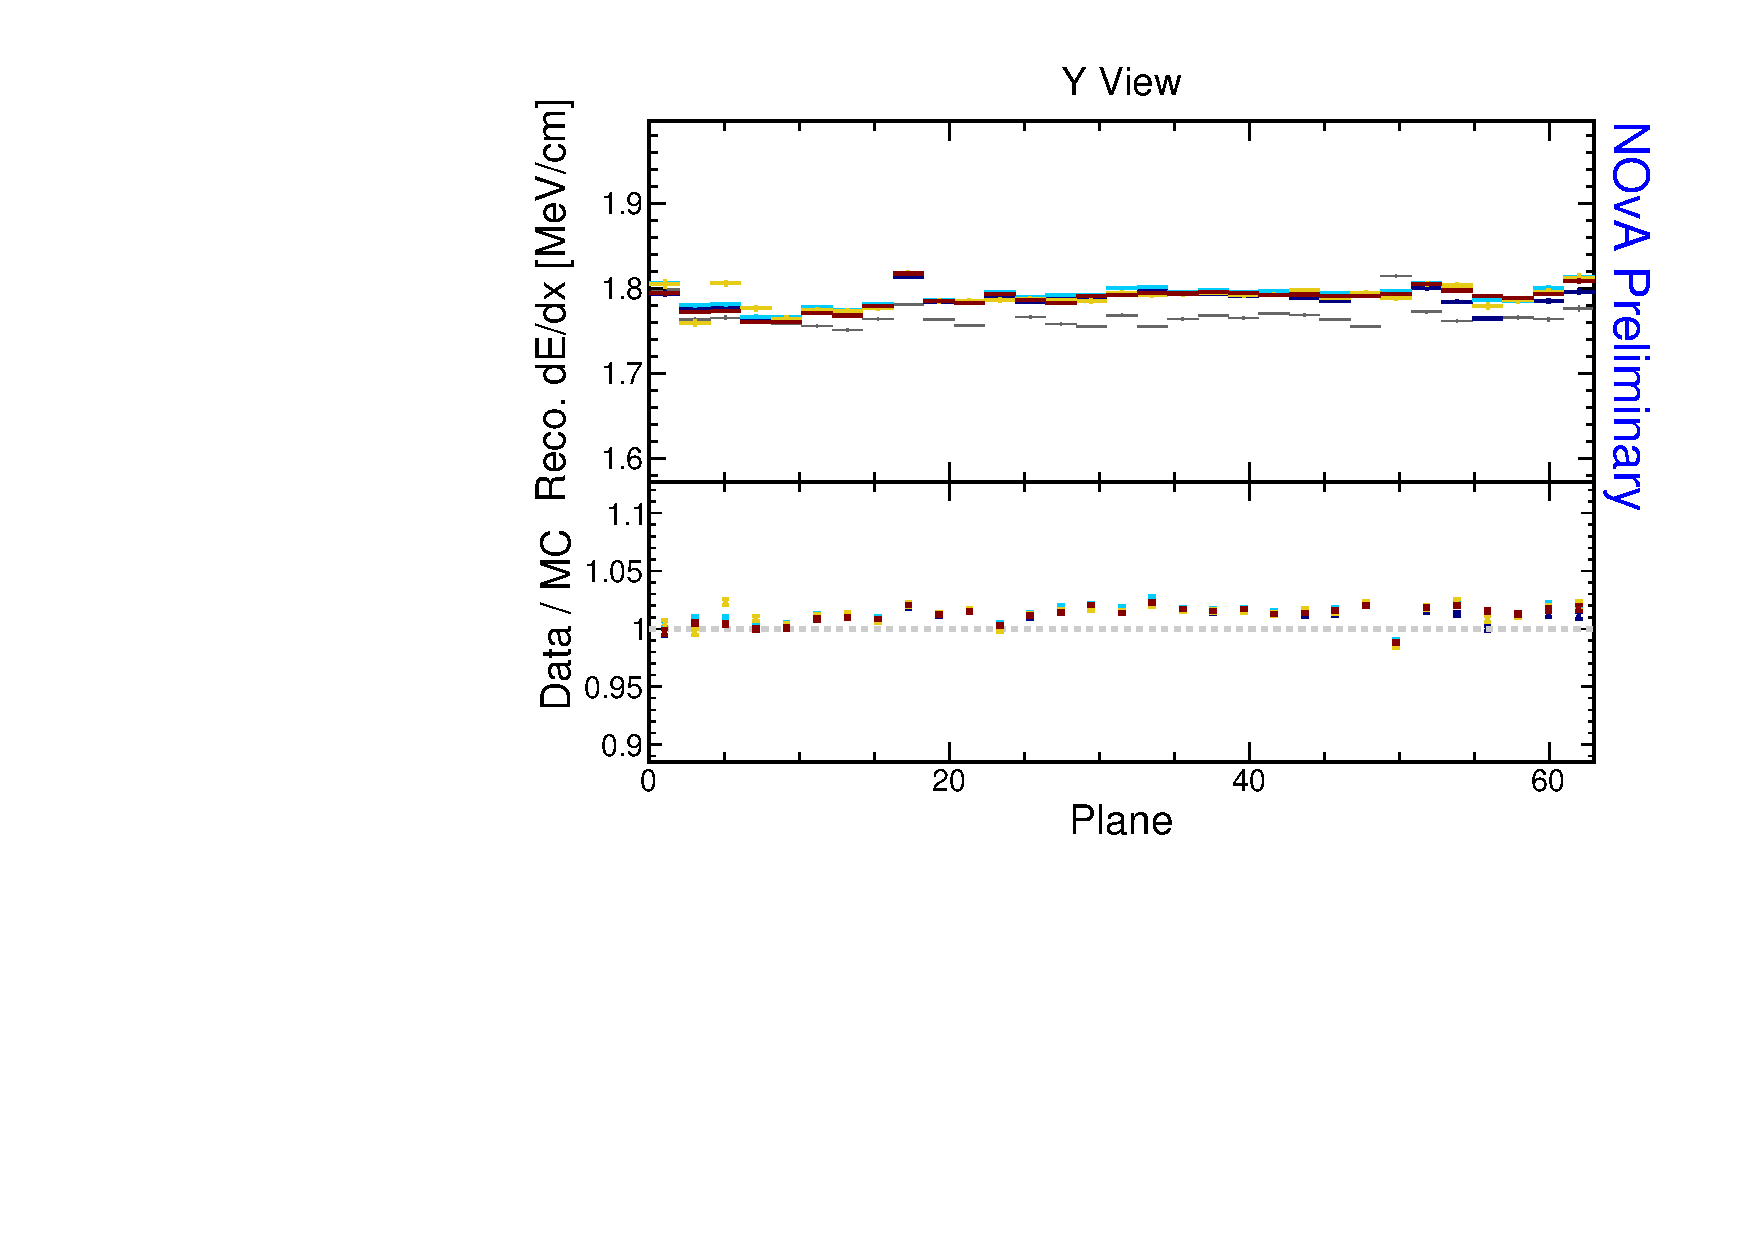
\includegraphics[width=\linewidth]{Plots/Calibana/recomevcm_plane_y.pdf}
  \end{subfigure}
  \caption[Energy deposition of stopping muons across planes]{Distributions of stopping muons within a 1-2 m track window from the end of their tracks across the detector planes for simulation (gray) and all the Test Beam data samples. The top row shows the energy deposition before any correction, middle row after relative calibration corrections and bottom row after full calibration corrections. The left column shows the X view (vertical planes) and right column the Y view (horizontal planes).}
  %\label{fig:AbsCalibPlane1}
\end{figure}

\begin{figure}[!ht]
  \begin{subfigure}{\textwidth}
  \centering
    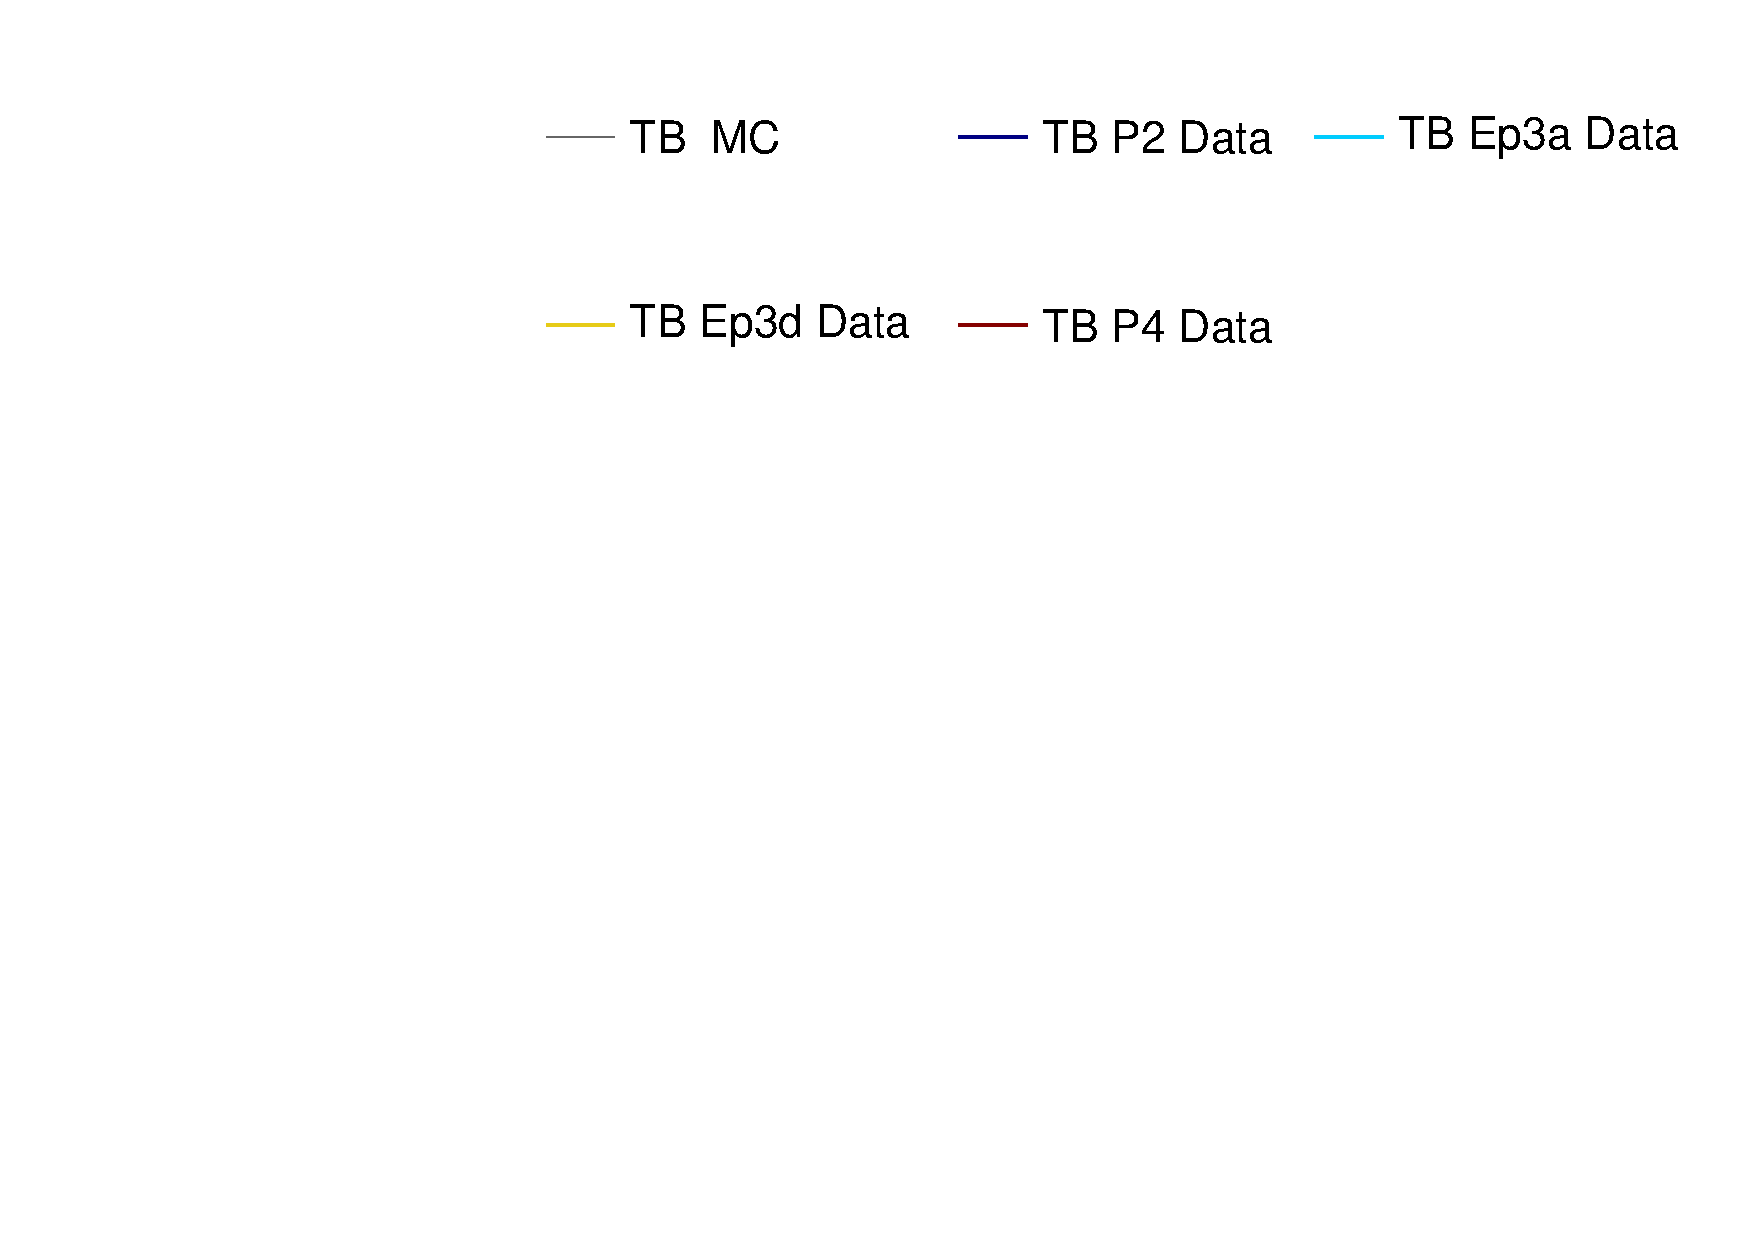
\includegraphics[height=0.2\linewidth]{Plots/Calibana/legend.pdf}
  \end{subfigure}
  \vspace*{2mm}

  \begin{subfigure}{0.495\textwidth}
    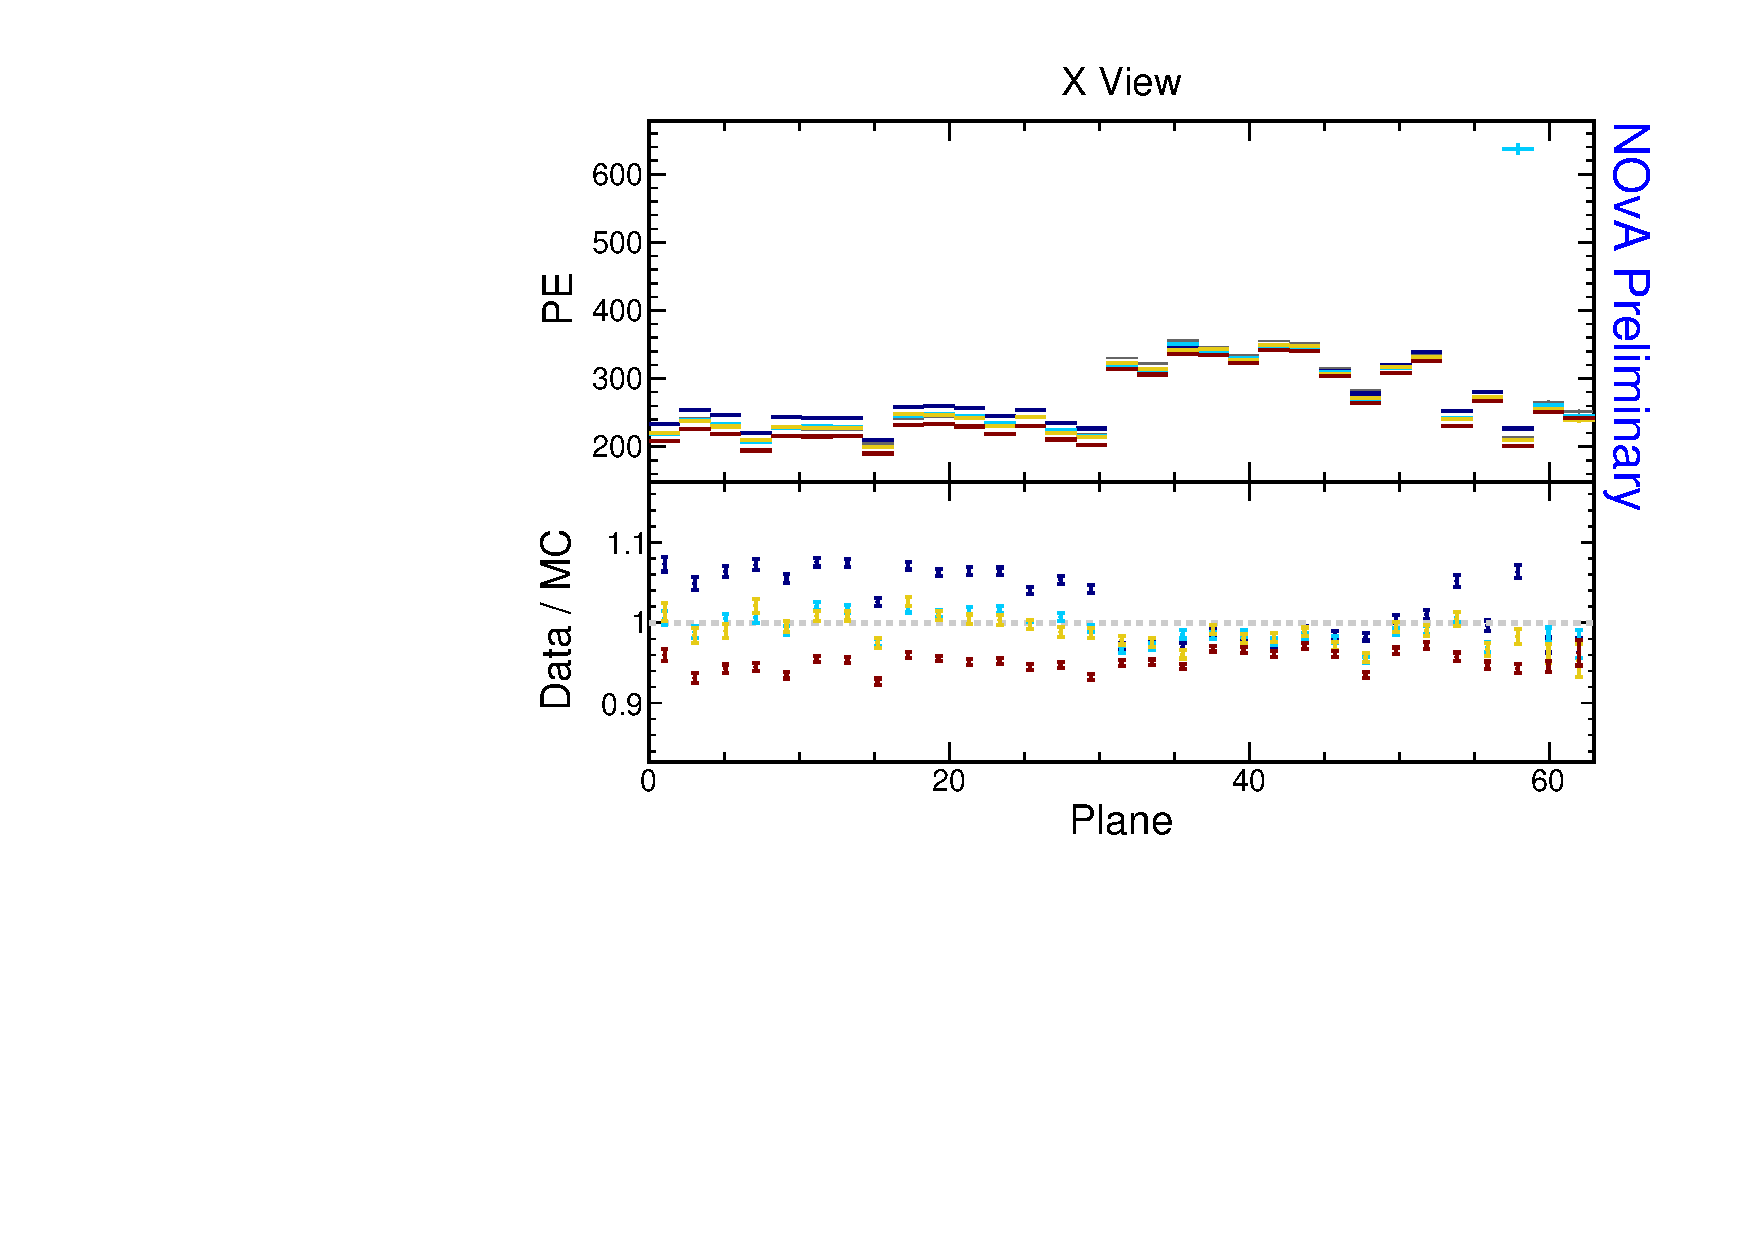
\includegraphics[width=\linewidth]{Plots/Calibana/pe_plane_x.pdf}
  \end{subfigure}
  \begin{subfigure}{0.495\textwidth}
    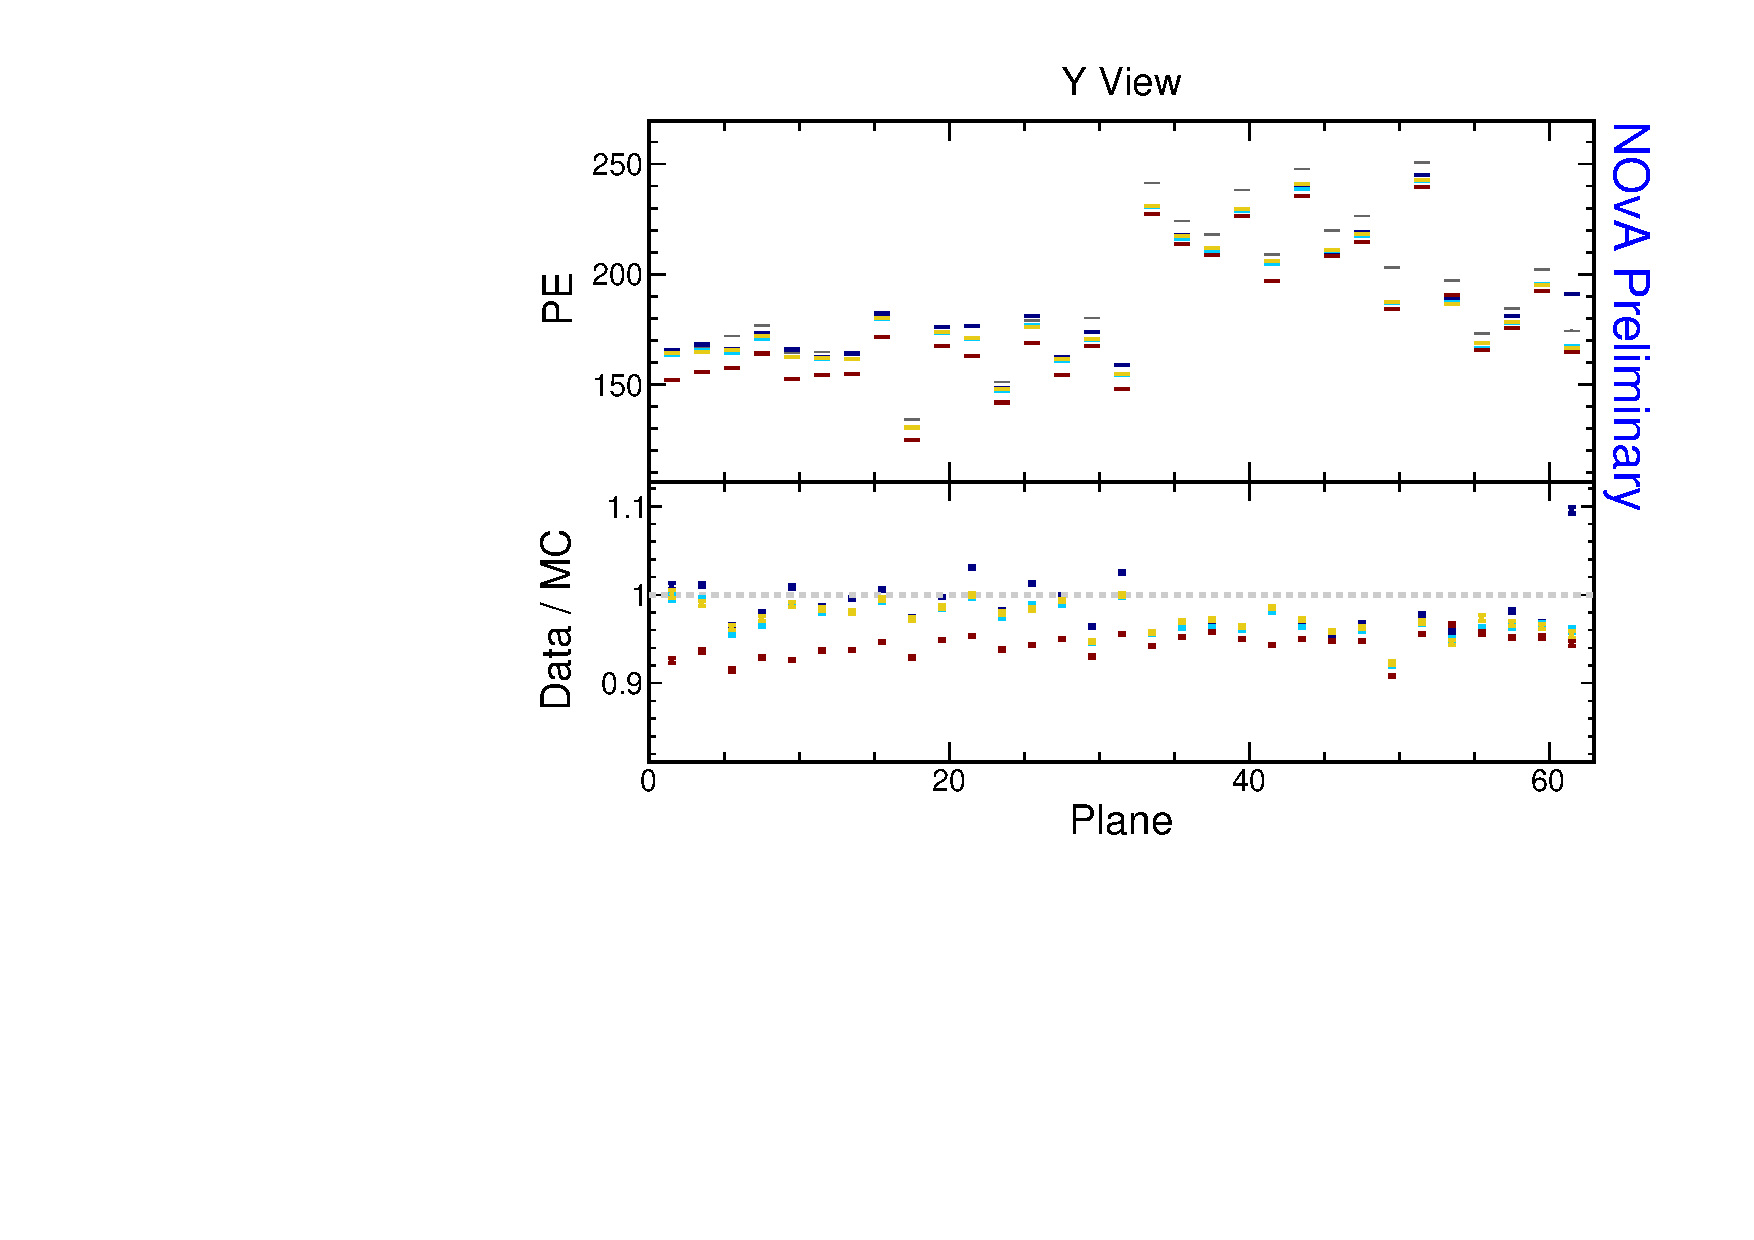
\includegraphics[width=\linewidth]{Plots/Calibana/pe_plane_y.pdf}
  \end{subfigure}
  \begin{subfigure}{0.495\textwidth}
    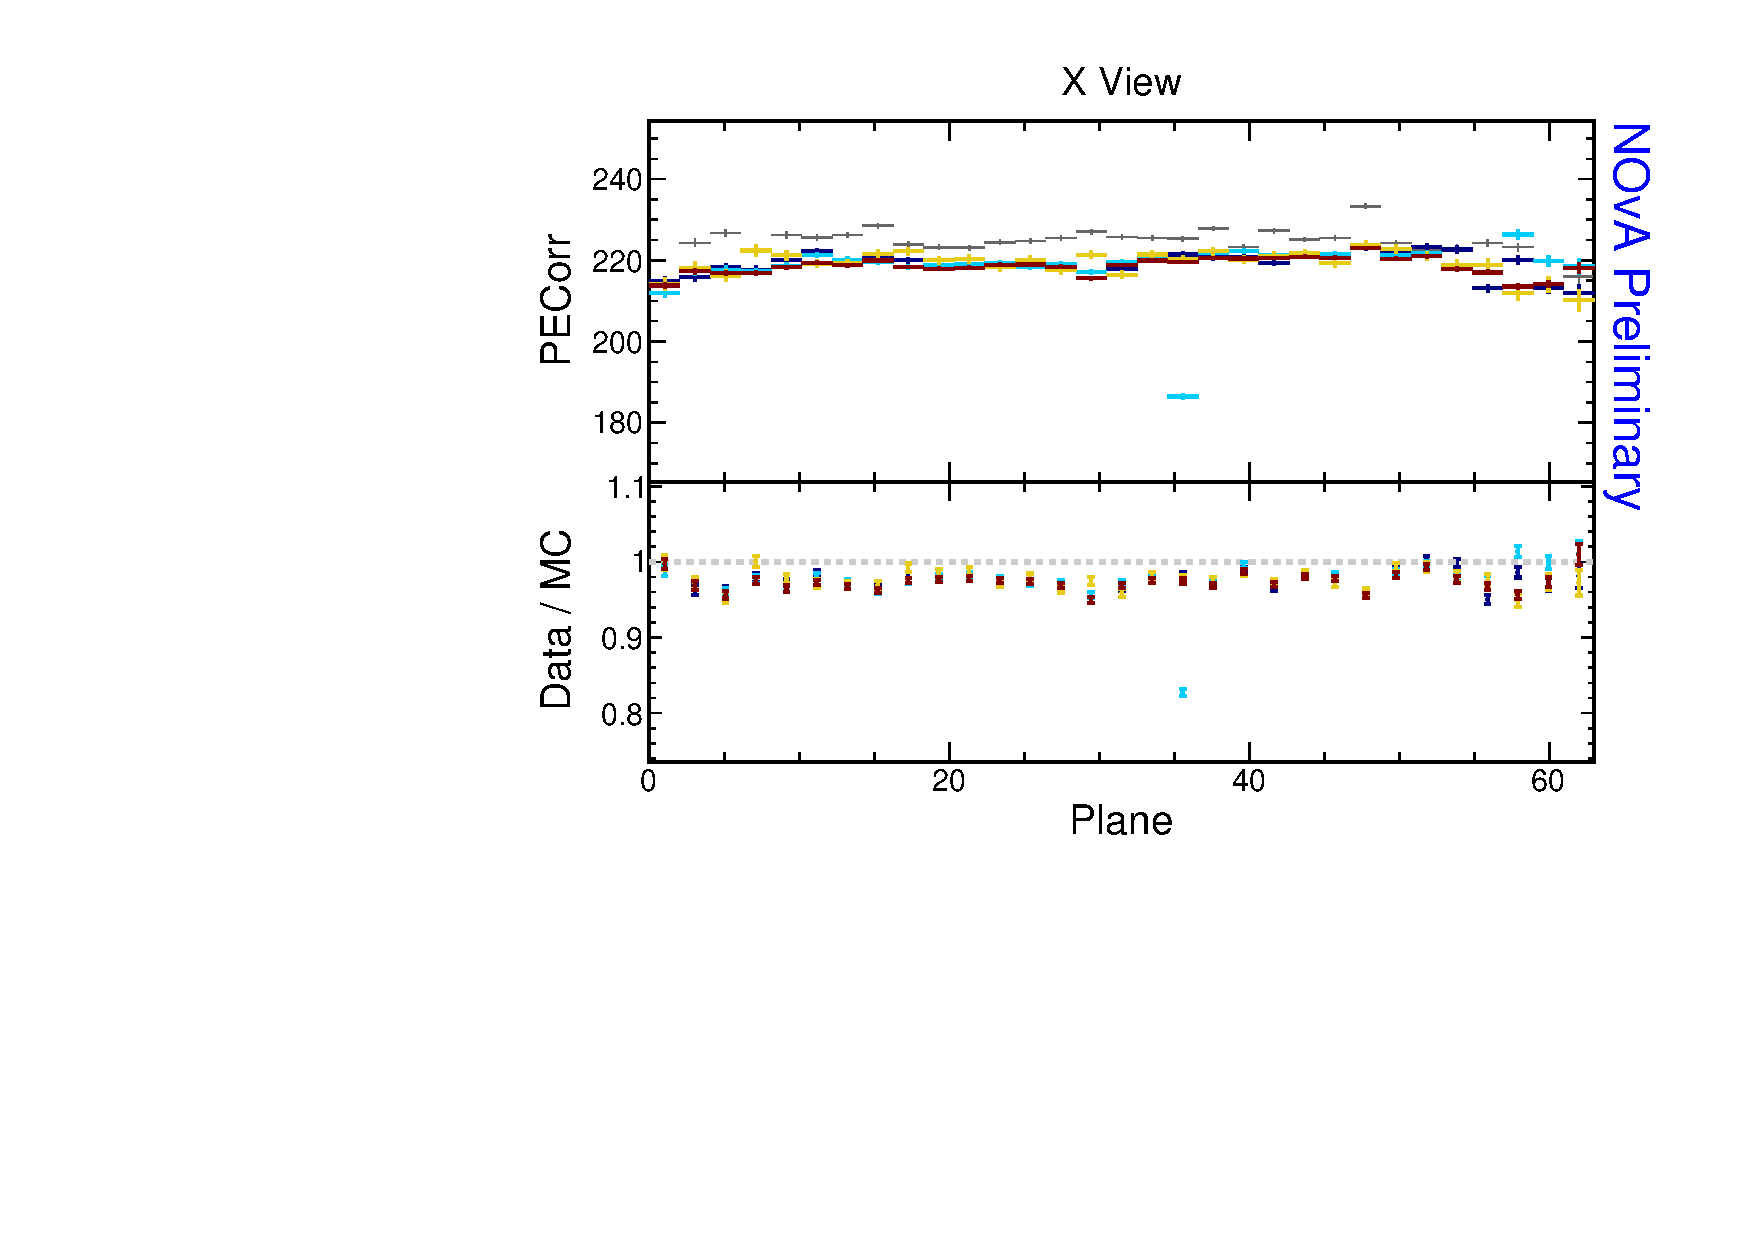
\includegraphics[width=\linewidth]{Plots/Calibana/pecorr_plane_x.pdf}
  \end{subfigure}
  \begin{subfigure}{0.495\textwidth}
    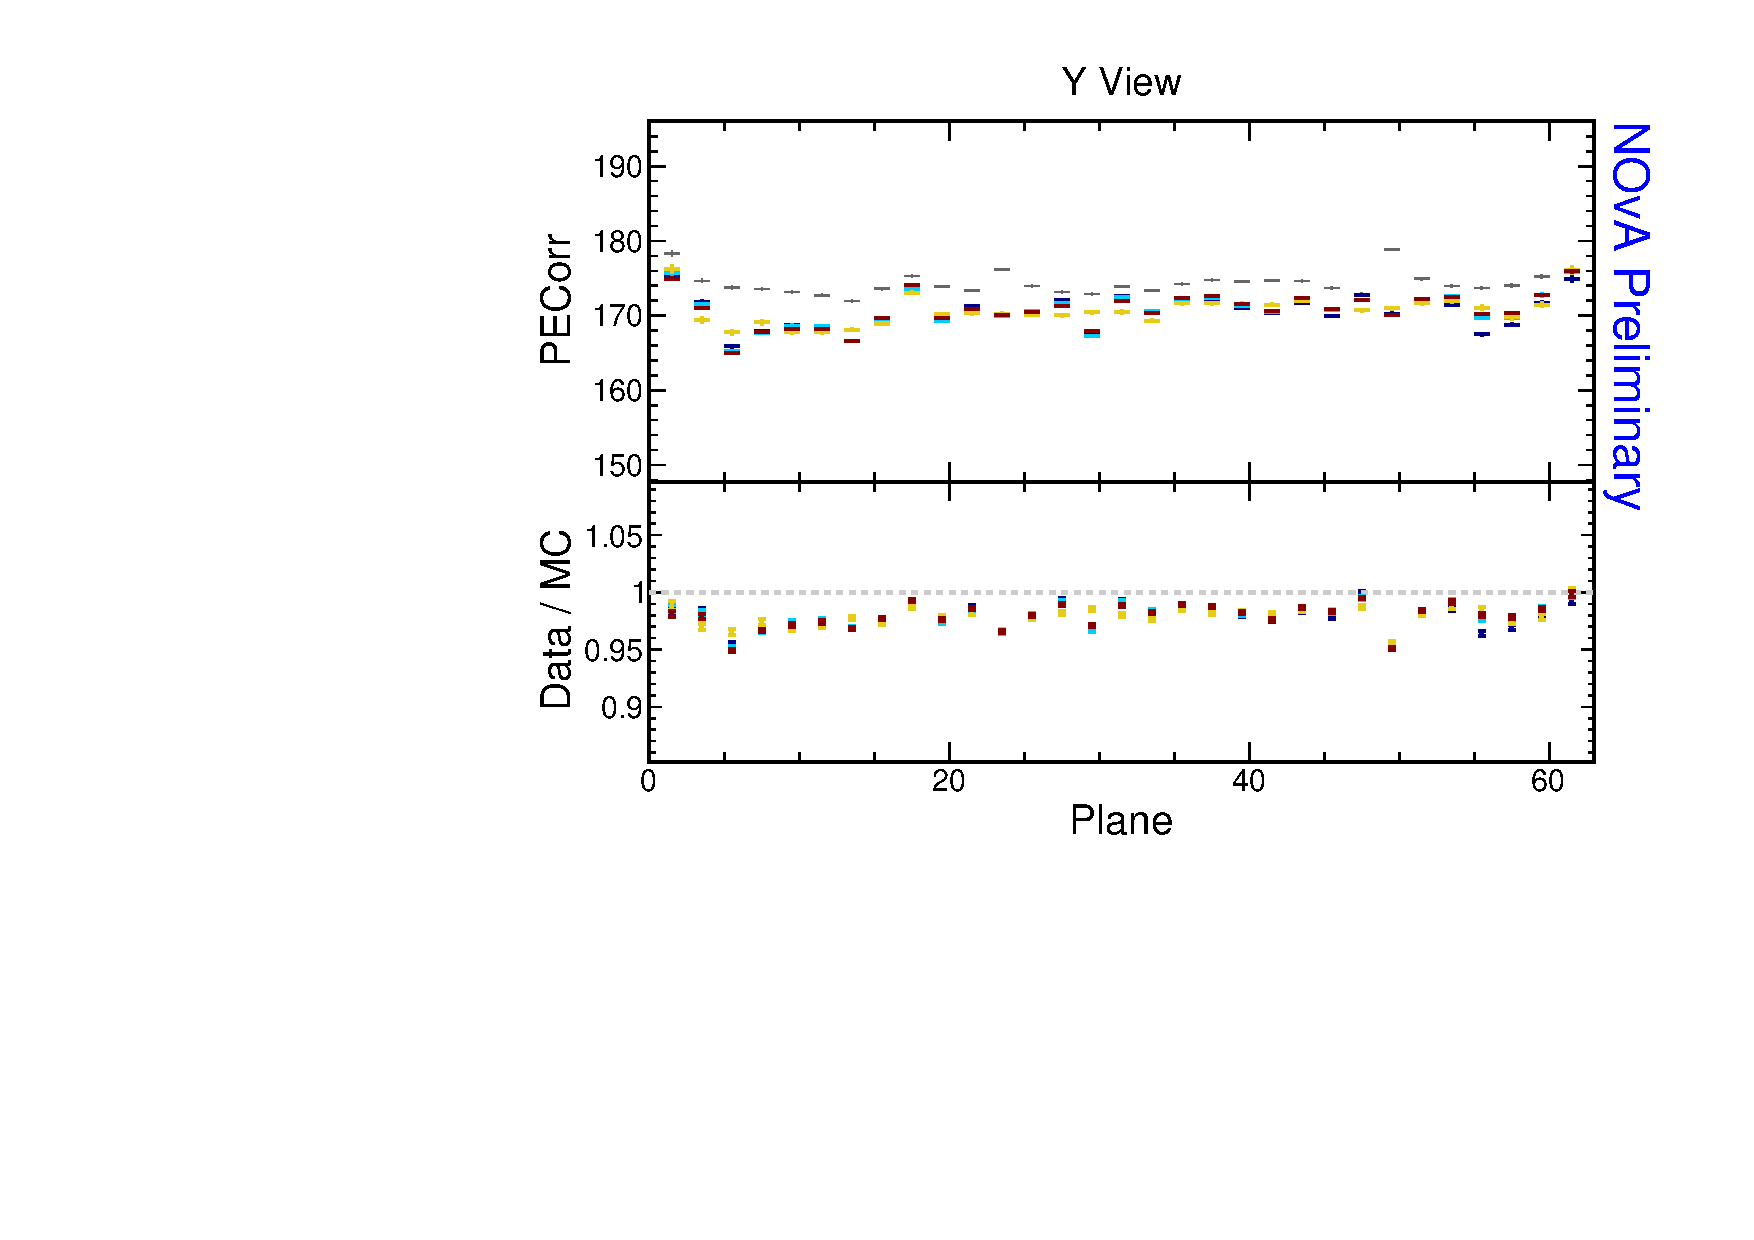
\includegraphics[width=\linewidth]{Plots/Calibana/pecorr_plane_y.pdf}
  \end{subfigure}
  \begin{subfigure}{0.495\textwidth}
    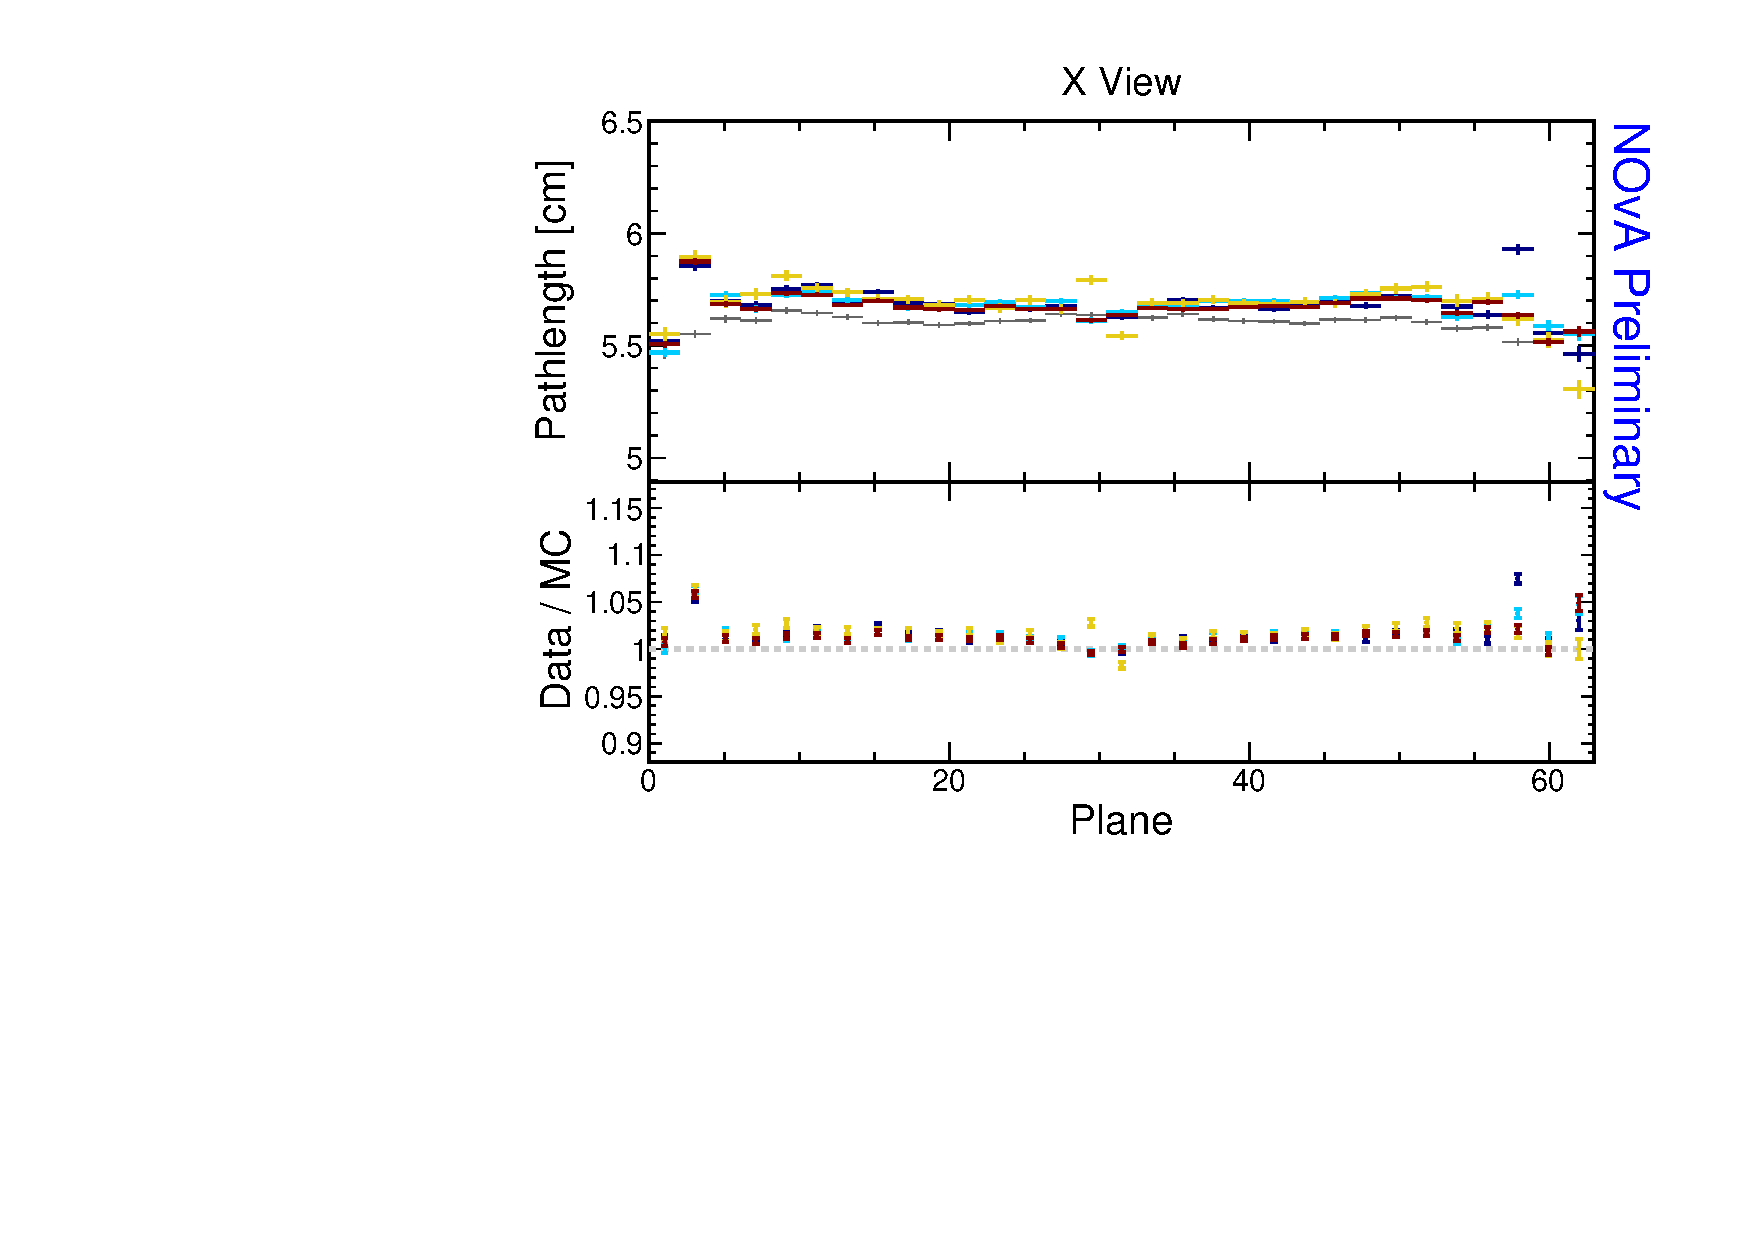
\includegraphics[width=\linewidth]{Plots/Calibana/cm_plane_x.pdf}
  \end{subfigure}
  \begin{subfigure}{0.495\textwidth}
    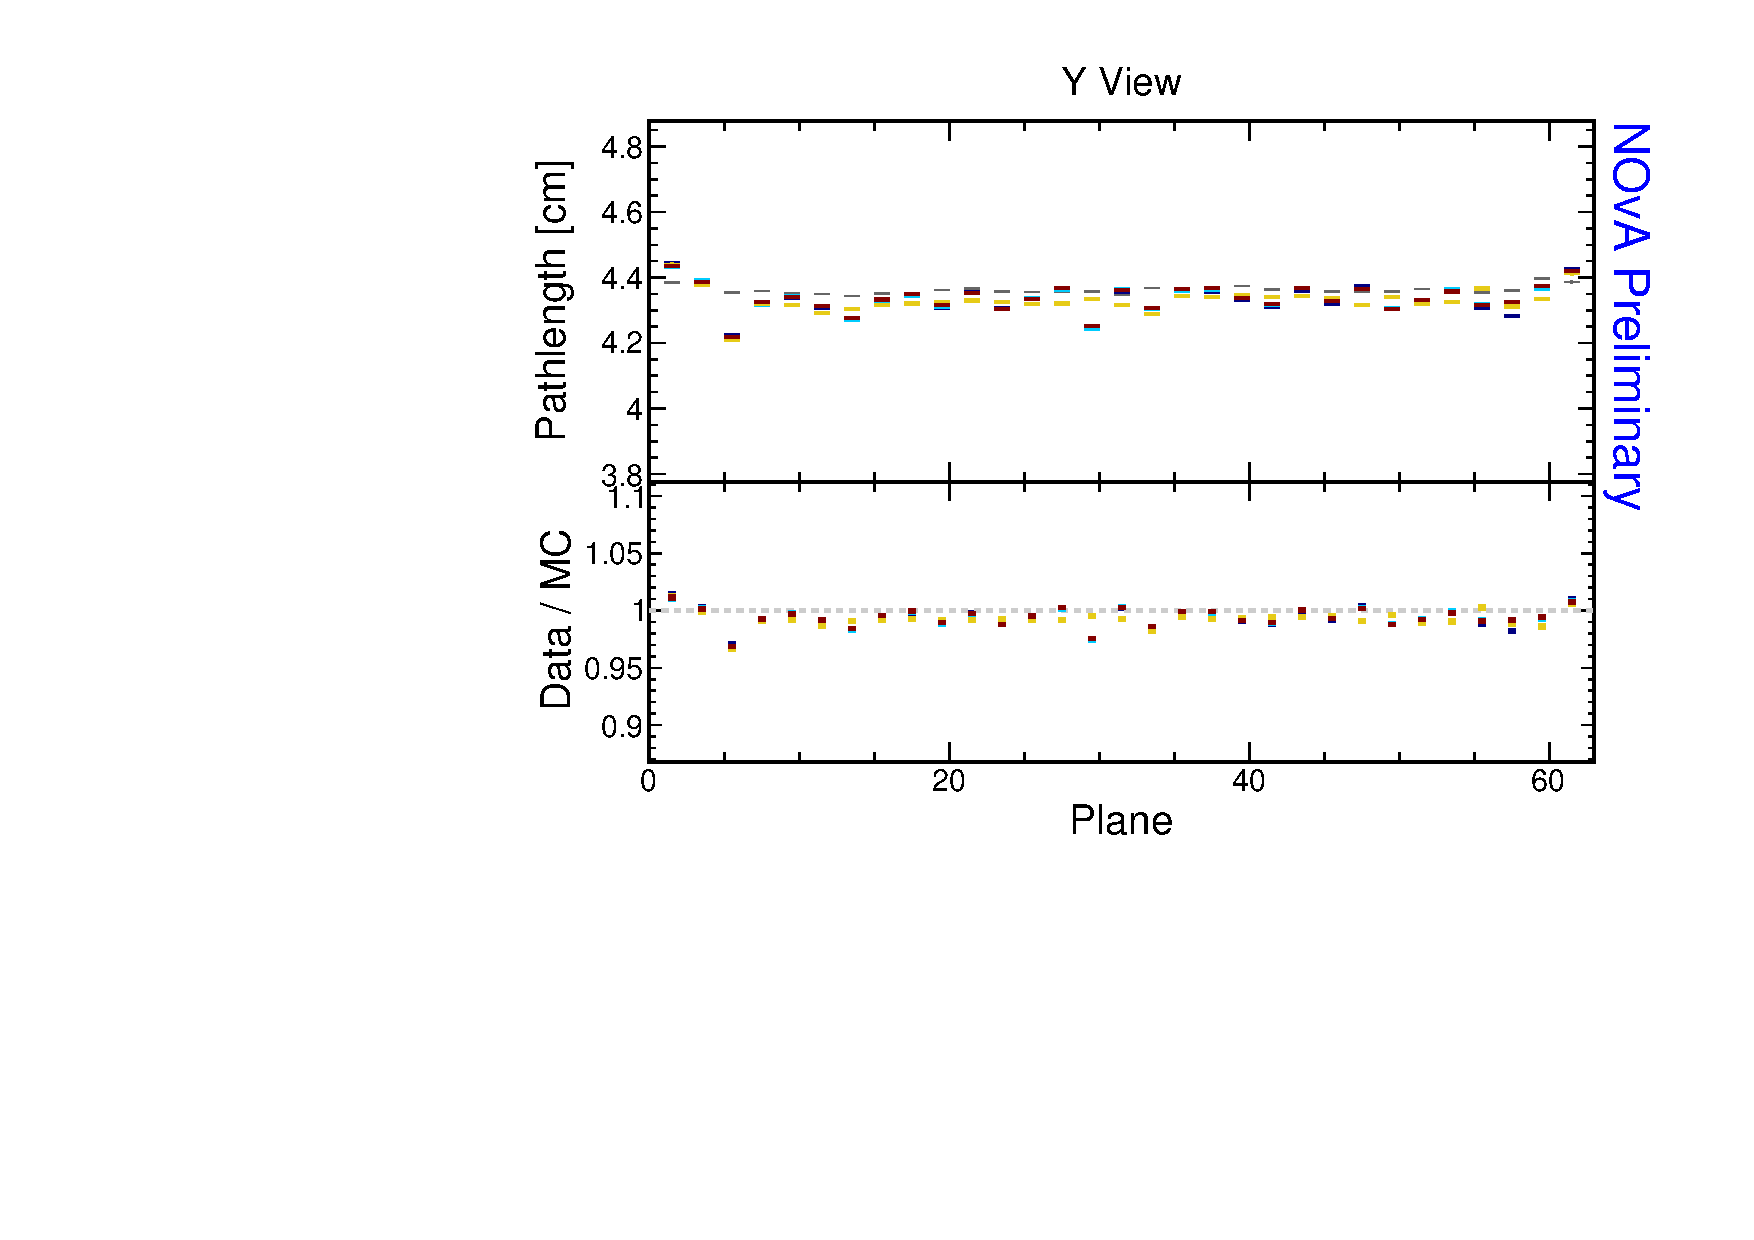
\includegraphics[width=\linewidth]{Plots/Calibana/cm_plane_y.pdf}
  \end{subfigure}
  \caption[Calibration variables of stopping muons along planes]{Distributions of stopping muons within a 1-2 m track window from the end of their tracks across the detector planes for simulation (gray) and all the Test Beam data samples. The top row shows the number of recorded photo electrons before any corrections, middle row shows the same after relative calibration corrections and bottom row shows the path length through the cell. The left column shows the X view (vertical planes) and right column the Y view (horizontal planes).}
  %\label{fig:AbsCalibPlane2}
\end{figure}

%\subsection{Drift in TB data}

\begin{figure}[!ht]
  \begin{subfigure}{\textwidth}
    \centering
    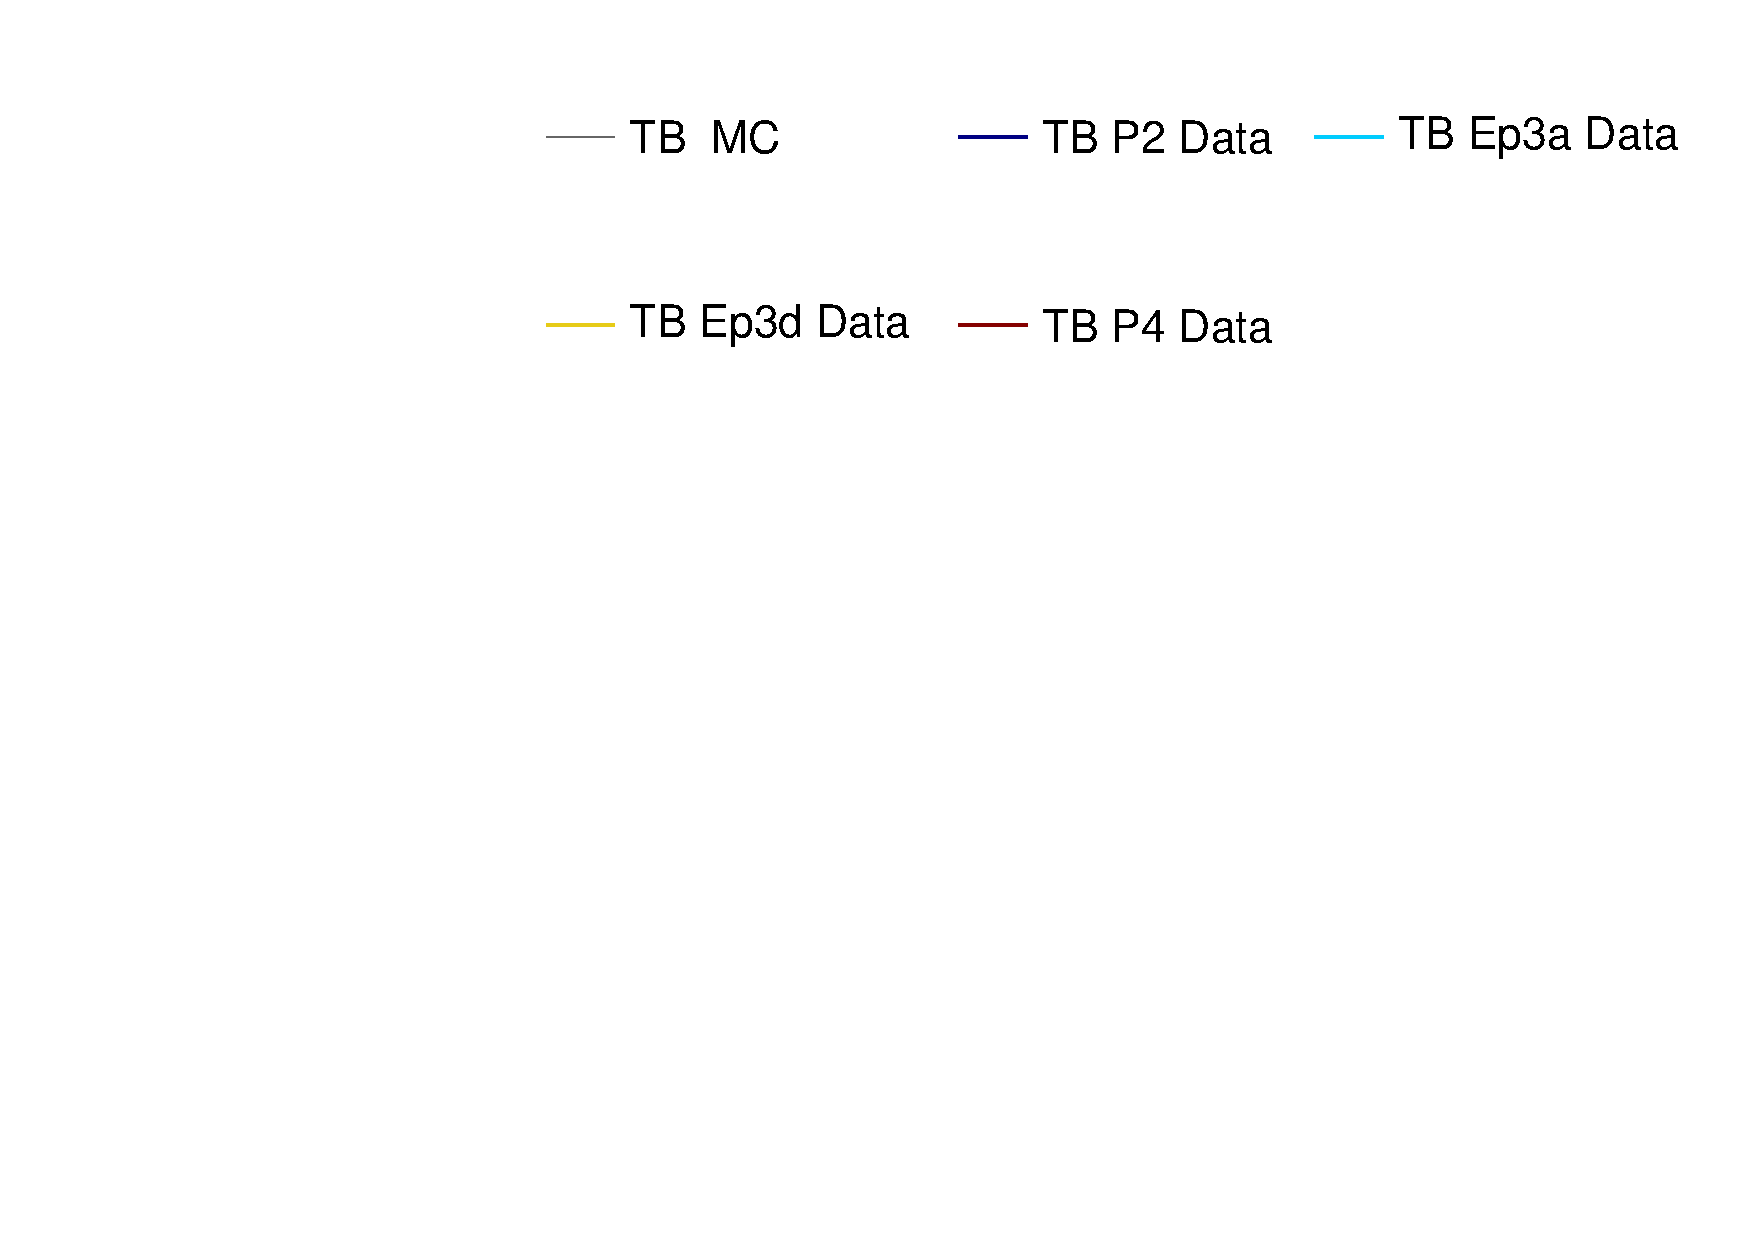
\includegraphics[height=0.2\linewidth]{Plots/Calibana/legend.pdf}
  \end{subfigure}
  \vspace*{2mm}
  
  \begin{subfigure}{0.495\textwidth}
    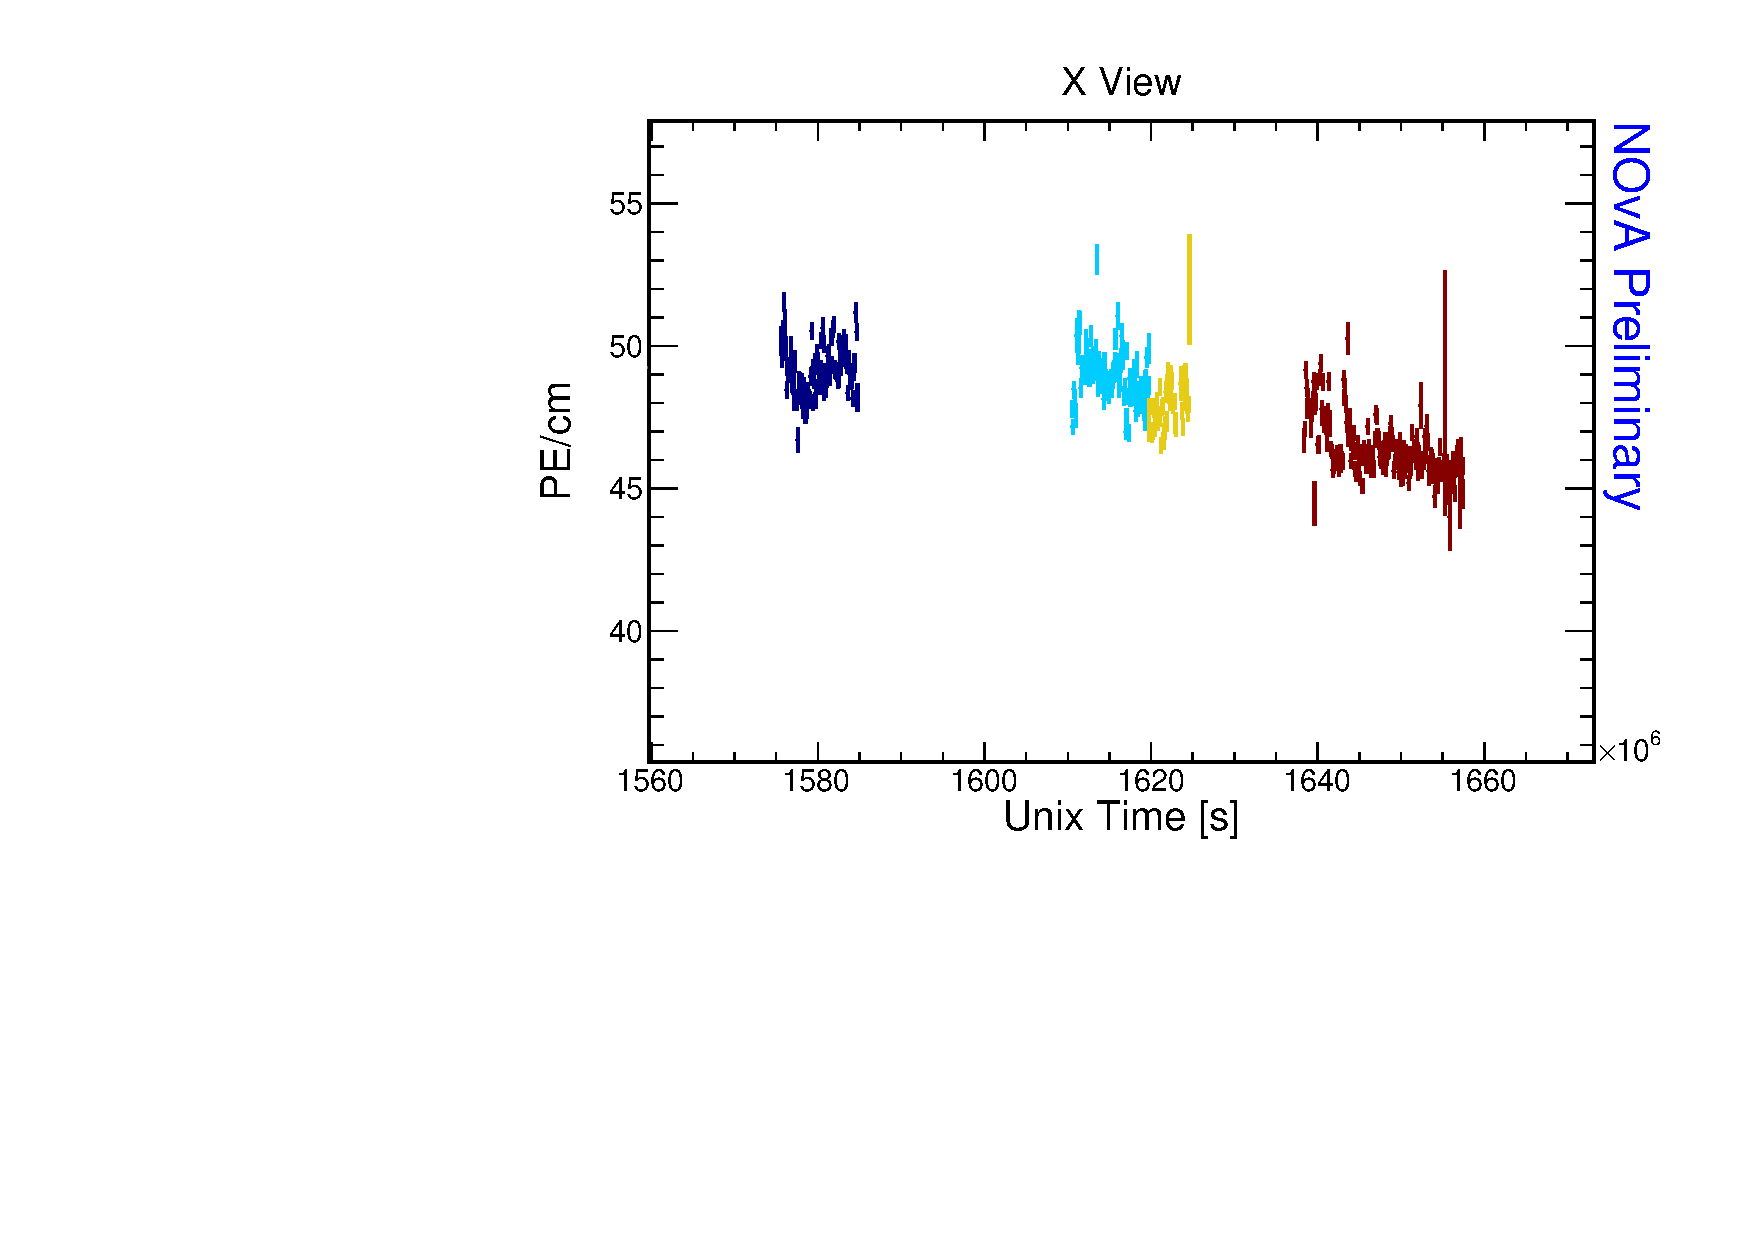
\includegraphics[width=\linewidth]{Plots/Calibana/pecm_time_x.pdf}
  \end{subfigure}
  \begin{subfigure}{0.495\textwidth}
    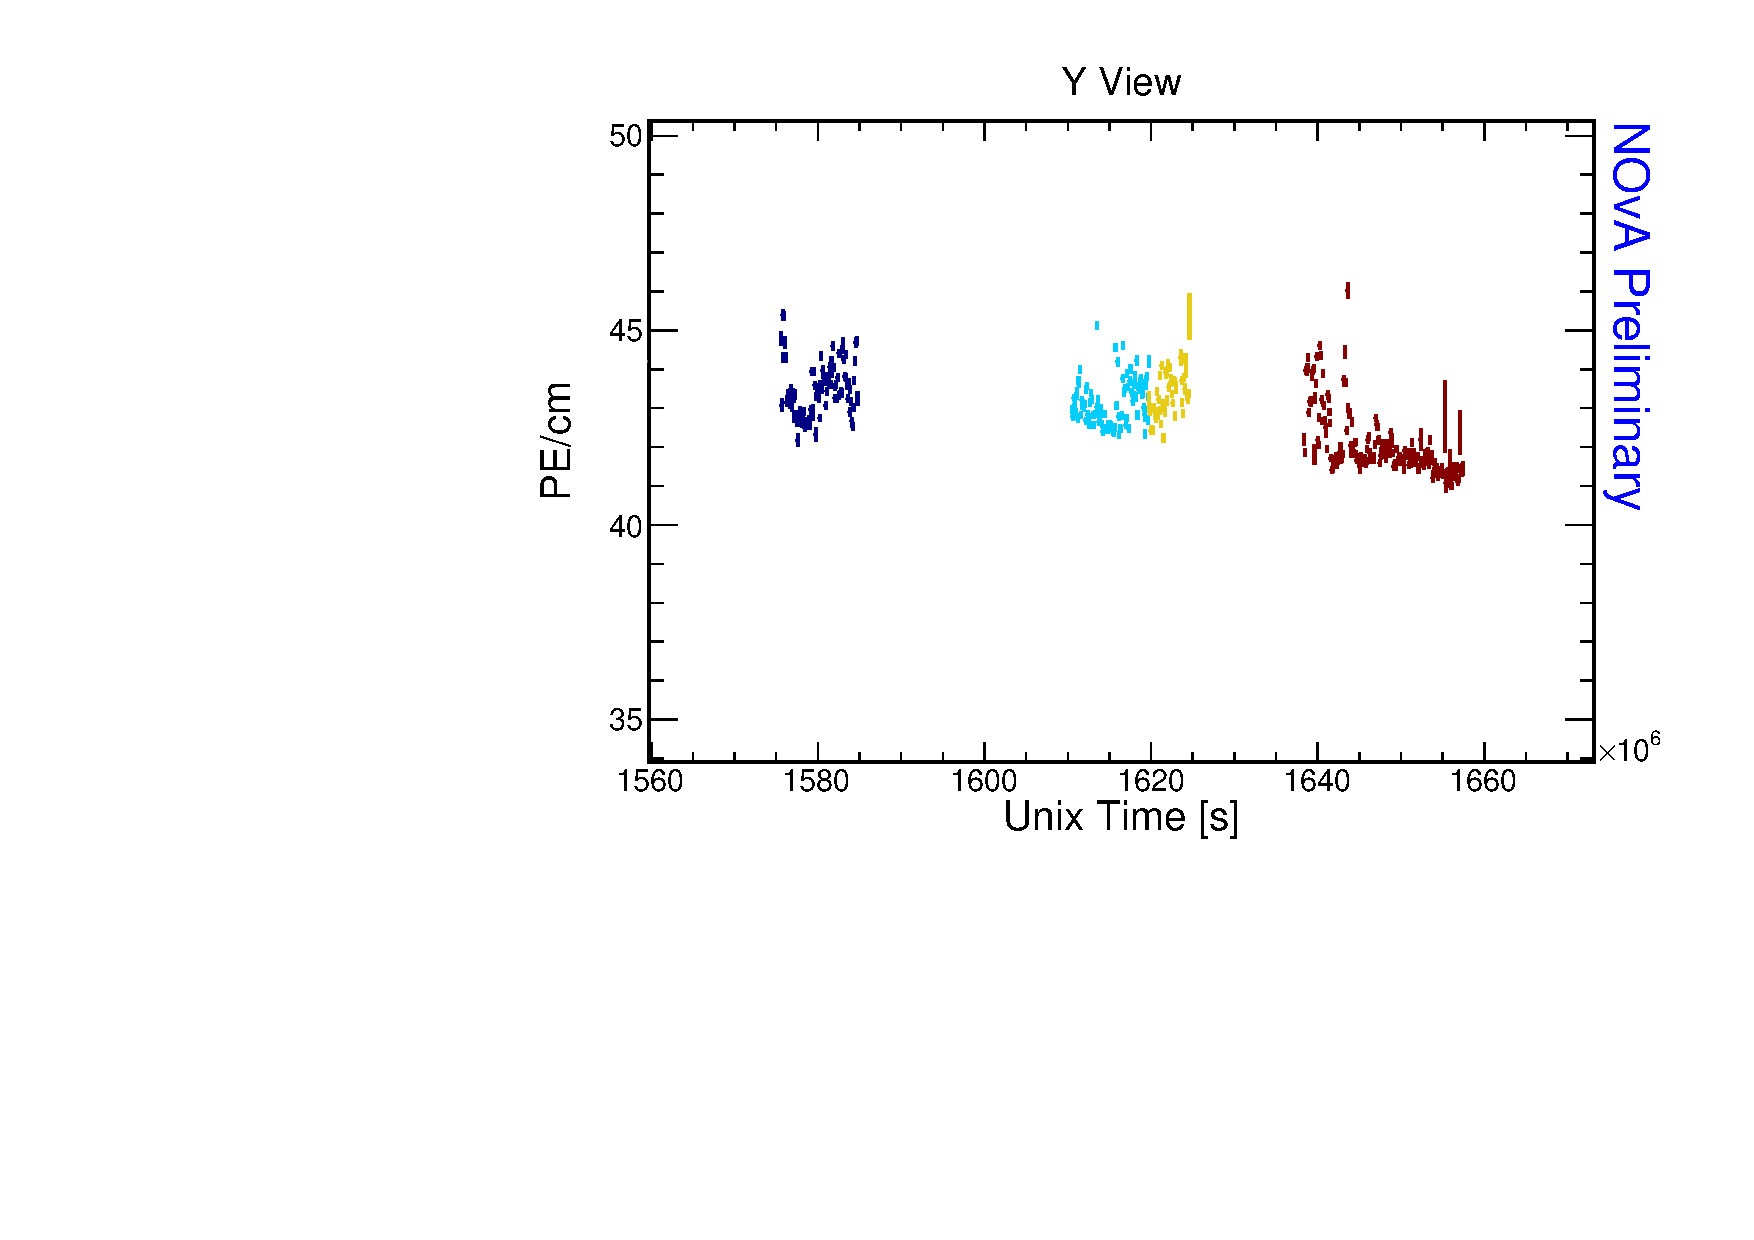
\includegraphics[width=\linewidth]{Plots/Calibana/pecm_time_y.pdf}
  \end{subfigure}
  \begin{subfigure}{0.495\textwidth}
    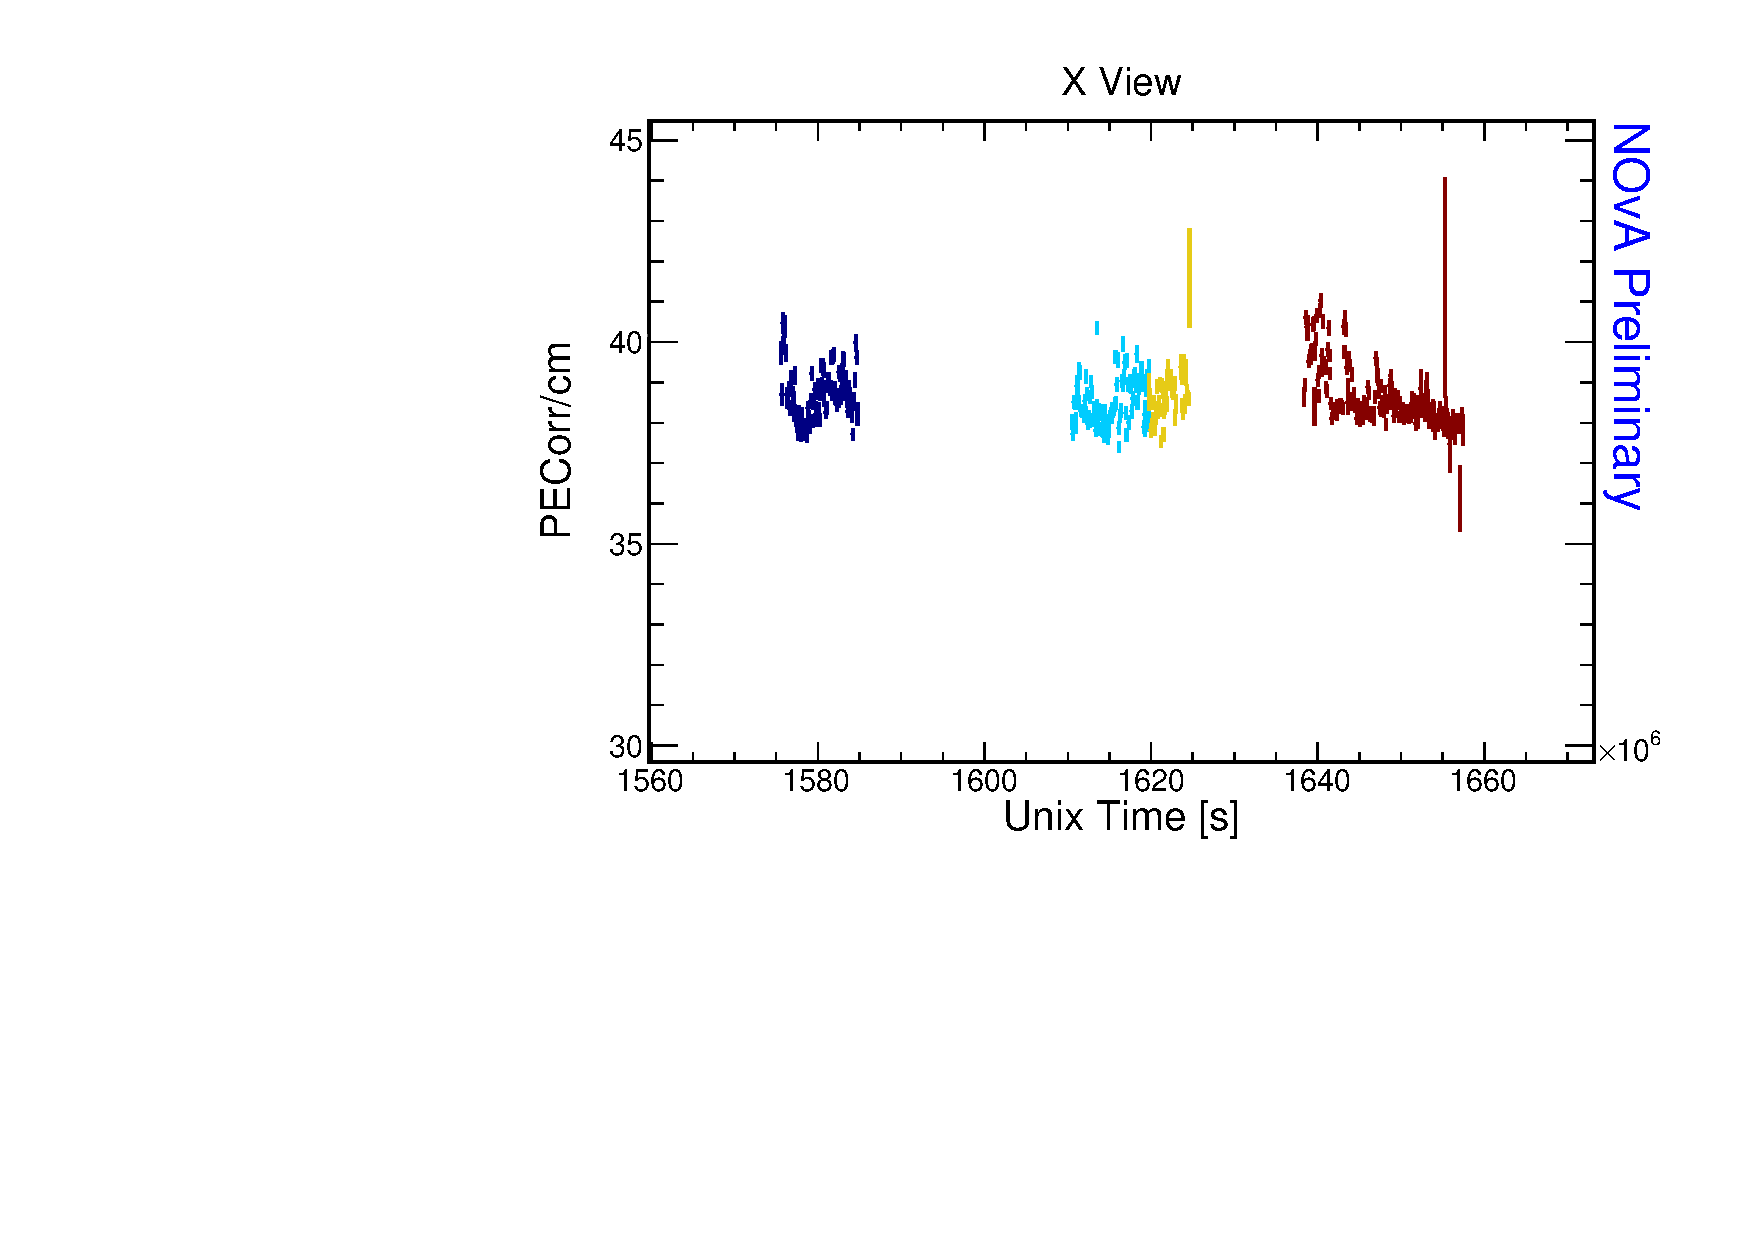
\includegraphics[width=\linewidth]{Plots/Calibana/pecorrcm_time_x.pdf}
  \end{subfigure}
  \begin{subfigure}{0.495\textwidth}
    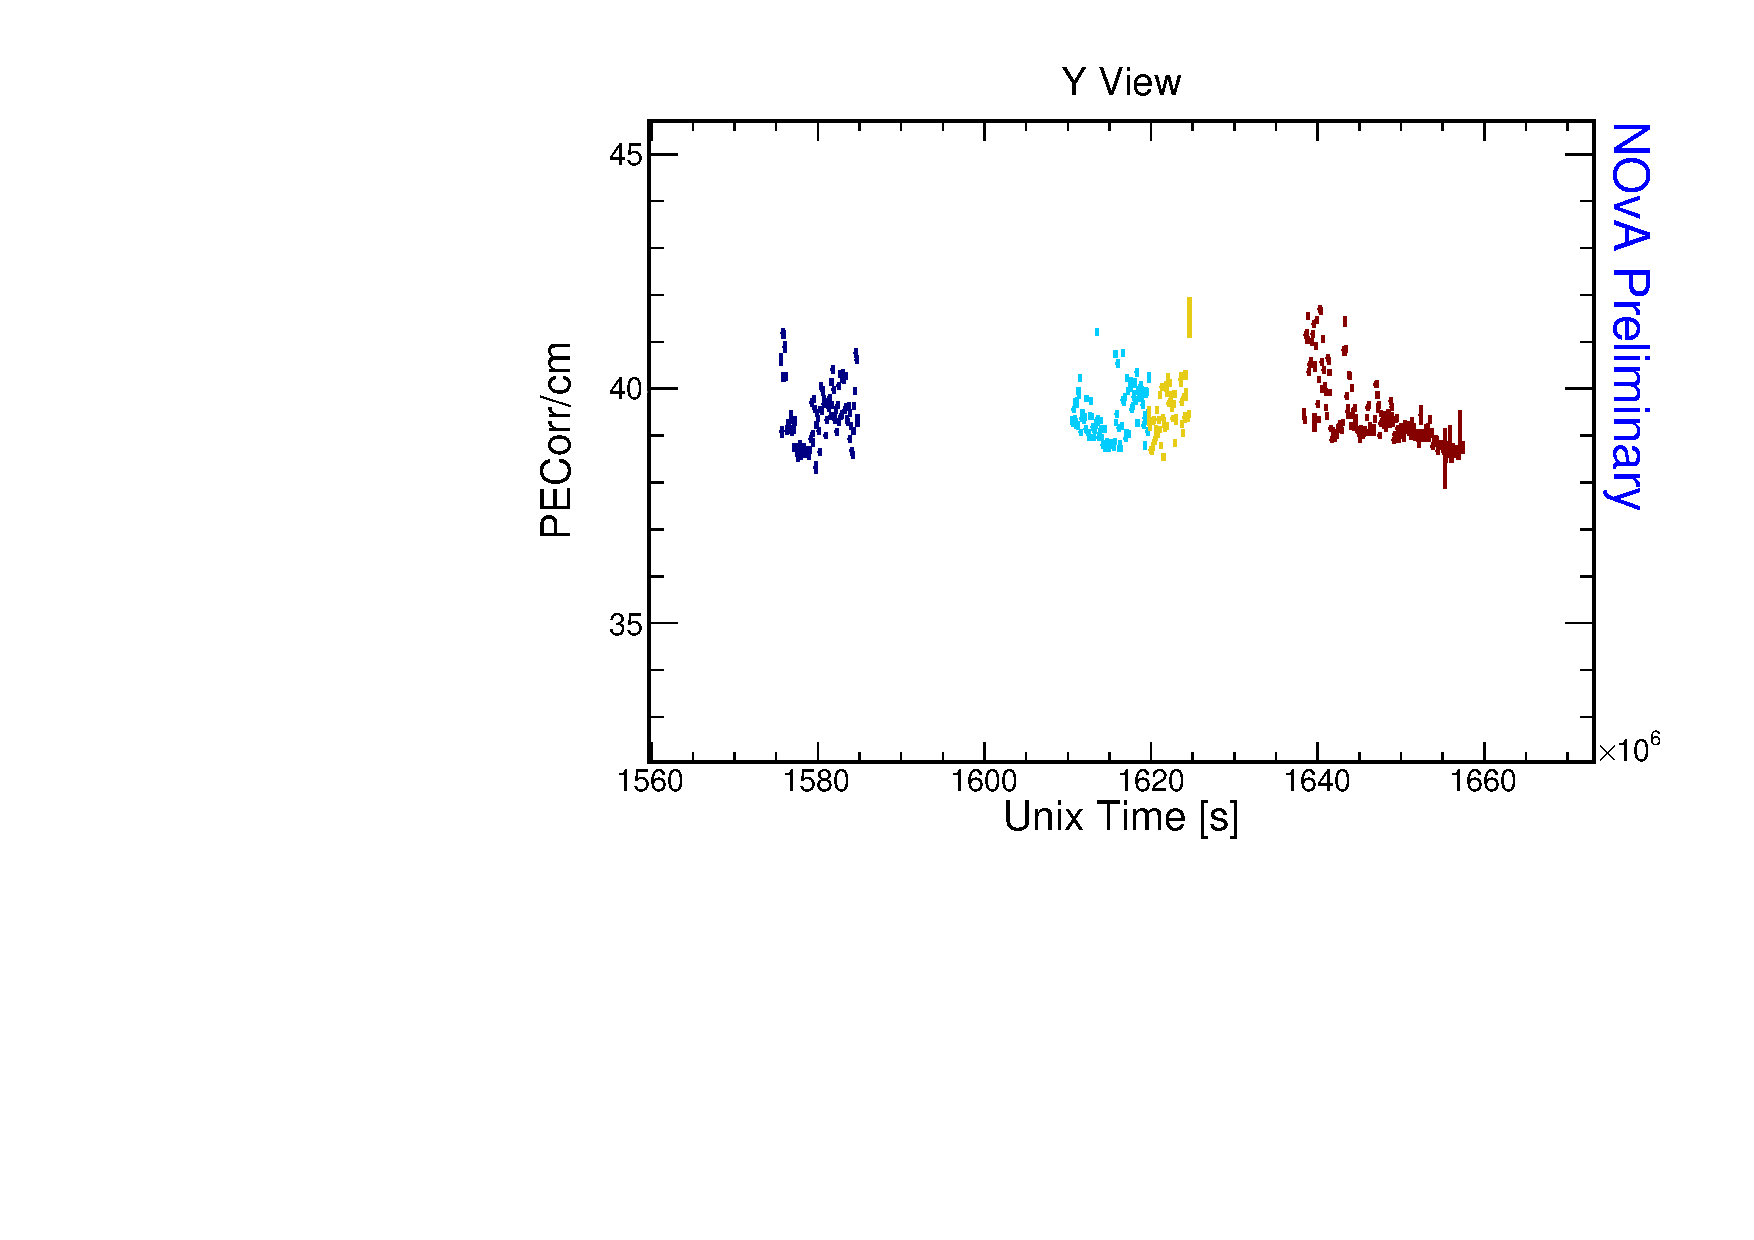
\includegraphics[width=\linewidth]{Plots/Calibana/pecorrcm_time_y.pdf}
  \end{subfigure}
    \begin{subfigure}{0.495\textwidth}
    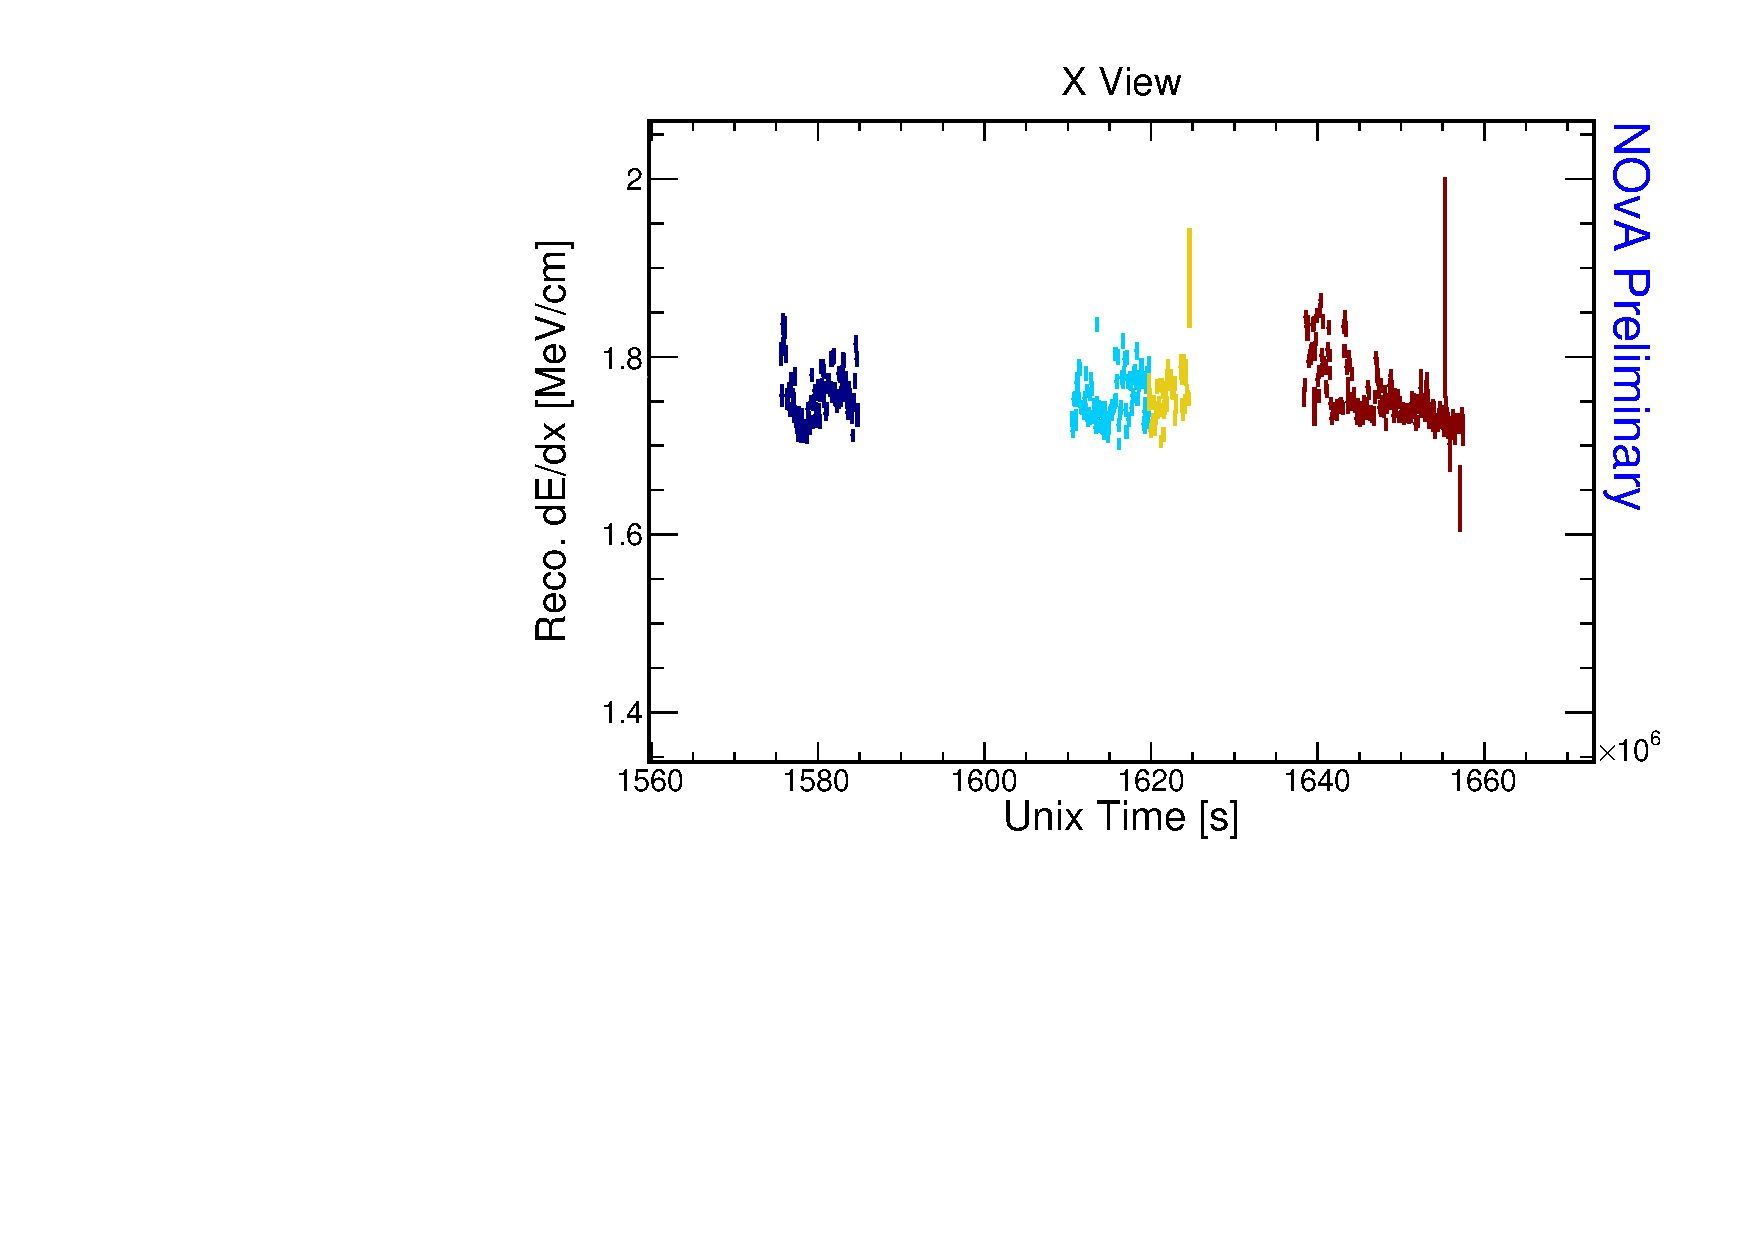
\includegraphics[width=\linewidth]{Plots/Calibana/recomevcm_time_x.pdf}
  \end{subfigure}
  \begin{subfigure}{0.495\textwidth}
    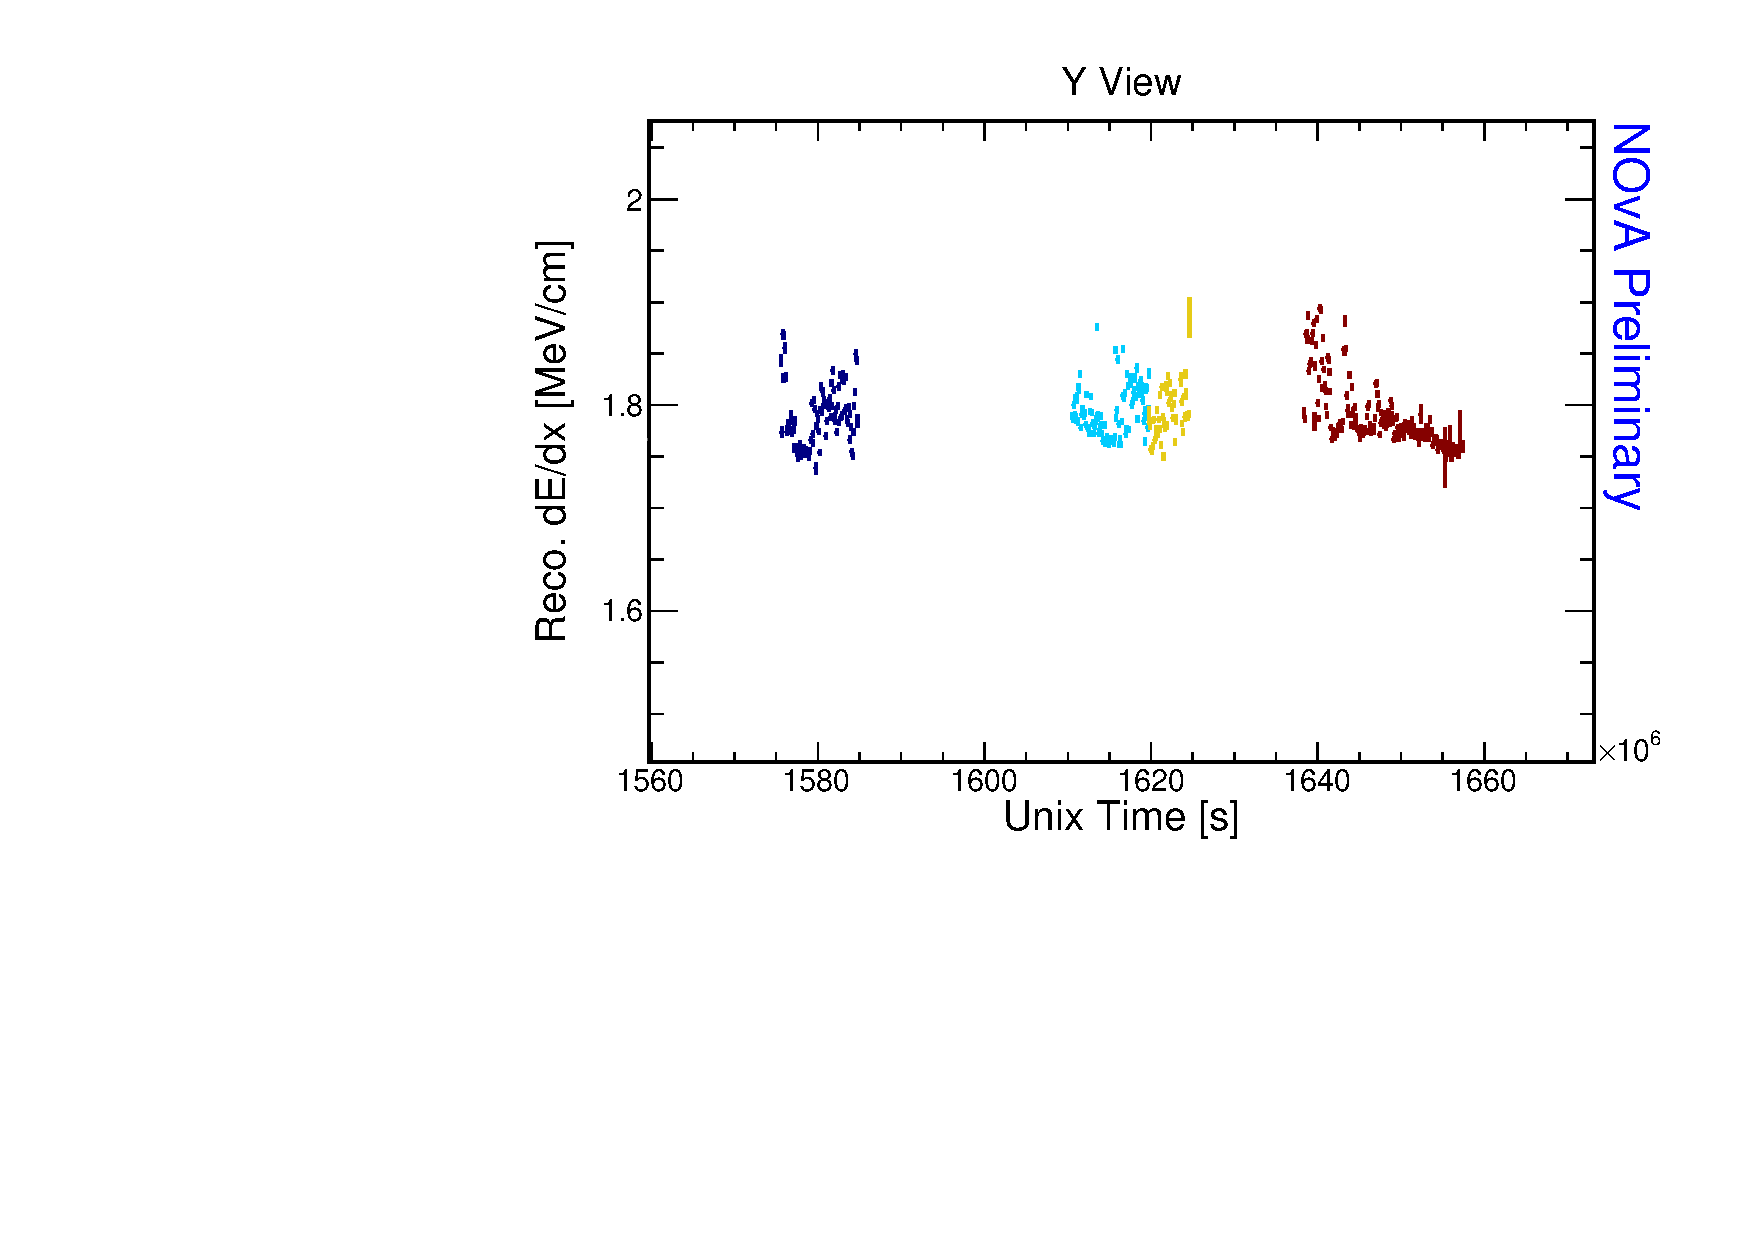
\includegraphics[width=\linewidth]{Plots/Calibana/recomevcm_time_y.pdf}
  \end{subfigure}
  \caption[Energy deposition of stopping muons as a function of time]{Distributions of stopping muons within a 1-2 m track window from the end of their tracks as a function of time for the Test Beam data samples. The top row shows the energy deposition before any correction, middle row after relative calibration corrections and bottom row after full calibration corrections. The left column shows the X view (vertical planes) and right column the Y view (horizontal planes).}
  %\label{fig:AbsCalibDrift1}
\end{figure}

\begin{figure}[!ht]
  \begin{subfigure}{\textwidth}
    \centering
    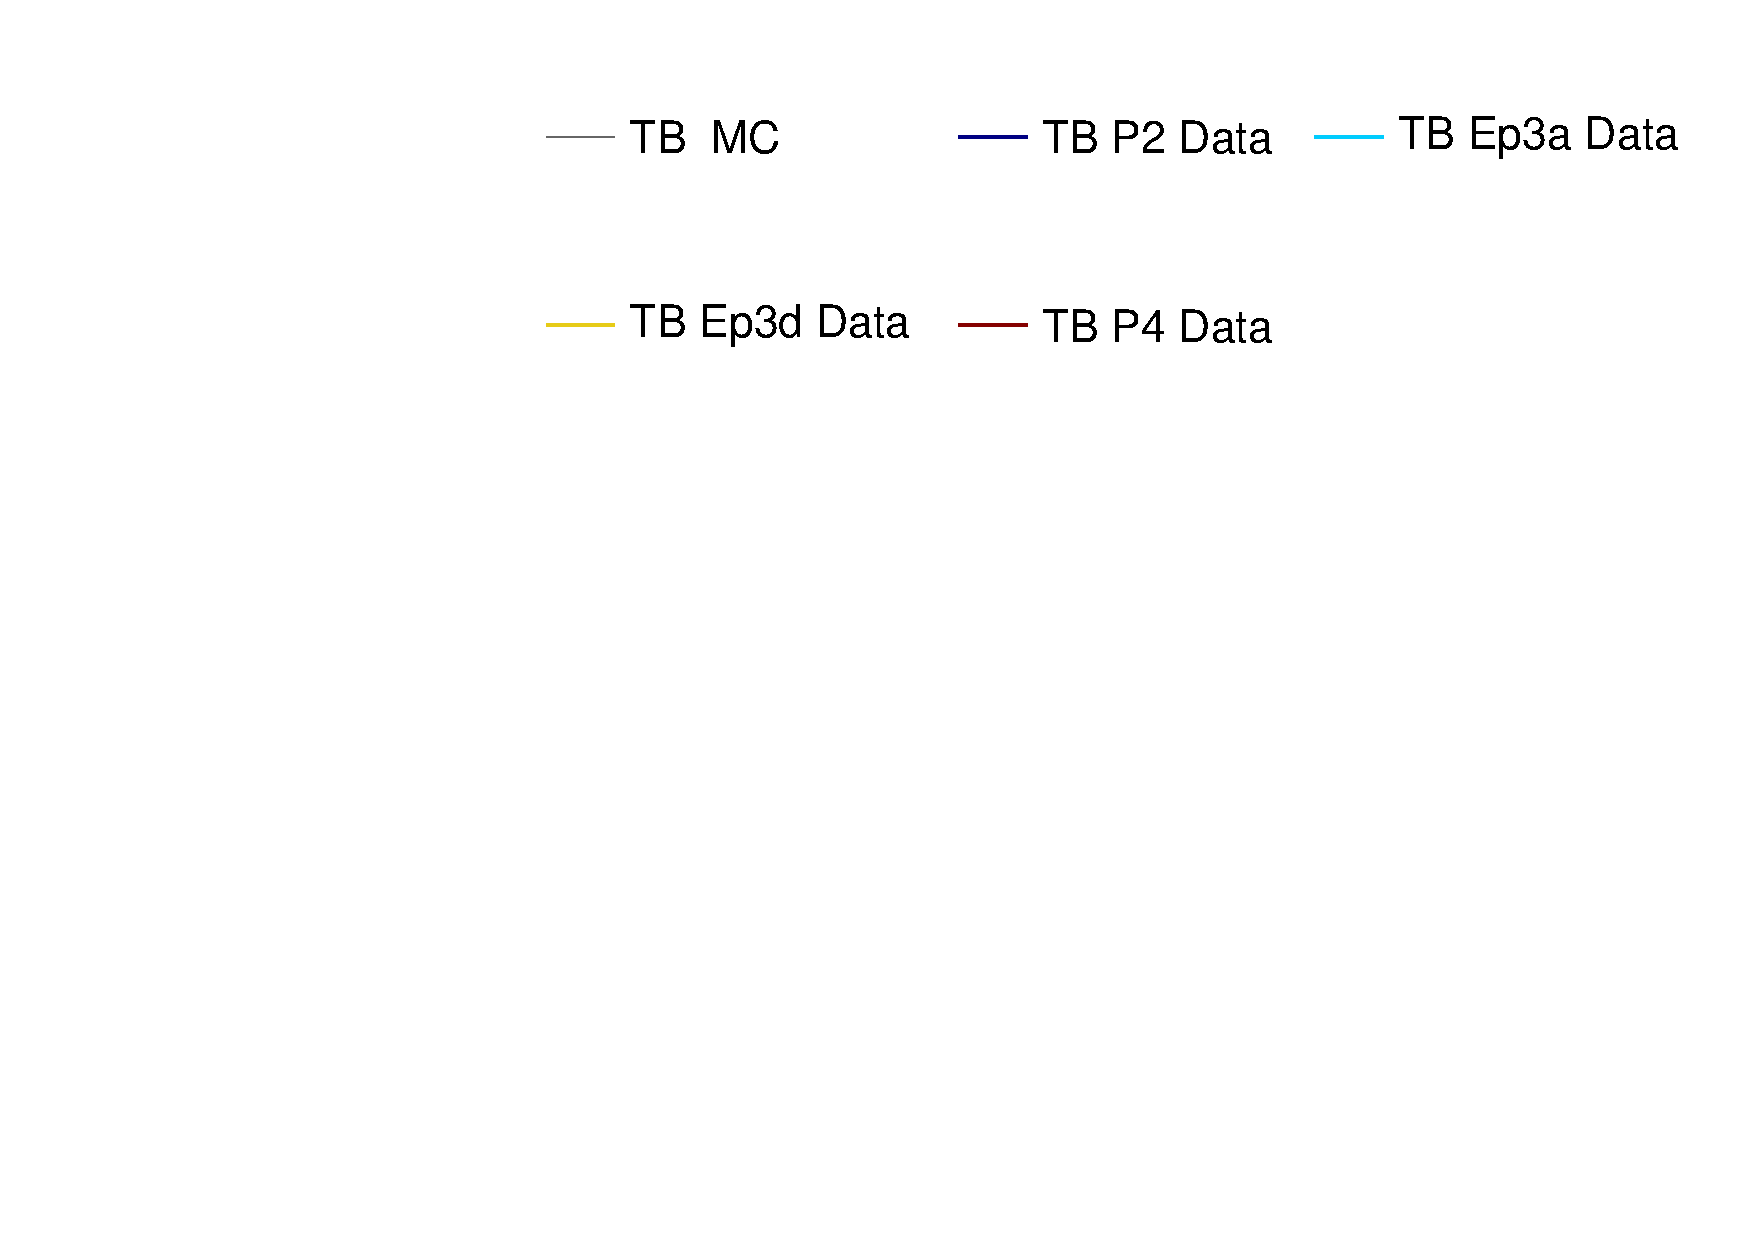
\includegraphics[height=0.2\linewidth]{Plots/Calibana/legend.pdf}
  \end{subfigure}
  \vspace*{2mm}
  
  \begin{subfigure}{0.495\textwidth}
    \includegraphics[width=\linewidth]{Plots/Calibana/pe_time_x.pdf}
  \end{subfigure}
  \begin{subfigure}{0.495\textwidth}
    \includegraphics[width=\linewidth]{Plots/Calibana/pe_time_y.pdf}
  \end{subfigure}
  \begin{subfigure}{0.495\textwidth}
    \includegraphics[width=\linewidth]{Plots/Calibana/pecorr_time_x.pdf}
  \end{subfigure}
  \begin{subfigure}{0.495\textwidth}
    \includegraphics[width=\linewidth]{Plots/Calibana/pecorr_time_y.pdf}
  \end{subfigure}
  \begin{subfigure}{0.495\textwidth}
    \includegraphics[width=\linewidth]{Plots/Calibana/cm_time_x.pdf}
  \end{subfigure}
  \begin{subfigure}{0.495\textwidth}
    \includegraphics[width=\linewidth]{Plots/Calibana/cm_time_y.pdf}
  \end{subfigure}
  \caption[Calibration variables of stopping muons as a function of time]{Distributions of stopping muons within a 1-2 m track window from the end of their tracks as a function of time for simulation (gray) and all the Test Beam data samples. The top row shows the number of recorded photo electrons before any corrections, middle row shows the same after relative calibration corrections and bottom row shows the path length through the cell. The left column shows the X view (vertical planes) and right column the Y view (horizontal planes).}
  %\label{fig:AbsCalibDrift2}
\end{figure}


\begin{figure}[ht!]
  \begin{subfigure}{\textwidth}
	\centering
   	\includegraphics[height=0.2\linewidth]{Plots/Calibana/legend.pdf}
  \end{subfigure}
  \vspace*{2mm}
  
  \begin{subfigure}{0.495\textwidth}
    \includegraphics[width=\linewidth]{Plots/Calibana/nhits_w_x.pdf}
  \end{subfigure}
  \begin{subfigure}{0.495\textwidth}
    \includegraphics[width=\linewidth]{Plots/Calibana/nhits_w_y.pdf}
  \end{subfigure}
  \begin{subfigure}{0.495\textwidth}
    \includegraphics[width=\linewidth]{Plots/Calibana/nhits_cell_x.pdf}
  \end{subfigure}
  \begin{subfigure}{0.495\textwidth}
    \includegraphics[width=\linewidth]{Plots/Calibana/nhits_cell_y.pdf}
  \end{subfigure}
  \begin{subfigure}{0.495\textwidth}
    \includegraphics[width=\linewidth]{Plots/Calibana/nhits_plane_x.pdf}
  \end{subfigure}
  \begin{subfigure}{0.495\textwidth}
    \includegraphics[width=\linewidth]{Plots/Calibana/nhits_plane_y.pdf}
  \end{subfigure}
    \caption[Distribution of calibration variables of stopping muons]{Distributions of the variables used in the calibration of stopping muons within a 1-2 m track window from the end of their tracks for simulation (gray) and all the Test Beam data samples. The top row shows the position within a cell, middle row the cell number and bottom row the plane number. The left column shows the X view (vertical planes) and right column the Y view (horizontal planes).}
  %\label{fig:AbsCalibNHitsWCellPlane}
\end{figure}

\FloatBarrier
\section{Distributions for through-going muons}

\begin{figure}[!ht]
  \begin{subfigure}{0.495\textwidth}
    \includegraphics[width=\linewidth]{Plots/PCListAna/DataAndSim_pecm_ts_w_X.pdf}
  \end{subfigure}
  \begin{subfigure}{0.495\textwidth}
    \includegraphics[width=\linewidth]{Plots/PCListAna/DataAndSim_pecm_ts_w_y.pdf}
  \end{subfigure}
  \begin{subfigure}{0.495\textwidth}
    \includegraphics[width=\linewidth]{Plots/PCListAna/DataAndSim_pecorrcm_ts_w_x.pdf}
  \end{subfigure}
  \begin{subfigure}{0.495\textwidth}
    \includegraphics[width=\linewidth]{Plots/PCListAna/DataAndSim_pecorrcm_ts_w_y.pdf}
  \end{subfigure}
    \begin{subfigure}{0.495\textwidth}
    \includegraphics[width=\linewidth]{Plots/PCListAna/DataAndSim_recomevcm_ts_w_x.pdf}
  \end{subfigure}
  \begin{subfigure}{0.495\textwidth}
    \includegraphics[width=\linewidth]{Plots/PCListAna/DataAndSim_recomevcm_ts_w_y.pdf}
  \end{subfigure}
  \caption[Validation plots for through-going muons along w]{Distributions of through-going cosmic muons with $w\in\left(-80,80\right)\unit{cm}$ as a function of $w$ for stable runs in the Test Beam period 4 data (black) and data-based simulation (red). Bottom panel of each plot shows the ratio of each bin and the mean y axis, separately for data and simulation. Discrepancy in the right-most bin is solely due to binning.}
\end{figure}

\begin{figure}[!ht]
  \begin{subfigure}{0.495\textwidth}
    \includegraphics[width=\linewidth]{Plots/PCListAna/DataAndSim_pe_w_x.pdf}
  \end{subfigure}
  \begin{subfigure}{0.495\textwidth}
    \includegraphics[width=\linewidth]{Plots/PCListAna/DataAndSim_pe_w_y.pdf}
  \end{subfigure}
  \begin{subfigure}{0.495\textwidth}
    \includegraphics[width=\linewidth]{Plots/PCListAna/DataAndSim_pecorr_w_x.pdf}
  \end{subfigure}
  \begin{subfigure}{0.495\textwidth}
    \includegraphics[width=\linewidth]{Plots/PCListAna/DataAndSim_pecorr_w_y.pdf}
  \end{subfigure}
  \begin{subfigure}{0.495\textwidth}
    \includegraphics[width=\linewidth]{Plots/PCListAna/DataAndSim_cm_w_x.pdf}
  \end{subfigure}
  \begin{subfigure}{0.495\textwidth}
    \includegraphics[width=\linewidth]{Plots/PCListAna/DataAndSim_cm_w_y.pdf}
  \end{subfigure}
  \caption[Validation plots for through-going muons along w]{Distributions of through-going cosmic muons with $w\in\left(-80,80\right)\unit{cm}$ as a function of $w$ for stable runs in the Test Beam period 4 data (black) and data-based simulation (red). Bottom panel of each plot shows the ratio of each bin and the mean y axis, separately for data and simulation. Discrepancy in the right-most bin is solely due to binning.}
\end{figure}

\begin{figure}[!ht]
  \begin{subfigure}{0.495\textwidth}
    \includegraphics[width=\linewidth]{Plots/PCListAna/DataAndSim_pecm_ts_cell_X.pdf}
  \end{subfigure}
  \begin{subfigure}{0.495\textwidth}
    \includegraphics[width=\linewidth]{Plots/PCListAna/DataAndSim_pecm_ts_cell_y.pdf}
  \end{subfigure}
  \begin{subfigure}{0.495\textwidth}
    \includegraphics[width=\linewidth]{Plots/PCListAna/DataAndSim_pecorrcm_ts_cell_x.pdf}
  \end{subfigure}
  \begin{subfigure}{0.495\textwidth}
    \includegraphics[width=\linewidth]{Plots/PCListAna/DataAndSim_pecorrcm_ts_cell_y.pdf}
  \end{subfigure}
    \begin{subfigure}{0.495\textwidth}
    \includegraphics[width=\linewidth]{Plots/PCListAna/DataAndSim_recomevcm_ts_cell_x.pdf}
  \end{subfigure}
  \begin{subfigure}{0.495\textwidth}
    \includegraphics[width=\linewidth]{Plots/PCListAna/DataAndSim_recomevcm_ts_cell_y.pdf}
  \end{subfigure}
  \caption[Validation plots for through-going muons across cells]{Distributions of through-going cosmic muons with $w\in\left(-80,80\right)\unit{cm}$ as a function of cell number for stable runs in the Test Beam period 4 data (black) and data-based simulation (red). Bottom panel of each plot shows the ratio of each bin and the mean y axis, separately for data and simulation.}
\end{figure}

\begin{figure}[!ht]
  \begin{subfigure}{0.495\textwidth}
    \includegraphics[width=\linewidth]{Plots/PCListAna/DataAndSim_pe_cell_x.pdf}
  \end{subfigure}
  \begin{subfigure}{0.495\textwidth}
    \includegraphics[width=\linewidth]{Plots/PCListAna/DataAndSim_pe_cell_y.pdf}
  \end{subfigure}
  \begin{subfigure}{0.495\textwidth}
    \includegraphics[width=\linewidth]{Plots/PCListAna/DataAndSim_pecorr_cell_x.pdf}
  \end{subfigure}
  \begin{subfigure}{0.495\textwidth}
    \includegraphics[width=\linewidth]{Plots/PCListAna/DataAndSim_pecorr_cell_y.pdf}
  \end{subfigure}
  \begin{subfigure}{0.495\textwidth}
    \includegraphics[width=\linewidth]{Plots/PCListAna/DataAndSim_cm_cell_x.pdf}
  \end{subfigure}
  \begin{subfigure}{0.495\textwidth}
    \includegraphics[width=\linewidth]{Plots/PCListAna/DataAndSim_cm_cell_y.pdf}
  \end{subfigure}
  \caption[Validation plots for through-going muons across cells]{Distributions of through-going cosmic muons with $w\in\left(-80,80\right)\unit{cm}$ as a function of cell number for stable runs in the Test Beam period 4 data (black) and data-based simulation (red). Bottom panel of each plot shows the ratio of each bin and the mean y axis, separately for data and simulation.}
\end{figure}

\begin{figure}[!ht]
  \begin{subfigure}{0.495\textwidth}
    \includegraphics[width=\linewidth]{Plots/PCListAna/DataAndSim_pecm_ts_plane_X.pdf}
  \end{subfigure}
  \begin{subfigure}{0.495\textwidth}
    \includegraphics[width=\linewidth]{Plots/PCListAna/DataAndSim_pecm_ts_plane_y.pdf}
  \end{subfigure}
  \begin{subfigure}{0.495\textwidth}
    \includegraphics[width=\linewidth]{Plots/PCListAna/DataAndSim_pecorrcm_ts_plane_x.pdf}
  \end{subfigure}
  \begin{subfigure}{0.495\textwidth}
    \includegraphics[width=\linewidth]{Plots/PCListAna/DataAndSim_pecorrcm_ts_plane_y.pdf}
  \end{subfigure}
    \begin{subfigure}{0.495\textwidth}
    \includegraphics[width=\linewidth]{Plots/PCListAna/DataAndSim_recomevcm_ts_plane_x.pdf}
  \end{subfigure}
  \begin{subfigure}{0.495\textwidth}
    \includegraphics[width=\linewidth]{Plots/PCListAna/DataAndSim_recomevcm_ts_plane_y.pdf}
  \end{subfigure}
  \caption[Validation plots for through-going muons across planes]{Distributions of through-going cosmic muons with $w\in\left(-80,80\right)\unit{cm}$ as a function of plane number for stable runs in the Test Beam period 4 data (black) and data-based simulation (red). Bottom panel of each plot shows the ratio of each bin and the mean y axis, separately for data and simulation.}
\end{figure}

\begin{figure}[!ht]
  \begin{subfigure}{0.495\textwidth}
    \includegraphics[width=\linewidth]{Plots/PCListAna/DataAndSim_pe_plane_x.pdf}
  \end{subfigure}
  \begin{subfigure}{0.495\textwidth}
    \includegraphics[width=\linewidth]{Plots/PCListAna/DataAndSim_pe_plane_y.pdf}
  \end{subfigure}
  \begin{subfigure}{0.495\textwidth}
    \includegraphics[width=\linewidth]{Plots/PCListAna/DataAndSim_pecorr_plane_x.pdf}
  \end{subfigure}
  \begin{subfigure}{0.495\textwidth}
    \includegraphics[width=\linewidth]{Plots/PCListAna/DataAndSim_pecorr_plane_y.pdf}
  \end{subfigure}
  \begin{subfigure}{0.495\textwidth}
    \includegraphics[width=\linewidth]{Plots/PCListAna/DataAndSim_cm_plane_x.pdf}
  \end{subfigure}
  \begin{subfigure}{0.495\textwidth}
    \includegraphics[width=\linewidth]{Plots/PCListAna/DataAndSim_cm_plane_y.pdf}
  \end{subfigure}
  \caption[Validation plots for through-going muons across planes]{Distributions of through-going cosmic muons with $w\in\left(-80,80\right)\unit{cm}$ as a function of plane number for stable runs in the Test Beam period 4 data (black) and data-based simulation (red). Bottom panel of each plot shows the ratio of each bin and the mean y axis, separately for data and simulation.}
\end{figure}

\begin{figure}[!ht]
  \begin{subfigure}{0.495\textwidth}
    \includegraphics[width=\linewidth]{Plots/PCListAna/DataAndSim_pecm_ts_cosx_X.pdf}
  \end{subfigure}
  \begin{subfigure}{0.495\textwidth}
    \includegraphics[width=\linewidth]{Plots/PCListAna/DataAndSim_pecm_ts_cosx_y.pdf}
  \end{subfigure}
  \begin{subfigure}{0.495\textwidth}
    \includegraphics[width=\linewidth]{Plots/PCListAna/DataAndSim_pecorrcm_ts_cosx_x.pdf}
  \end{subfigure}
  \begin{subfigure}{0.495\textwidth}
    \includegraphics[width=\linewidth]{Plots/PCListAna/DataAndSim_pecorrcm_ts_cosx_y.pdf}
  \end{subfigure}
    \begin{subfigure}{0.495\textwidth}
    \includegraphics[width=\linewidth]{Plots/PCListAna/DataAndSim_recomevcm_ts_cosx_x.pdf}
  \end{subfigure}
  \begin{subfigure}{0.495\textwidth}
    \includegraphics[width=\linewidth]{Plots/PCListAna/DataAndSim_recomevcm_ts_cosx_y.pdf}
  \end{subfigure}
  \caption[Validation plots for through-going muons along angle from the x axis]{Distributions of through-going cosmic muons with $w\in\left(-80,80\right)\unit{cm}$ as a function of the cosine of the angle from the x axis for stable runs in the Test Beam period 4 data (black) and data-based simulation (red). Bottom panel of each plot shows the ratio of each bin and the mean y axis, separately for data and simulation.}
\end{figure}

\begin{figure}[!ht]
  \begin{subfigure}{0.495\textwidth}
    \includegraphics[width=\linewidth]{Plots/PCListAna/DataAndSim_pe_cosx_x.pdf}
  \end{subfigure}
  \begin{subfigure}{0.495\textwidth}
    \includegraphics[width=\linewidth]{Plots/PCListAna/DataAndSim_pe_cosx_y.pdf}
  \end{subfigure}
  \begin{subfigure}{0.495\textwidth}
    \includegraphics[width=\linewidth]{Plots/PCListAna/DataAndSim_pecorr_cosx_x.pdf}
  \end{subfigure}
  \begin{subfigure}{0.495\textwidth}
    \includegraphics[width=\linewidth]{Plots/PCListAna/DataAndSim_pecorr_cosx_y.pdf}
  \end{subfigure}
  \begin{subfigure}{0.495\textwidth}
    \includegraphics[width=\linewidth]{Plots/PCListAna/DataAndSim_cm_cosx_x.pdf}
  \end{subfigure}
  \begin{subfigure}{0.495\textwidth}
    \includegraphics[width=\linewidth]{Plots/PCListAna/DataAndSim_cm_cosx_y.pdf}
  \end{subfigure}
  \caption[Validation plots for through-going muons along angle from the x axis]{Distributions of through-going cosmic muons with $w\in\left(-80,80\right)\unit{cm}$ as a function of the cosine of the angle from the x axis for stable runs in the Test Beam period 4 data (black) and data-based simulation (red). Bottom panel of each plot shows the ratio of each bin and the mean y axis, separately for data and simulation.}
\end{figure}

\begin{figure}[!ht]
  \begin{subfigure}{0.495\textwidth}
    \includegraphics[width=\linewidth]{Plots/PCListAna/DataAndSim_pecm_ts_cosy_X.pdf}
  \end{subfigure}
  \begin{subfigure}{0.495\textwidth}
    \includegraphics[width=\linewidth]{Plots/PCListAna/DataAndSim_pecm_ts_cosy_y.pdf}
  \end{subfigure}
  \begin{subfigure}{0.495\textwidth}
    \includegraphics[width=\linewidth]{Plots/PCListAna/DataAndSim_pecorrcm_ts_cosy_x.pdf}
  \end{subfigure}
  \begin{subfigure}{0.495\textwidth}
    \includegraphics[width=\linewidth]{Plots/PCListAna/DataAndSim_pecorrcm_ts_cosy_y.pdf}
  \end{subfigure}
    \begin{subfigure}{0.495\textwidth}
    \includegraphics[width=\linewidth]{Plots/PCListAna/DataAndSim_recomevcm_ts_cosy_x.pdf}
  \end{subfigure}
  \begin{subfigure}{0.495\textwidth}
    \includegraphics[width=\linewidth]{Plots/PCListAna/DataAndSim_recomevcm_ts_cosy_y.pdf}
  \end{subfigure}
  \caption[Validation plots for through-going muons along angle from the y axis]{Distributions of through-going cosmic muons with $w\in\left(-80,80\right)\unit{cm}$ as a function of the cosine of the angle from the y axis for stable runs in the Test Beam period 4 data (black) and data-based simulation (red). Bottom panel of each plot shows the ratio of each bin and the mean y axis, separately for data and simulation.}
\end{figure}

\begin{figure}[!ht]
  \begin{subfigure}{0.495\textwidth}
    \includegraphics[width=\linewidth]{Plots/PCListAna/DataAndSim_pe_cosy_x.pdf}
  \end{subfigure}
  \begin{subfigure}{0.495\textwidth}
    \includegraphics[width=\linewidth]{Plots/PCListAna/DataAndSim_pe_cosy_y.pdf}
  \end{subfigure}
  \begin{subfigure}{0.495\textwidth}
    \includegraphics[width=\linewidth]{Plots/PCListAna/DataAndSim_pecorr_cosy_x.pdf}
  \end{subfigure}
  \begin{subfigure}{0.495\textwidth}
    \includegraphics[width=\linewidth]{Plots/PCListAna/DataAndSim_pecorr_cosy_y.pdf}
  \end{subfigure}
  \begin{subfigure}{0.495\textwidth}
    \includegraphics[width=\linewidth]{Plots/PCListAna/DataAndSim_cm_cosy_x.pdf}
  \end{subfigure}
  \begin{subfigure}{0.495\textwidth}
    \includegraphics[width=\linewidth]{Plots/PCListAna/DataAndSim_cm_cosy_y.pdf}
  \end{subfigure}
  \caption[Validation plots for through-going muons along angle from the y axis]{Distributions of through-going cosmic muons with $w\in\left(-80,80\right)\unit{cm}$ as a function of the cosine of the angle from the y axis for stable runs in the Test Beam period 4 data (black) and data-based simulation (red). Bottom panel of each plot shows the ratio of each bin and the mean y axis, separately for data and simulation.}
\end{figure}

\begin{figure}[!ht]
  \begin{subfigure}{0.495\textwidth}
    \includegraphics[width=\linewidth]{Plots/PCListAna/DataAndSim_pecm_ts_cosz_X.pdf}
  \end{subfigure}
  \begin{subfigure}{0.495\textwidth}
    \includegraphics[width=\linewidth]{Plots/PCListAna/DataAndSim_pecm_ts_cosz_y.pdf}
  \end{subfigure}
  \begin{subfigure}{0.495\textwidth}
    \includegraphics[width=\linewidth]{Plots/PCListAna/DataAndSim_pecorrcm_ts_cosz_x.pdf}
  \end{subfigure}
  \begin{subfigure}{0.495\textwidth}
    \includegraphics[width=\linewidth]{Plots/PCListAna/DataAndSim_pecorrcm_ts_cosz_y.pdf}
  \end{subfigure}
    \begin{subfigure}{0.495\textwidth}
    \includegraphics[width=\linewidth]{Plots/PCListAna/DataAndSim_recomevcm_ts_cosz_x.pdf}
  \end{subfigure}
  \begin{subfigure}{0.495\textwidth}
    \includegraphics[width=\linewidth]{Plots/PCListAna/DataAndSim_recomevcm_ts_cosz_y.pdf}
  \end{subfigure}
  \caption[Validation plots for through-going muons along angle from the z axis]{Distributions of through-going cosmic muons with $w\in\left(-80,80\right)\unit{cm}$ as a function of the cosine of the angle from the z axis for stable runs in the Test Beam period 4 data (black) and data-based simulation (red). Bottom panel of each plot shows the ratio of each bin and the mean y axis, separately for data and simulation.}
\end{figure}

\begin{figure}[!ht]
  \begin{subfigure}{0.495\textwidth}
    \includegraphics[width=\linewidth]{Plots/PCListAna/DataAndSim_pe_cosz_x.pdf}
  \end{subfigure}
  \begin{subfigure}{0.495\textwidth}
    \includegraphics[width=\linewidth]{Plots/PCListAna/DataAndSim_pe_cosz_y.pdf}
  \end{subfigure}
  \begin{subfigure}{0.495\textwidth}
    \includegraphics[width=\linewidth]{Plots/PCListAna/DataAndSim_pecorr_cosz_x.pdf}
  \end{subfigure}
  \begin{subfigure}{0.495\textwidth}
    \includegraphics[width=\linewidth]{Plots/PCListAna/DataAndSim_pecorr_cosz_y.pdf}
  \end{subfigure}
  \begin{subfigure}{0.495\textwidth}
    \includegraphics[width=\linewidth]{Plots/PCListAna/DataAndSim_cm_cosz_x.pdf}
  \end{subfigure}
  \begin{subfigure}{0.495\textwidth}
    \includegraphics[width=\linewidth]{Plots/PCListAna/DataAndSim_cm_cosz_y.pdf}
  \end{subfigure}
  \caption[Validation plots for through-going muons along angle from the z axis]{Distributions of through-going cosmic muons with $w\in\left(-80,80\right)\unit{cm}$ as a function of the cosine of the angle from the x axis for stable runs in the Test Beam period 4 data (black) and data-based simulation (red). Bottom panel of each plot shows the ratio of each bin and the mean y axis, separately for data and simulation.}
\end{figure}